%----------------------------------------------------------
% Folium: B.Tech project report (blackbook)
% Compile:  pdflatex report.tex  (run twice for contents and cross-references)
%----------------------------------------------------------
\documentclass[12pt]{report}
\usepackage[utf8]{inputenc}
\usepackage{graphicx}
\usepackage{longtable}
\usepackage{subcaption}
\usepackage[a4paper,width=150mm,top=25mm,bottom=25mm]{geometry}
\usepackage{amsmath,amssymb}
\usepackage{array,tabularx,multirow,makecell}
\usepackage{float}
\usepackage[table]{xcolor}
\usepackage{listings}
\usepackage{tikz}
\usepackage{enumitem}
\usepackage{parskip}
\usepackage{caption}
\usepackage[hidelinks]{hyperref}
\usepackage{url}

% Shared TikZ styles for every design diagram in the report.
\usetikzlibrary{positioning, arrows.meta, shapes.geometric, shapes.multipart, fit, calc, backgrounds}

\definecolor{tealfill}{RGB}{227,241,239}
\definecolor{tealline}{RGB}{42,127,122}
\definecolor{bluefill}{RGB}{233,239,249}
\definecolor{blueline}{RGB}{78,107,160}
\definecolor{greyfill}{RGB}{243,243,243}
\definecolor{greyline}{RGB}{120,120,120}
\definecolor{sandfill}{RGB}{252,244,228}
\definecolor{sandline}{RGB}{176,135,50}

\tikzset{
  >={Stealth[length=2.2mm]},
  every node/.style={font=\small, execute at begin node={\hyphenpenalty=10000\exhyphenpenalty=10000}},
  box/.style={draw=tealline, fill=tealfill, rounded corners=2pt, align=center,
              inner sep=4pt, minimum height=8mm, line width=0.6pt},
  mlbox/.style={box, draw=blueline, fill=bluefill},
  store/.style={box, draw=greyline, fill=greyfill},
  ext/.style={box, draw=sandline, fill=sandfill},
  tier/.style={draw=greyline, dashed, rounded corners=4pt, inner sep=6pt},
  tierlabel/.style={font=\footnotesize\itshape, text=greyline},
  flow/.style={->, line width=0.6pt},
  biflow/.style={<->, line width=0.6pt},
  lbl/.style={font=\footnotesize, fill=white, inner sep=1.5pt},
  proc/.style={circle, draw=tealline, fill=tealfill, align=center, minimum size=19mm,
               inner sep=1pt, font=\footnotesize, line width=0.6pt},
  entity/.style={rectangle, draw=black, fill=white, align=center, minimum height=9mm,
                 inner sep=4pt, line width=0.6pt},
  datastore/.style={draw=none, align=center, minimum width=34mm, minimum height=7mm,
                    path picture={\draw (path picture bounding box.north west) -- (path picture bounding box.north east)
                                         (path picture bounding box.south west) -- (path picture bounding box.south east);}},
  usecase/.style={ellipse, draw=tealline, fill=tealfill, minimum width=60mm, minimum height=7mm,
                  inner sep=1pt, font=\footnotesize, line width=0.5pt},
  act/.style={box, rounded corners=6pt, text width=100mm, font=\footnotesize},
}

% A stick-figure actor for use-case diagrams: \actor{name}{position}{label}
\newcommand{\actor}[3]{%
  \begin{scope}[shift={(#2)}]
    \draw[line width=0.6pt] (0,0.62) circle (0.16);
    \draw[line width=0.6pt] (0,0.46) -- (0,0.05);
    \draw[line width=0.6pt] (-0.28,0.32) -- (0.28,0.32);
    \draw[line width=0.6pt] (0,0.05) -- (-0.2,-0.3) (0,0.05) -- (0.2,-0.3);
    \node[font=\footnotesize, align=center] (#1) at (0,-0.6) {#3};
  \end{scope}}


%---------------- details to fill in before printing ----------------
\newcommand{\rollJesil}{[UID No.]}
\newcommand{\rollParam}{[UID No.]}
\newcommand{\rollHet}{[UID No.]}
\newcommand{\submissionmonth}{[Month Year]}
%--------------------------------------------------------------------

\newcommand{\projecttitle}{Folium: Behavioral Decision Intelligence Through Calibrated Bias Detection, Causal Analysis, and Paired Long-Horizon Portfolio Simulation}
\newcommand{\rupee}{Rs.\,}

\captionsetup{font=small, labelfont=bf}
\setlist{itemsep=2pt, topsep=4pt}
\newcolumntype{L}{>{\raggedright\arraybackslash}X}
\newcolumntype{P}[1]{>{\raggedright\arraybackslash}p{#1}}
\renewcommand{\arraystretch}{1.25}
\setlength{\emergencystretch}{3em}

\definecolor{codebg}{RGB}{246,247,247}
\definecolor{codeframe}{RGB}{190,198,200}
\definecolor{codekw}{RGB}{30,90,140}
\definecolor{codestr}{RGB}{150,60,40}
\definecolor{codecom}{RGB}{110,120,120}
\lstset{
  language=Python, basicstyle=\ttfamily\footnotesize, keywordstyle=\color{codekw}\bfseries,
  stringstyle=\color{codestr}, commentstyle=\color{codecom}\itshape, backgroundcolor=\color{codebg},
  frame=single, rulecolor=\color{codeframe}, breaklines=true, columns=fullflexible, keepspaces=true,
  showstringspaces=false, captionpos=t, aboveskip=8pt, belowskip=6pt, xleftmargin=2pt, xrightmargin=2pt,
  literate={→}{{$\rightarrow$}}1 {—}{{--}}1 {₹}{{Rs.}}3
}
\renewcommand{\lstlistingname}{Listing}

\begin{document}
\begin{titlepage}
\vspace*{0.25cm}
{\centering
\large
{\Large\textbf{Folium: Behavioral Decision Intelligence Through Calibrated Bias Detection, Causal Analysis, and Paired Long-Horizon Portfolio Simulation}}\\
\vspace{0.55cm}
submitted in partial fulfillment of the requirement\\
for the award of the Degree of\\\vspace{0.7cm}
{\large\textbf{Bachelor of Technology}}\\
in \\
{\large\textbf{Computer Engineering}}\\
\vspace{0.55cm}
by\\
\vspace{0.55cm}
{\large \textbf{Jesil Shah (\rollJesil)}}\\
{\large \textbf{Param Shah (\rollParam)}}\\
{\large \textbf{Het Shah (\rollHet)}}\\
\vspace{0.55cm}
under the guidance of\\
\vspace{0.55cm}
{\large \textbf{Dr. Nataasha Raul}}\\
\vspace{0.4cm}

\includegraphics[scale=0.7]{spitlogo.pdf}\\
\vspace{0.4cm}
\textbf{Department of Computer Engineering}\\
Bharatiya Vidya Bhavan's\\
Sardar Patel Institute of Technology\\
(Autonomous Institute Affiliated to University of Mumbai)\\
Munshi Nagar, Andheri-West, Mumbai-400058\\
University of Mumbai\\
\submissionmonth\\}
\end{titlepage}
\newpage

\thispagestyle{empty}
\vspace*{0.2cm}
\vspace{1cm}
\begin{center}
\large\textbf{Certificate}
\end{center}
\vspace{1cm}
This is to certify that the Project entitled ``Folium: Behavioral Decision Intelligence Through Calibrated Bias Detection, Causal Analysis, and Paired Long-Horizon Portfolio Simulation'' has been completed to our satisfaction by Mr. Jesil Shah, Mr. Param Shah and Mr. Het Shah under the guidance of Dr. Nataasha Raul for the award of Degree of Bachelor of Technology in Computer Engineering from University of Mumbai.

\vspace{1cm}
\begin{center}
\textbf{Certified by}
\end{center}
\vspace{1.5cm}

\noindent
\begin{tabular}{@{}p{0.5\textwidth}@{}p{0.5\textwidth}@{}}
\textbf{Dr. Nataasha Raul} & \hfill\textbf{Dr. Sudhir Dhage} \\
Project Guide & \hfill Head of Department
\end{tabular}

\vspace{1.5cm}
\begin{center}
\textbf{Dr. Bhalchandra N. Chaudhari}\\
Principal
\end{center}

\begin{figure}[h]
\centering

\includegraphics[scale=0.8]{spitlogo.pdf}
\end{figure}

\begin{center}
\textbf{Department of Computer Engineering}\\
Bharatiya Vidya Bhavan's\\
Sardar Patel Institute of Technology\\
(Autonomous Institute Affiliated to University of Mumbai)\\
Munshi Nagar, Andheri(W), Mumbai-400058\\
University of Mumbai\\
\submissionmonth\\
\end{center}
\newpage

\thispagestyle{empty}
\vspace*{0.2cm}
\vspace{1cm}
\begin{center}
\large\textbf{Project Approval Certificate}
\end{center}
\vspace{2cm}
This is to certify that the Project entitled ``Folium: Behavioral Decision Intelligence Through Calibrated Bias Detection, Causal Analysis, and Paired Long-Horizon Portfolio Simulation'' by Mr. Jesil Shah, Mr. Param Shah and Mr. Het Shah is found to be satisfactory and is approved for the award of Degree of Bachelor of Technology in Computer Engineering from University of Mumbai.

\vspace{3cm}
\noindent
\begin{tabular}{@{}p{0.5\textwidth}@{}p{0.5\textwidth}@{}}
\textbf{External Examiner} & \hfill\textbf{Internal Examiner} \\[2.2cm]
(signature) & \hfill(signature) \\[1cm]
\textbf{Name:} & \hfill\textbf{Name:} Prof. Jyotsna Bhagat \\[2cm]
\textbf{Date:} & \hfill\textbf{Date:} \hspace{2.5cm}
\end{tabular}

\vspace{2.5cm}
\begin{center}
\textbf{Seal of the Institute}
\end{center}
\newpage

\thispagestyle{empty}
\vspace*{0.2cm}
\vspace{1cm}
\begin{center}
\large\textbf{Statement by the Candidates}
\end{center}
\vspace{2cm}
We wish to state that the work embodied in this thesis titled ``Folium: Behavioral Decision Intelligence Through Calibrated Bias Detection, Causal Analysis, and Paired Long-Horizon Portfolio Simulation'' forms our own contribution to the work carried out under the guidance of Dr. Nataasha Raul at the Sardar Patel Institute of Technology. We declare that this written submission represents our ideas in our own words and where others' ideas or words have been included, we have adequately cited and referenced the original sources. We also declare that we have adhered to all principles of academic honesty and integrity and have not misrepresented or fabricated or falsified any idea/data/fact/source in our submission.

\vspace{4cm}
\textbf{Name and Signature:}\\[0.8cm]
\textbf{1. Jesil Shah}\\[0.8cm]
\textbf{2. Param Shah}\\[0.8cm]
\textbf{3. Het Shah}
\newpage

\pagenumbering{roman}
\setcounter{page}{1}
% ACKNOWLEDGMENTS
\chapter*{Acknowledgments}
\addcontentsline{toc}{chapter}{Acknowledgments}
It is a pleasure to acknowledge the help and support that has gone into making this report. We express our sincere gratitude to our guide, Dr. Nataasha Raul, for the guidance and encouragement given throughout the project. The regular reviews, and the insistence that every number shown to an investor must be traceable to a computation, shaped many of the decisions described in this report.

We thank our internal examiner, Prof. Jyotsna Bhagat, for the advice given during the project reviews.

We thank the Head of Department, Dr. Sudhir Dhage, and the staff of the Department of Computer Engineering for giving us all the facilities required to carry out this work, and the Principal, Dr. Bhalchandra N. Chaudhari, for the support of the institute.

We would like to thank our family members and well wishers for their constant encouragement, without which we could not have completed this work.

\vspace{1cm}
\begin{flushright}
Jesil Shah\\
Param Shah\\
Het Shah
\end{flushright}

\chapter*{Abstract}
\addcontentsline{toc}{chapter}{Abstract}
Decisions in retail investing are influenced not only by movements in the market but also by unrealized gains and losses, the liquidity of the household, the holding period and the reaction of the investor to uncertainty. Tools that predict prices can hardly tell whether a particular intended decision is the result of a behavioral pattern, or what the alternative course of action would mean for the investor's financial position in the future. In this project we propose Folium, an integrated decision support system and web application that evaluates one intended action (sell, hold or buy more) on one holding against the whole financial picture of the investor.

For every analysis, Folium reads the reason the investor gives in their own words for any stated need for cash, and then classifies the most likely behavioral pattern behind the decision (loss aversion, herd behavior, the disposition effect or a rational motive) using a calibrated XGBoost classifier with 22 features and exact TreeSHAP attributions. It compares the wealth of holding and of selling over the investor's own horizon on the same 1,000 block-bootstrapped market paths built from real NIFTY 50 and gold history, after Indian capital gains tax and charges. Cause and effect is estimated with DoWhy backdoor adjustment and g-computation. A fact-driven template engine explains the numbers and assumptions in English and Hindi, the verdict (HOLD, SELL or BUY MORE) comes from written evidence rules rather than a language model, and every analysis is sealed in a per-investor SHA-256 hash chain that can be verified later. The system is built with FastAPI, PostgreSQL with row-level security, Redis and React.

On a held-out test set of 4,000 synthetic decisions placed on real market days, the classifier achieves an accuracy of 87.9\%, a macro-F1 score of 0.840 and an expected calibration error of 0.014. It is significantly better than a rules-only baseline and logistic regression, and statistically tied with a random forest. Among six market path generators, only the 12-month block bootstrap reproduces both the spread of real one-year returns and volatility clustering. The causal estimates recover the known generator effects with a mean absolute error of about 0.5 percentage points. These results are at the development stage and are obtained using synthetic behavioral labels instead of real investors' decisions.

\textbf{Keywords:} behavioral finance, decision support, XGBoost, probability calibration, SHAP, causal inference, block bootstrap, Monte Carlo simulation, explainable AI.


\tableofcontents
\clearpage
\listoffigures
\clearpage
\listoftables
\clearpage
\chapter*{List of Abbreviations}
\addcontentsline{toc}{chapter}{List of Abbreviations}
\begin{tabbing}
xxxxxxxxxxx\=xxxxxxxxxxxxxxxxxxxxxxxxxxxxxxxxxxxxxxxxxxxxxxxxxxxxxxxxxxx\kill
API \> Application Programming Interface\\
ATE \> Average Treatment Effect\\
CI \> Confidence Interval\\
CSRF \> Cross-Site Request Forgery\\
DFD \> Data-Flow Diagram\\
ECE \> Expected Calibration Error\\
EMI \> Equated Monthly Instalment\\
ER \> Entity-Relationship\\
FD \> Fixed Deposit\\
GBM \> Geometric Brownian Motion\\
JSON \> JavaScript Object Notation\\
JWT \> JSON Web Token\\
KS \> Kolmogorov-Smirnov\\
LTCG \> Long-Term Capital Gains\\
MFA \> Multi-Factor Authentication\\
NIFTY 50 \> National Stock Exchange of India 50-stock index\\
OIDC \> OpenID Connect\\
RLS \> Row-Level Security\\
SHAP \> SHapley Additive exPlanations\\
SIP \> Systematic Investment Plan\\
SPA \> Single-Page Application\\
SSE \> Server-Sent Events\\
STCG \> Short-Term Capital Gains\\
TOTP \> Time-based One-Time Password\\
VIX \> Volatility Index (India VIX)\\
XGBoost \> eXtreme Gradient Boosting\\
\end{tabbing}

\clearpage
\pagenumbering{arabic}
\chapter{Introduction}
Participation of individual investors in Indian equity markets has grown sharply over the last decade. Discount brokers, mobile trading applications and the systematic investment plan (SIP) route into mutual funds have made it possible for a salaried person to own shares with a few taps on a phone. Access, however, is not the same as judgement. A first-time investor who watches a holding fall by 15\% while friends discuss a market crash on a messaging group is facing a decision that is as much emotional as it is financial.

Risk perception, reference dependence, social information and personal constraints all influence such decisions. Prospect theory shows that people judge outcomes relative to a reference point and react more strongly to losses than to gains of the same size \cite{b1}. Empirical studies of trading records find a systematic tendency to realize gains early and hold on to losses \cite{b2}, and investors are known to follow the crowd even when their own information points the other way \cite{b3}. These patterns are not rare quirks. They are systematic, and they cost money \cite{b14}.

At the same time, the same action can be perfectly sensible for a different person. Selling a losing share is a mistake if it is driven by panic, but it is the right decision if the investor's college fees are due next month and there is no emergency fund. A tool that labels a decision as biased without looking at the investor's own finances will be wrong exactly when it matters most. This makes it necessary to assess the decision being made by the investor, rather than to make yet another prediction about the market.

Folium was built to address this gap. For a single holding and an intended action, it looks at the investor profile, the position and the market conditions at that moment, and tries to answer four distinct questions. What behavior pattern is shown by the observed characteristics? Which inputs determined that reading? What effects can be measured with a causal model? And what distribution of outcomes follows from each alternative under a stated market generator? These questions are not substitutes for one another. A high classification probability is not a psychological assessment, and a simulated wealth advantage is not a guarantee of success.

The project started as a research effort on behavioral bias detection with a Streamlit prototype and synthetic data. Over successive versions it grew into a complete web application with a FastAPI back end, a React front end, a PostgreSQL database with row-level security, a dataset built on real NIFTY 50 and India VIX history, a calibrated classifier, a tax-aware simulator, a causal analysis module, a bilingual explanation engine and a tamper-evident audit trail.

\section{Problem Statement}
To design and implement a secure and explainable decision support system that, for one intended action (sell, hold or buy more) on one holding of an Indian retail investor, identifies the behavioral pattern most likely behind the decision with a calibrated confidence, compares the after-tax outcome of holding and selling over the investor's own horizon under the same simulated market conditions, estimates which factors push investors towards that action, explains the result in plain English or Hindi without allowing the wording to change any number, issues a recommendation from transparent rules, and records each analysis in a form that the investor can later verify.

\section{Motivation}
The cost of a behavioral mistake is real but invisible at the moment of decision. An investor who panic-sells during a correction rarely sees what the money would have become had it stayed invested. Folium makes that counterfactual concrete by projecting both choices on identical market scenarios.

Many financial assistants that use artificial intelligence produce fluent text whose numbers cannot be traced back to any calculation. For a decision about real money, a single invented figure is unacceptable, so we wanted a system in which every number on the screen comes from a deterministic computation and every assumption is disclosed. The Indian context also matters. Short and long-term capital gains tax, the importance of gold and fixed deposits in household portfolios, EMIs and education fees as fixed obligations, and the need for explanations in Hindi are rarely handled by tools designed elsewhere.

\section{Objectives}
Our key objectives for building this system are as follows:

\begin{itemize}
\item Design and implement a causal decision-time framework that detects behavioral biases and models cause-and-effect relationships beyond retrospective correlational analysis.
\item Develop a personalized portfolio-level simulation engine to evaluate the long-term (10–30 years) impact of financial decisions under uncertainty and compounding effects.
\item Generate decision-centric, counterfactual explanations that clearly show how financial decisions causally influence long-term outcomes beyond static post-hoc interpretations.
\item Implement a tamper-proof audit mechanism that records AI recommendations, causal assumptions, and counterfactual analyses to ensure transparency, accountability, and verifiable decision trails.
\end{itemize}

\section{Scope}
The subject of a decision is a listed Indian share (NSE or BSE) or an equity mutual fund. Gold, fixed deposits, savings, property, loans, rent received and SIPs are used as context. Three actions (sell, hold and buy more), four behavioral classes and horizons of 1 to 30 years are supported, and the output is available in English and Hindi through a web interface that also works on phones.

Trade execution and broker integration, real-time trading signals, whole-portfolio optimization (each analysis concerns one position), derivatives, cryptocurrency and insurance, and inflation-adjusted projections are outside the scope. The application states clearly that its output is for information and education and is not investment advice. The intended users are retail investors who want a second opinion on a pending decision. An administrator role exists for resetting a user's two-step verification after a verified recovery request.

\section{Layout of the Report}
A brief overview of each chapter is provided here.\\
Chapter 2: A literature survey of behavioral finance, machine learning, explainability, causal modeling and simulation is presented.\\
Chapter 3: The functional and non-functional requirements and the feasibility of the system are described.\\
Chapter 4: The design of the system is explained with architecture, data-flow, use case, activity, sequence, entity-relationship and deployment diagrams.\\
Chapter 5: The methodology is explained, including the dataset and the mathematics of each model.\\
Chapter 6: The implementation of each module is described with selected code.\\
Chapter 7: The experimental evaluation and the results are presented and discussed.\\
Chapter 8: The testing carried out on the system is described.\\
Chapter 9: Conclusions and future scope.\\
Chapter 10: Publications.

\chapter{Literature Survey}
This chapter reviews the theory and earlier work on which Folium is built. For each piece of work we note what it establishes, what it does not, and how it is used in the project.

\section{Behavioral Foundations and Observed Investor Actions}
Prospect Theory by Kahneman and Tversky \cite{b1} seeks to explain departures from the predictions of expected utility in situations of risk. Reference-dependent valuation, an asymmetric reaction to gains and losses, and non-linear probability weighting are its key features. It explains why an investor may behave as if a decision depends on the loss relative to the purchase price, even when the investment should be valued prospectively. It is a descriptive theory of choice and not a procedure for classifying a particular live situation. For Folium it gives the rationale to look at the unrealized gain or loss and the risk context as possible signals, but it does not give grounds for classifying every loss-making sale as irrational. Cumulative prospect theory \cite{b17} later added cumulative probability weighting and showed how choice under uncertainty differs from maximizing the expected value, which stresses the importance of reporting the downside tail instead of only the average simulated wealth.

In Odean's work \cite{b2}, brokerage trading records are analyzed to see whether investors realize their winning stocks more readily than their losing ones. The analysis links behavioral finance theory to actual transactions and shows that the disposition effect can be measured from trading records rather than from self-reports alone. The study does not offer a decision-time classifier, a personalized intervention or a multi-decade counterfactual simulator. Folium uses the return and the context of a position as model features; without full trading records, a single observed decision is only suggestive of the disposition effect. Shefrin and Statman \cite{b4} connect the pattern of selling winners and holding losers to mental accounting, regret aversion and self-control, and Thaler's mental accounting \cite{b18} explains how people place gains and losses in separate mental accounts. These models explain why identical wealth situations can mean different things to different investors, but they do not provide a mechanism for building a multi-class classifier that can be tested on market paths. Folium applies some of these ideas in a measurable form through portfolio features.

Bikhchandani, Hirshleifer and Welch \cite{b3} show how sequential choice can lead to informational cascades, in which people rationally adopt what others did earlier even when their own private information points the other way. Following the crowd is therefore not always irrational, since social signals carry some information. The model shows when cascades appear, but it cannot recover an individual's present intentions from market data. De Long et al. \cite{b19} show that noise traders can move prices even when rational arbitrageurs are present, so crowd measures are relevant to the market without being proof that a particular investor is herding. Folium therefore uses social indicators as proxies for herd behavior and not as conclusive evidence. Fama's review of efficient markets \cite{b20} provides the necessary balance: trading in response to information can be rational, so the system must allow rational readings instead of labelling every market-driven trade as a bias.

Barber and Odean \cite{b14} show that individual investors who trade more earn lower net returns, and in a separate study \cite{b15} they find that overconfidence shows up as trading intensity in a comparison by gender. Group-level patterns of this kind cannot serve as an individual diagnosis, so Folium avoids demographic shortcuts. Grinblatt and Keloharju \cite{b16} find that investor traits, past performance and the trading situation all affect behavior together, which also limits Folium: one questionnaire and one snapshot of the market can never capture everything.

\section{Machine Learning for Financial Classification}
Friedman \cite{b26} describes gradient boosting as the stage-wise optimization of a function. Chen and Guestrin \cite{b5} introduce XGBoost, a gradient-boosted tree framework with regularization, sparsity-aware split finding and scalable approximate learning. Its strength on tabular financial data is the ability to capture non-linear relationships between unrealized return, market volatility, liquidity and investment horizon without assuming a linear decision boundary. Random forests, introduced by Breiman \cite{b25} as ensembles of randomized decision trees, are a strong non-linear benchmark against which XGBoost can be compared on the same data splits, and the literature does not require boosted trees to outperform forests on artificial behavioral labels. Folium applies this family of models to a multi-class problem in which label quality and probability calibration matter as much as accuracy. Winning against synthetic rules may only show that the model has recovered the labelling process.

Zadrozny and Elkan \cite{b6} study how classifier scores can be turned into class probabilities. This matters because when a model shown to a user expresses certainty, accuracy alone cannot tell whether the stated probabilities match how often it is right. Niculescu-Mizil and Caruana \cite{b27} show that discrimination and probability estimation are separate problems, and that boosted trees in particular push probabilities away from 0 and 1. Guo et al. \cite{b28} show that high accuracy does not imply good calibration and introduce the expected calibration error; their experiments are mostly on neural networks, so no calibration method can be assumed optimal for a tree ensemble. Folium reports calibration error and reliability on held-out data. Calibration only checks agreement with the reference labels; it does not turn an artificial behavioral label into reality.

Saito and Rehmsmeier \cite{b29} show that precision-recall analysis is more informative than ROC analysis under class imbalance. Folium is multi-class, but the same sensitivity to prevalence supports one-vs-rest precision and recall with macro-averaging, since relying on accuracy alone can hide problems with the minority class. López de Prado \cite{b24} discusses evaluation practices for financial machine learning, including the temporal nature of data, leakage and the problems of backtesting. Random splits of artificial data can overestimate generalization, so Folium also uses a temporal holdout.

\section{Explainable Machine Learning}
In the SHAP approach of Lundberg and Lee \cite{b7}, a prediction is attributed to the features relative to a background distribution, and Lundberg et al. later gave an exact and fast algorithm for tree ensembles \cite{b35}. In Folium, SHAP shows whether unrealized loss, crowd or liquidity factors drove the behavioral reading. Its limitation is that SHAP explains the prediction function, not what would happen if a feature were changed in the real world, and the results depend on correlations between inputs. Janzing et al. \cite{b31} frame feature relevance as a causal problem and stress the difference between an observational contribution and an interventional effect. Folium therefore presents SHAP only as predictive attribution, while causal claims require a graph.

Ribeiro et al. \cite{b8} propose LIME, which approximates a black-box model locally with a simpler surrogate. Its faithfulness depends on how perturbations are sampled and how the neighborhood is built. Folium uses tree-specific attributions and so avoids fitting a local surrogate, but its explanations must still be checked numerically and linguistically. Counterfactual explanations by Wachter, Mittelstadt and Russell \cite{b9} specify input changes that would change a prediction, and Mothilal, Sharma and Tan \cite{b30} generate diverse counterfactuals. A change in a prediction is not necessarily an actionable change or a causal effect. Folium's HOLD versus SELL analysis is different: it compares two scenarios on paired market paths and answers a model-specific ``what if'' question, not a full causal question about the investor's real future. Weber, Carl and Hinz \cite{b34} review explainable AI in finance and stress evaluation that is tailored to the financial context. Folium adds bilingual, fact-checked explanation as a design criterion, while recognizing that readability and completeness alone do not prove that explanations improve decisions.

\section{Causal Modeling and Identification}
Pearl \cite{b10} develops structural causal models with directed acyclic graphs, interventions and adjustment criteria. The key lesson is that an observed association is not identified as a causal effect without assumptions about confounding and the graph. Folium models proposed relations between the market state, the portfolio, the investor's constraints and the decision with a directed graph, and its estimates depend on that graph and on the observed covariates; they should never be called causal truth. Robins introduced g-computation \cite{b36}, and Hernán and Robins \cite{b37} give a modern treatment of the identification assumptions of consistency, positivity and conditional exchangeability.

DoWhy, by Sharma and Kiciman \cite{b11}, organizes causal analysis into four stages: modeling the graph, identifying the estimand, estimating, and refuting. Placebo tests, random common causes and subsampling can reveal instability, but passing them does not rule out every unobserved confounder, which is especially relevant for synthetic investor data. Chernozhukov et al. \cite{b32} provide double machine learning for treatment effects with flexible nuisance models; identification still depends on conditional exchangeability, so Folium's synthetic causal checks are not a replacement for a proper identification design.

\section[Long-Horizon Simulation and Portfolio Choice]{Long-Horizon Simulation and\\ Portfolio Choice}
Künsch \cite{b12} develops resampling methods for dependent data, because independent bootstrap samples destroy temporal dependence. This is the reason for sampling contiguous blocks of returns when building market scenarios: block sampling better preserves volatility clustering and serial dependence than drawing independent months, although its accuracy still depends on the historical window, stationarity, the block length and how similar future regimes are to past ones. Politis and Romano's stationary bootstrap \cite{b33} uses random block lengths and is an alternative to fixed blocks. Efron and Tibshirani \cite{b13} formalize the bootstrap for measuring uncertainty, which supports reporting quantiles instead of a single deterministic figure. Folium reports the lower tail, median and upper tail of simulated wealth; these percentiles describe the simulator, not the coverage probabilities of future markets. Hamilton's regime-switching model \cite{b23} reminds us that returns are not drawn from one stable distribution, so sensitivity analysis must allow for changes of regime.

Markowitz \cite{b21} formulates portfolio selection through expected returns, variance and diversification, which suggests that a choice should be judged against the risk of the whole portfolio and not one investment alone. Merton \cite{b22} develops lifetime portfolio selection under uncertainty and shows the importance of horizon, consumption and changing wealth constraints. Folium takes these into account through scenario simulation, but it does not solve the optimal control problem.

\section{Security Foundations for a Financial Web Application}
Folium handles sensitive financial data, so the application layer is built on established standards. JSON Web Tokens are defined in RFC 7519 \cite{b38}, and two-step verification uses time-based one-time passwords as in RFC 6238 \cite{b39}. Passwords are hashed with bcrypt \cite{b40} and their strength is estimated with zxcvbn \cite{b41}. Cross-site request forgery is mitigated with the double-submit cookie pattern described by OWASP \cite{b42}, and per-user isolation uses PostgreSQL row-level security policies \cite{b43}. The tamper-evident audit log follows the hash-chaining idea of Haber and Stornetta \cite{b44} with SHA-256 \cite{b45}, and live progress uses server-sent events \cite{b46}.

\section{Comparison of Existing Approaches}
Table \ref{tab:compare} compares the main kinds of tools available to a retail investor with the approach taken in this project.

\begin{table}[H]
\centering
\small
\begin{tabularx}{\textwidth}{|P{2.9cm}|P{2.1cm}|P{2.3cm}|L|}
\hline
\textbf{Approach} & \textbf{Looks at the decision?} & \textbf{Uses investor's finances?} & \textbf{Weakness for this problem} \\
\hline
Brokerage and portfolio trackers & No & Holdings only & Describe the asset, not whether the action is sensible \\
\hline
Robo-advisers & At onboarding & Risk questionnaire & Do not evaluate an individual pending trade \\
\hline
Behavioral questionnaires & No & Self-reported & Measure a trait, not the present situation \\
\hline
General chat assistants & Yes & Only if typed in & Numbers can be invented; no calibration or audit \\
\hline
Academic bias studies \cite{b2,b14} & After the fact & Account data & Population-level; not a decision-time tool \\
\hline
Folium & Yes, at decision time & Income, outflows, fund, portfolio, horizon & Behavioral labels are synthetic (Section \ref{sec:boundaries}) \\
\hline
\end{tabularx}
\caption{Comparison of existing approaches with Folium}
\label{tab:compare}
\end{table}

\section{Research Gaps}
The reviewed literature in behavioral finance, portfolio theory, calibrated machine learning, causal identification, time-series resampling and explainable AI offers different but complementary methods. Five gaps emerge from it. First, tools and studies tend to treat any loss-making sale or early sale of a winner as a bias, whereas a decision-time tool has to recognize forced sales, rebalancing and near goals as rational. Second, classifiers shown to end users rarely report whether their confidence can be trusted. Third, feature attributions are often presented as causes. Fourth, simple ``what if'' calculators compare actions on different random scenarios or ignore tax, which adds noise and overstates the case for holding. Fifth, generated explanations may misstate figures, and checks that reject wording containing numbers absent from the computed facts are rare.

Behavioral patterns can only be used at the moment of decision if labelling is representative and exceptions are considered. Gradient boosting allows non-linear classification, but reliability and construct validity must be handled separately. Feature attribution improves interpretability without giving causal identification, defensible causal analysis needs graphs and sensitivity analysis, long-horizon resampling must account for temporal dependence and shifts in distribution, and a fluent explanation is not necessarily faithful to the simulation behind it. Folium combines candidate behavior identification, explicit bounds, paired decision comparison and fact-backed explanation in a single decision-time process. This combination is the technical and evaluative contribution of the work; none of the individual algorithms is claimed to be newly invented.

\chapter{Requirement Analysis}
The requirements below were drawn from the implemented code, the API routes, the database migrations and the project's master reference document. The status column shows whether a requirement is implemented and tested in the current release or planned for the next one.

\section{Functional Requirements}
\begin{table}[H]
\centering
\footnotesize
\renewcommand{\arraystretch}{1.1}
\begin{tabularx}{\textwidth}{|c|L|P{2.2cm}|}
\hline
\textbf{ID} & \textbf{Requirement} & \textbf{Status} \\
\hline
FR-1 & Register with e-mail and password, verify the address, log in with an optional ``keep me signed in'', refresh sessions and log out & Built \\
\hline
FR-2 & Reset a forgotten password through an e-mailed link & Built \\
\hline
FR-3 & Two-step verification with an authenticator app (TOTP), eight single-use backup codes and an administrator-assisted recovery path & Built \\
\hline
FR-4 & Sign in with Google end to end, including two-step verification, a grace-period account and a profile step for new accounts & Built \\
\hline
FR-5 & Record age, take-home income, EMIs, rent, education fees, emergency fund, risk tolerance (five-question quiz) and horizon; re-verify before sensitive changes and log every change & Built \\
\hline
FR-6 & Add, edit and remove shares (live prices) and mutual funds (searched and priced live); record gold, deposits, savings, property, loans, rent received and monthly SIP & Built \\
\hline
FR-7 & Compute net worth, liquid assets, monthly surplus and allocation; fall back to average cost when a price is unavailable & Built \\
\hline
FR-8 & Submit an analysis for one holding with an action, optional months held and a reason in the investor's own words & Built \\
\hline
FR-9 & Capture and store the market context, portfolio snapshot and the stock's beta and own volatility at submission & Built \\
\hline
FR-10 & Run the five-step analysis in the background and stream live progress, replaying it after a page reload & Built \\
\hline
FR-11 & Read the comment for stated cash needs and feelings (English, Hinglish, Hindi) and quote them back verbatim & Built \\
\hline
FR-12 & Show the behavioral pattern with High, Medium or Low confidence and the inputs that weighed most & Built \\
\hline
FR-13 & Project HOLD and SELL over the investor's horizon after tax, with median, bad-case and good-case values by year & Built \\
\hline
FR-14 & Show cause-and-effect factors and the single most helpful habit & Built \\
\hline
FR-15 & Six-part explanation in English and Hindi; HTML report in both languages and PDF report in English & Built \\
\hline
FR-16 & HOLD, SELL or BUY MORE verdict with its reasons and the numbers used, followed by the case for both sides & Built \\
\hline
FR-17 & Seal each analysis in a tamper-evident chain and let the investor verify it & Built \\
\hline
FR-18 & History of analyses with filtering by pattern and search by holding & Built \\
\hline
FR-19 & Download all personal data; delete the account with a 30-day grace period; opt in to optional AI help & Built \\
\hline
FR-20 & Administrator console with usage statistics, user management and a recovery queue & Planned (next release) \\
\hline
\end{tabularx}
\caption{Functional requirements}
\label{tab:fr}
\end{table}

\section{Non-Functional Requirements}
Correctness and transparency were treated as the most important qualities. Every number shown to the investor has to come from a computation: explanation templates are authoritative, and optional AI wording is rejected if it introduces a number. Any input that is missing is filled with a disclosed default and listed on the result page under ``How this was worked out''.

Security and privacy follow from the sensitivity of the data. Passwords are hashed with bcrypt at cost 12, sessions use RS256 JSON Web Tokens (15-minute access and 7-day refresh tokens, rotated) in httpOnly cookies, mutating requests need a CSRF token, and two-step secrets are encrypted with Fernet. Every user-owned table is protected by PostgreSQL row-level security, and the application connects as a non-superuser role so that the policies apply. The audit table is append-only. Abuse is limited by rate limits of 5 logins per minute, 3 registrations and 3 password resets per hour, and 10 analyses per minute.

The system must also stay usable when something fails. A price or market-data outage never breaks a page; defaults are used and disclosed, and an explanation failure falls back to the template text. For performance, one simulation of 1,000 paths over 30 years takes about 0.1 seconds, and the analysis runs in the background so that the request returns immediately. For reproducibility, each decision stores its market and portfolio snapshot, and the dataset, training and simulation use fixed random seeds. For maintainability, the product reaches the research code through a single bridge module, and model versions can be rolled back with configuration switches.

\section{Hardware and Software Requirements}
\begin{table}[H]
\centering
\small
\begin{tabularx}{\textwidth}{|P{3.2cm}|L|}
\hline
\textbf{Component} & \textbf{Requirement} \\
\hline
Processor and memory & 4-core x86-64 processor; 8 GB RAM (16 GB recommended), since PostgreSQL, Redis, the API, the front-end server and the ML libraries (about 400 MB on import) run together \\
\hline
Storage and network & About 3 GB of free space; internet access for live prices and optional services \\
\hline
Runtimes & Python 3.13 (required by the pinned scipy and DoWhy versions); Node.js with npm \\
\hline
Back end & FastAPI 0.115, Pydantic 2, asyncpg, Alembic, structlog, slowapi, Uvicorn \\
\hline
Authentication & PyJWT, bcrypt, zxcvbn, pyotp, Authlib, cryptography (Fernet) \\
\hline
Data stores & PostgreSQL 18; Redis-compatible store (Memurai on Windows) \\
\hline
Machine learning & numpy 2.4.2, pandas 3.0.1, scipy 1.17.1, scikit-learn 1.8.0, xgboost 3.2.0, shap 0.51.0, dowhy 0.14, yfinance 0.2.66 \\
\hline
Explanation and reports & Jinja2 3.1.6, textstat, ReportLab; optional google-genai \\
\hline
Front end & React 19, Vite 8, TypeScript, Tailwind 4, TanStack Query, React Hook Form with Zod, Recharts, Vitest \\
\hline
\end{tabularx}
\caption{Hardware and software requirements}
\label{tab:hwsw}
\end{table}

Python 3.13 is a hard requirement. DoWhy 0.14 restricts scipy to version 1.15.3 or lower on older Python versions, which would silently change the scipy version under which the model artefacts were built.

\section{Feasibility Study}
The project is technically feasible because every component relies on mature open-source libraries. XGBoost, scikit-learn and SHAP are standard for tabular modeling, DoWhy provides identification and refutation, FastAPI and asyncpg handle long-running work asynchronously, and PostgreSQL supports row-level security natively. The heavy computation (training the classifier in about 81 seconds and the causal study in about 54 seconds) happens offline, while one prediction and one simulation at request time are fast enough to run in a background task.

It is operationally feasible because the investor supplies information they already know (income, loans, holdings) once, and each analysis then needs only a holding, an action and an optional sentence. Gaps are filled with disclosed defaults instead of blocking the user, explanations avoid jargon and are available in Hindi. It is economically feasible because all the software is free and open source, market data comes from free sources, and the optional e-mail and Gemini services have free tiers and are off by default.

\section{Assumptions and Constraints}
Each analysis concerns one position. Horizons are capped at 30 years, with 20 years used when none is given. Tax rules are those of FY 2025-26 under the new regime, mutual funds are treated as equity funds, gold is valued at the international price before import duty and GST, and all amounts are nominal rupees. The profile records take-home pay, so where the simulator needs income before tax it inverts the income-tax formula. The models assume long-run growth of 11\% for shares, 9\% for gold, 6.75\% for fixed deposits and 3\% for savings, sale charges of 0.15\%, and that a habit halves the tendency it acts on. These assumptions are stated to the investor on every result page.

\chapter{System Design}
All diagrams in this chapter were drawn from the structure of the code in the repository.

\section{Architecture}
\begin{figure}[H]
\centering
\resizebox{\textwidth}{!}{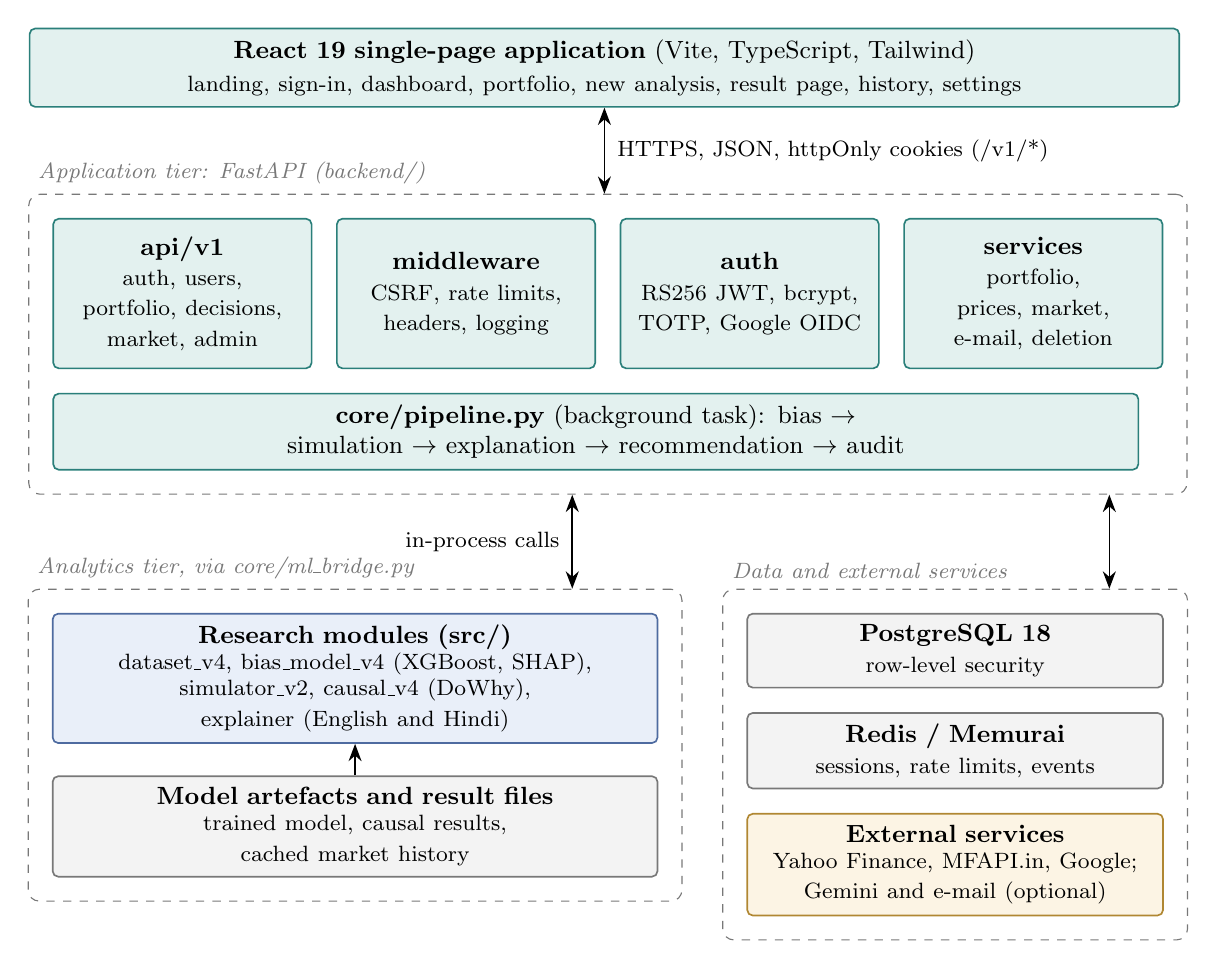
\begin{tikzpicture}
  % Presentation tier
  \node[box, minimum width=146mm, text width=140mm] (spa) {\textbf{React 19 single-page application} (Vite, TypeScript, Tailwind)\\[1pt]
    \footnotesize landing, sign-in, dashboard, portfolio, new analysis, result page, history, settings};

  % Application tier
  \node[box, below=14mm of spa.south west, anchor=north west, xshift=3mm, text width=30mm, minimum height=19mm] (api) {\textbf{api/v1}\\ \footnotesize auth, users, portfolio, decisions, market, admin};
  \node[box, right=3mm of api, text width=30mm, minimum height=19mm] (mw) {\textbf{middleware}\\ \footnotesize CSRF, rate limits, headers, logging};
  \node[box, right=3mm of mw, text width=30mm, minimum height=19mm] (auth) {\textbf{auth}\\ \footnotesize RS256 JWT, bcrypt, TOTP, Google OIDC};
  \node[box, right=3mm of auth, text width=30mm, minimum height=19mm] (svc) {\textbf{services}\\ \footnotesize portfolio, prices, market, e-mail, deletion};
  \node[box, below=3mm of api.south west, anchor=north west, text width=135mm] (pipe)
    {\textbf{core/pipeline.py} (background task): bias $\rightarrow$ simulation $\rightarrow$ explanation $\rightarrow$ recommendation $\rightarrow$ audit};
  \begin{scope}[on background layer]
    \node[tier, fit=(api)(svc)(pipe), inner sep=3mm] (apptier) {};
  \end{scope}
  \node[tierlabel, anchor=south west] at (apptier.north west) {Application tier: FastAPI (backend/)};

  % Analytics tier (left)
  \node[mlbox, below=15mm of apptier.south west, anchor=north west, xshift=3mm, text width=74mm] (src)
    {\textbf{Research modules (src/)}\\ \footnotesize dataset\_v4, bias\_model\_v4 (XGBoost, SHAP),\\ \footnotesize simulator\_v2, causal\_v4 (DoWhy),\\ \footnotesize explainer (English and Hindi)};
  \node[store, below=4mm of src, text width=74mm] (art)
    {\textbf{Model artefacts and result files}\\ \footnotesize trained model, causal results,\\ \footnotesize cached market history};
  \draw[flow] (art) -- (src);
  \begin{scope}[on background layer]
    \node[tier, fit=(src)(art), inner sep=3mm] (mltier) {};
  \end{scope}
  \node[tierlabel, anchor=south west] at (mltier.north west) {Analytics tier, via core/ml\_bridge.py};

  % Data tier (right)
  \node[store, anchor=north east, text width=50mm] (pg) at ($(apptier.south east)+(-3mm,-15mm)$)
    {\textbf{PostgreSQL 18}\\ \footnotesize row-level security};
  \node[store, below=3mm of pg, text width=50mm] (redis)
    {\textbf{Redis / Memurai}\\ \footnotesize sessions, rate limits, events};
  \node[ext, below=3mm of redis, text width=50mm] (ext)
    {\textbf{External services}\\ \footnotesize Yahoo Finance, MFAPI.in, Google;\\ \footnotesize Gemini and e-mail (optional)};
  \begin{scope}[on background layer]
    \node[tier, fit=(pg)(ext), inner sep=3mm] (datatier) {};
  \end{scope}
  \node[tierlabel, anchor=south west] at (datatier.north west) {Data and external services};

  \draw[biflow] (spa.south) -- node[lbl, right=1mm] {HTTPS, JSON, httpOnly cookies (/v1/*)} (spa.south |- apptier.north);
  \draw[biflow] ($(mltier.north east)+(-14mm,0)$) coordinate (m) -- node[lbl, left=1mm] {in-process calls} (m |- apptier.south);
  \draw[biflow] ($(datatier.north east)+(-10mm,0)$) coordinate (d) -- (d |- apptier.south);
\end{tikzpicture}
}
\caption{System architecture of Folium}
\label{fig:arch}
\end{figure}

Figure \ref{fig:arch} shows the overall architecture. The presentation tier is a React single-page application. During development the Vite server forwards every \texttt{/v1/*} request to the API, so the browser sees a single origin, which keeps the httpOnly session cookies and the CSRF check simple.

The application tier is a FastAPI service. Its routes are in \texttt{backend/api/v1/}, its cross-cutting checks in \texttt{backend/middleware/}, its authentication code in \texttt{backend/auth/} and its domain services in \texttt{backend/services/}. The analysis itself runs as a background task under \texttt{backend/core/pipeline.py}.

The analytics tier is the research code in \texttt{src/}. An important design decision is that the back end never re-implements the models. The module \texttt{backend/core/ml\_bridge.py} is the only place where the back end reaches into \texttt{src/}. It imports the heavy ML libraries lazily (they take about two seconds and 400 MB to load), runs blocking work in a worker thread so that the server stays responsive, and maps the vocabulary between the two sides. Since the research modules produced the reported numbers, re-implementing them would risk silently changing those numbers.

PostgreSQL stores users, portfolios, decisions and the audit chain under row-level security. A Redis-compatible store holds the token blacklist, the rate-limit counters and the event backlog for live progress. External services are called only for prices and market data, for Google sign-in, and optionally for e-mail and Gemini.

\section{Analysis Pipeline Components}
\begin{figure}[H]
\centering
\resizebox{0.95\textwidth}{!}{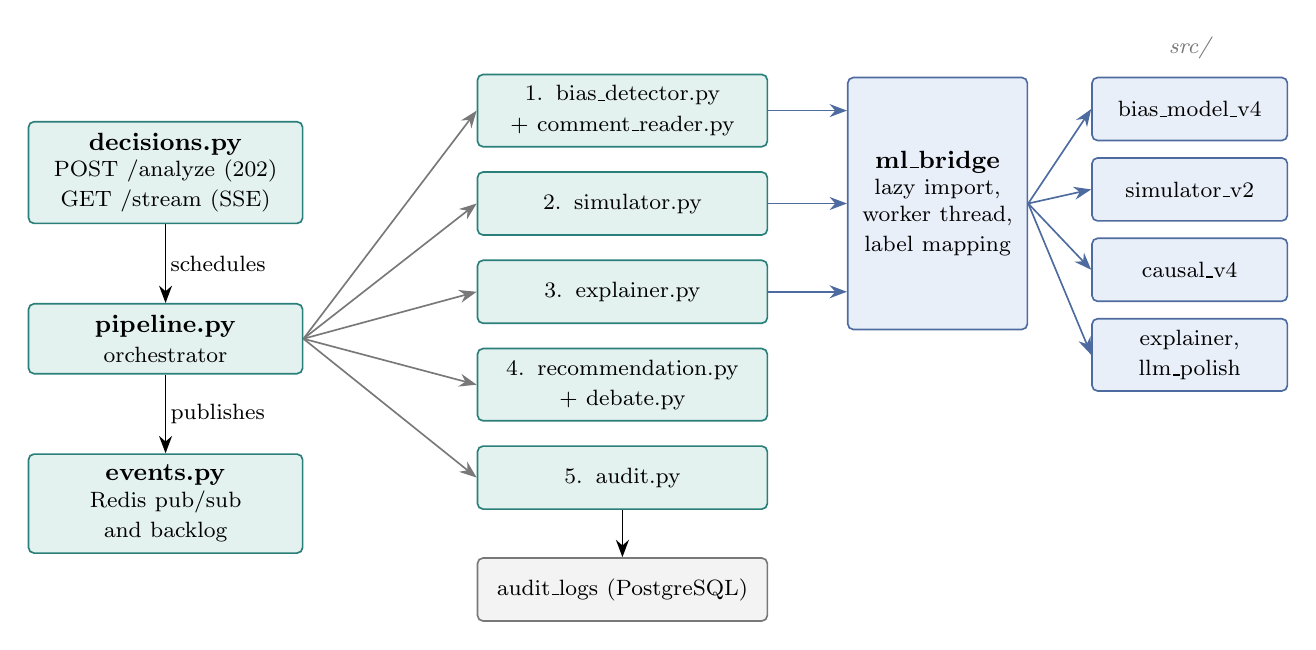
\begin{tikzpicture}[node distance=3mm]
  \node[box, text width=32mm] (dec) {\textbf{decisions.py}\\ \footnotesize POST /analyze (202)\\ \footnotesize GET /stream (SSE)};
  \node[box, below=10mm of dec, text width=32mm] (pipe) {\textbf{pipeline.py}\\ \footnotesize orchestrator};
  \node[box, below=10mm of pipe, text width=32mm] (ev) {\textbf{events.py}\\ \footnotesize Redis pub/sub\\ \footnotesize and backlog};
  \draw[flow] (dec) -- node[lbl, right] {schedules} (pipe);
  \draw[flow] (pipe) -- node[lbl, right] {publishes} (ev);

  \node[box, right=22mm of dec.north east, anchor=north west, text width=34mm, yshift=6mm] (s1) {\footnotesize 1. bias\_detector.py\\ \footnotesize + comment\_reader.py};
  \node[box, below=of s1, text width=34mm] (s2) {\footnotesize 2. simulator.py};
  \node[box, below=of s2, text width=34mm] (s3) {\footnotesize 3. explainer.py};
  \node[box, below=of s3, text width=34mm] (s4) {\footnotesize 4. recommendation.py\\ \footnotesize + debate.py};
  \node[box, below=of s4, text width=34mm] (s5) {\footnotesize 5. audit.py};
  \foreach \s in {s1,s2,s3,s4,s5} \draw[flow, greyline] (pipe.east) -- (\s.west);

  \node[mlbox, right=10mm of s2.east, anchor=west, text width=20mm, minimum height=32mm] (br) {\textbf{ml\_bridge}\\ \footnotesize lazy import,\\ \footnotesize worker thread,\\ \footnotesize label mapping};
  \foreach \s in {s1,s2,s3} \draw[flow, blueline] (\s.east) -- (br.west |- \s.east);

  \node[mlbox, right=8mm of br.north east, anchor=north west, text width=22mm] (m1) {\footnotesize bias\_model\_v4};
  \node[mlbox, below=2mm of m1, text width=22mm] (m2) {\footnotesize simulator\_v2};
  \node[mlbox, below=2mm of m2, text width=22mm] (m3) {\footnotesize causal\_v4};
  \node[mlbox, below=2mm of m3, text width=22mm] (m4) {\footnotesize explainer,\\ \footnotesize llm\_polish};
  \foreach \m in {m1,m2,m3,m4} \draw[flow, blueline] (br.east) -- (\m.west);
  \node[tierlabel, above=1mm of m1] {src/};

  \node[store, below=6mm of s5, text width=34mm] (al) {\footnotesize audit\_logs (PostgreSQL)};
  \draw[flow] (s5) -- (al);
\end{tikzpicture}
}
\caption{Components involved in one analysis}
\label{fig:components}
\end{figure}

Figure \ref{fig:components} shows the components of one analysis. The analyze route (\texttt{POST} on \texttt{/v1/decisions/analyze}) schedules the pipeline as a background task and returns immediately. The orchestrator calls five steps in a fixed order: bias detection, simulation, explanation, recommendation and audit. Each step returns the columns it wants to update and the fields to attach to its progress event, while the orchestrator alone owns the status, the events and persistence. It refuses any step that tries to write the columns it reserves for itself. The first three steps call the research code through the bridge, and the audit step writes to the \texttt{audit\_logs} table.

\section{Data-Flow Diagrams}
\begin{figure}[H]
\centering
\resizebox{0.9\textwidth}{!}{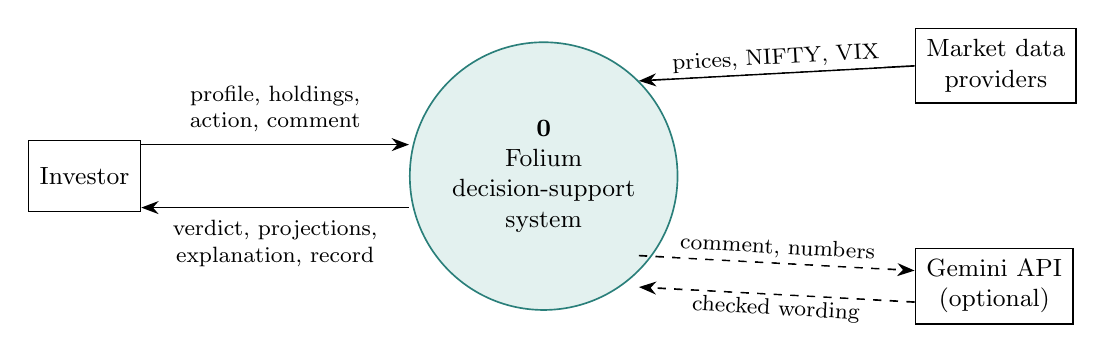
\begin{tikzpicture}
  \node[proc, minimum size=34mm, font=\small] (sys) {\textbf{0}\\ Folium\\ decision-support\\ system};
  \node[entity, left=34mm of sys] (inv) {Investor};
  \node[entity, right=30mm of sys, yshift=14mm] (mkt) {Market data\\ providers};
  \node[entity, right=30mm of sys, yshift=-14mm] (gem) {Gemini API\\ (optional)};
  \draw[flow] ([yshift=4mm]inv.east) -- node[lbl, above=1mm, align=center] {profile, holdings,\\ action, comment} ([yshift=4mm]inv.east -| sys.west);
  \draw[flow] ([yshift=-4mm]inv.east -| sys.west) -- node[lbl, below=1mm, align=center] {verdict, projections,\\ explanation, record} ([yshift=-4mm]inv.east);
  \draw[flow] (mkt.west) -- node[lbl, above, sloped] {prices, NIFTY, VIX} (sys.north east);
  \draw[flow, dashed] ([yshift=2mm]sys.south east) -- node[lbl, above, sloped] {comment, numbers} ([yshift=2mm]gem.west);
  \draw[flow, dashed] ([yshift=-2mm]gem.west) -- node[lbl, below, sloped] {checked wording} ([yshift=-2mm]sys.south east);
\end{tikzpicture}
}
\caption{Data-flow diagram, level 0}
\label{fig:dfd0}
\end{figure}

At the context level (Figure \ref{fig:dfd0}) the system exchanges data with three external entities. The investor supplies a profile, holdings, the intended action and an optional comment, and receives a verdict, projections, an explanation and a verifiable record. Market data providers supply prices, the NIFTY index and the VIX. The Gemini API is optional: it receives a comment and the analysis numbers only when the investor has consented and the server has enabled it, and its output is accepted only after checks.

\begin{figure}[H]
\centering
\resizebox{0.95\textwidth}{!}{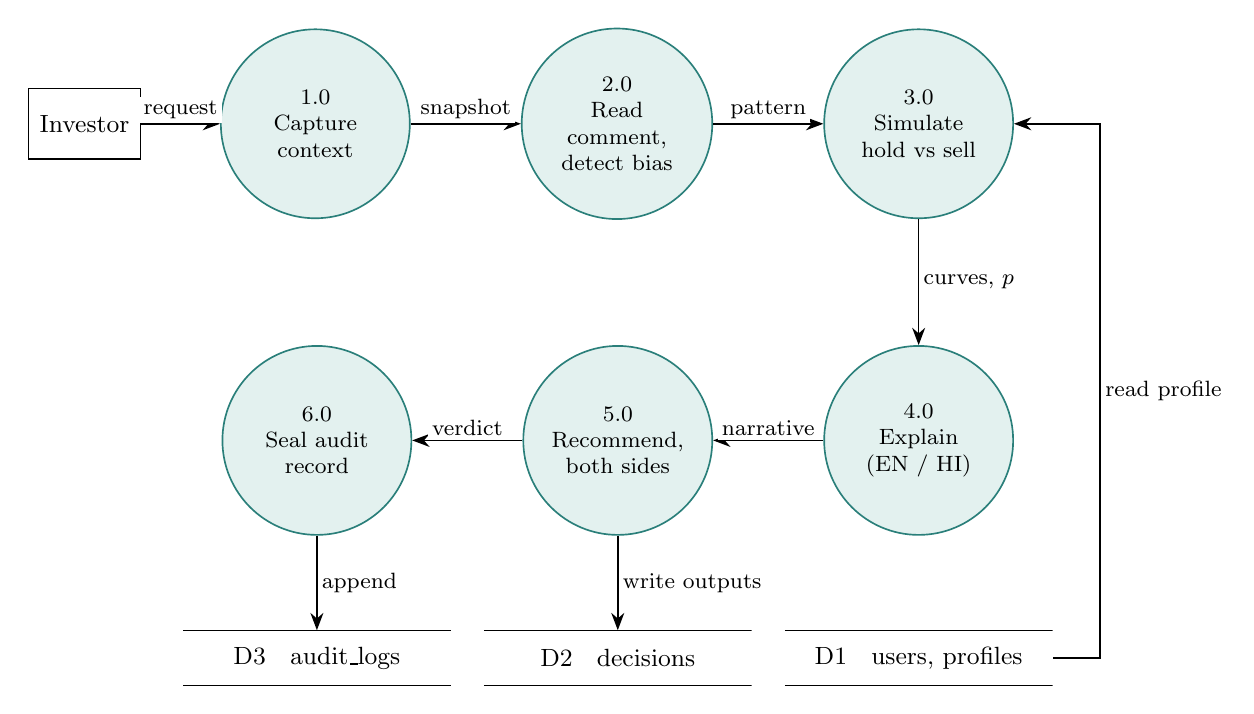
\begin{tikzpicture}[proc/.append style={minimum size=24mm, text width=20mm}]
  \node[proc] (p1) {1.0\\ Capture\\ context};
  \node[proc, right=14mm of p1] (p2) {2.0\\ Read comment,\\ detect bias};
  \node[proc, right=14mm of p2] (p3) {3.0\\ Simulate\\ hold vs sell};
  \node[proc, below=16mm of p3] (p4) {4.0\\ Explain\\ (EN / HI)};
  \node[proc, left=14mm of p4] (p5) {5.0\\ Recommend,\\ both sides};
  \node[proc, left=14mm of p5] (p6) {6.0\\ Seal audit\\ record};
  \node[entity, left=10mm of p1] (inv) {Investor};
  \draw[flow] (inv) -- node[lbl, above] {request} (p1);
  \draw[flow] (p1) -- node[lbl, above] {snapshot} (p2);
  \draw[flow] (p2) -- node[lbl, above] {pattern} (p3);
  \draw[flow] (p3) -- node[lbl, right] {curves, $p$} (p4);
  \draw[flow] (p4) -- node[lbl, above] {narrative} (p5);
  \draw[flow] (p5) -- node[lbl, above] {verdict} (p6);
  \node[datastore, below=12mm of p6] (d3) {D3 \; audit\_logs};
  \node[datastore, below=12mm of p5] (d2) {D2 \; decisions};
  \node[datastore, below=12mm of p4] (d1) {D1 \; users, profiles};
  \draw[flow] (p6) -- node[lbl, right] {append} (d3);
  \draw[flow] (p5) -- node[lbl, right] {write outputs} (d2);
  \draw[flow] (d1.east) -- ++(6mm,0) |- node[lbl, pos=0.25, right] {read profile} (p3.east);
\end{tikzpicture}
}
\caption{Data-flow diagram, level 1 (the analysis process)}
\label{fig:dfd1}
\end{figure}

Figure \ref{fig:dfd1} breaks the analysis into six processes. Process 1.0 is the analyze endpoint, which captures the context, and processes 2.0 to 6.0 are the five pipeline steps. Each process writes its outputs into the decisions store, and the next process reads the refreshed row, which is why the orchestrator reloads the decision before every step. The simulation reads the profile for income, SIP and the destination of sale proceeds, and the last process appends an entry to the audit store.

\section{Use Case Diagram}
\begin{figure}[H]
\centering
\resizebox{0.95\textwidth}{!}{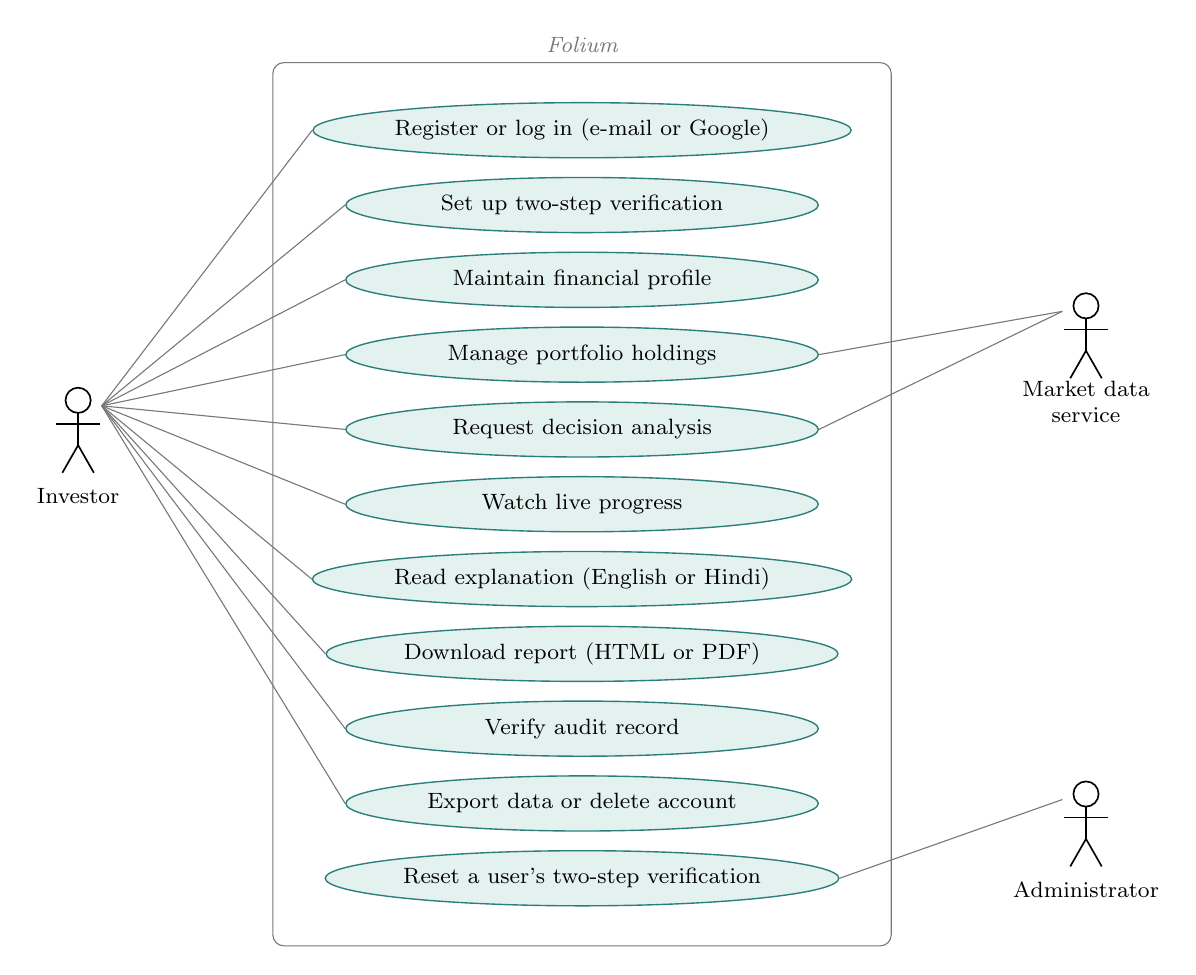
\begin{tikzpicture}
  \foreach \t [count=\i] in {Register or log in (e-mail or Google), Set up two-step verification, Maintain financial profile,
      Manage portfolio holdings, Request decision analysis, Watch live progress, Read explanation (English or Hindi),
      Download report (HTML or PDF), Verify audit record, Export data or delete account, Reset a user's two-step verification}
    \node[usecase] (u\i) at (0,-\i*0.95) {\t};
  \begin{scope}[on background layer]
    \node[draw=greyline, rounded corners=4pt, fit=(u1)(u11), inner sep=5mm] (sysb) {};
  \end{scope}
  \node[tierlabel, anchor=south] at (sysb.north) {Folium};
  \actor{inv}{-6.4,-5.0}{Investor}
  \actor{adm}{6.4,-10.0}{Administrator}
  \actor{mds}{6.4,-3.8}{Market data\\ service}
  \foreach \i in {1,...,10} \draw[greyline] (-6.1,-4.45) -- (u\i.west);
  \draw[greyline] (6.1,-9.45) -- (u11.east);
  \draw[greyline] (6.1,-3.25) -- (u4.east);
  \draw[greyline] (6.1,-3.25) -- (u5.east);
\end{tikzpicture}
}
\caption{Use case diagram}
\label{fig:usecase}
\end{figure}

Figure \ref{fig:usecase} shows the actors and their use cases. The investor can register or log in by e-mail or with Google and then uses every feature of the application. The administrator's implemented use case is resetting a user's two-step verification. The market data service takes part in portfolio management, through live prices, and in analysis requests, through the market context and the stock's measured risk.

\section{Activity Diagram}
\begin{figure}[H]
\centering
\resizebox{0.85\textwidth}{!}{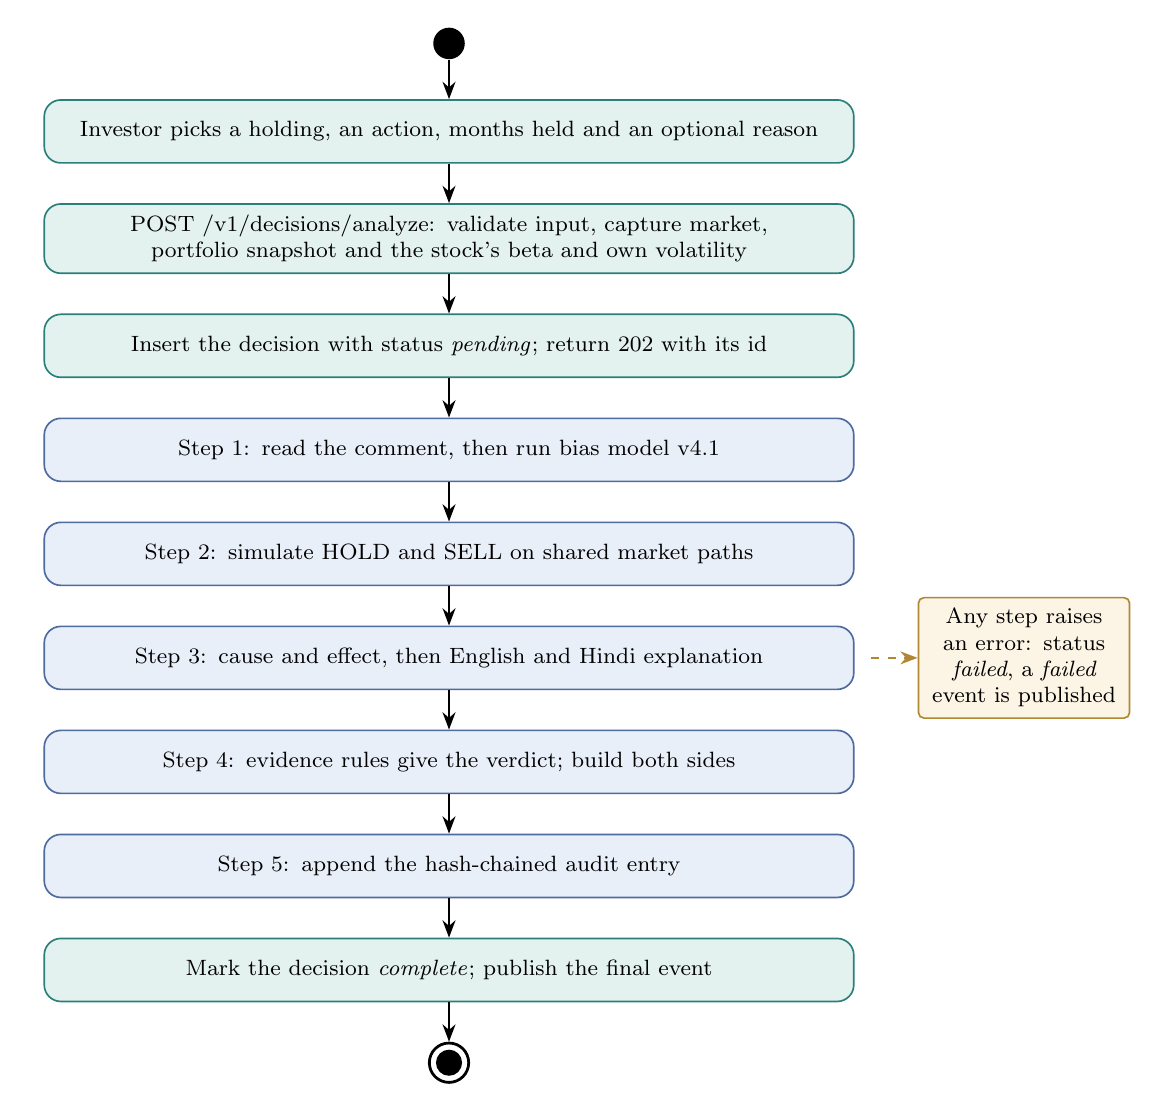
\begin{tikzpicture}[node distance=5mm]
  \node[circle, fill=black, minimum size=4mm] (start) {};
  \node[act, below=of start] (a1) {Investor picks a holding, an action, months held and an optional reason};
  \node[act, below=of a1] (a2) {POST /v1/decisions/analyze: validate input, capture market,\\ portfolio snapshot and the stock's beta and own volatility};
  \node[act, below=of a2] (a3) {Insert the decision with status \emph{pending}; return 202 with its id};
  \node[act, below=of a3, fill=bluefill, draw=blueline] (b1) {Step 1: read the comment, then run bias model v4.1};
  \node[act, below=of b1, fill=bluefill, draw=blueline] (b2) {Step 2: simulate HOLD and SELL on shared market paths};
  \node[act, below=of b2, fill=bluefill, draw=blueline] (b3) {Step 3: cause and effect, then English and Hindi explanation};
  \node[act, below=of b3, fill=bluefill, draw=blueline] (b4) {Step 4: evidence rules give the verdict; build both sides};
  \node[act, below=of b4, fill=bluefill, draw=blueline] (b5) {Step 5: append the hash-chained audit entry};
  \node[act, below=of b5] (c) {Mark the decision \emph{complete}; publish the final event};
  \node[circle, draw=black, line width=1pt, minimum size=5mm, below=of c] (end) {};
  \node[circle, fill=black, minimum size=2.6mm] at (end) {};
  \foreach \x/\y in {start/a1,a1/a2,a2/a3,a3/b1,b1/b2,b2/b3,b3/b4,b4/b5,b5/c,c/end} \draw[flow] (\x) -- (\y);
  \node[box, fill=sandfill, draw=sandline, right=8mm of b3, text width=24mm, font=\footnotesize] (f) {Any step raises an error: status \emph{failed}, a \emph{failed} event is published};
  \begin{scope}[on background layer]
    \node[fit=(b1)(b5), inner sep=2mm] (bg) {};
  \end{scope}
  \draw[flow, dashed, sandline] (bg.east) -- (f.west);
\end{tikzpicture}
}
\caption{Activity diagram of a decision analysis}
\label{fig:activity}
\end{figure}

Figure \ref{fig:activity} traces one analysis. The synchronous part ends with an HTTP 202 response, so the browser never waits for the models. The five shaded steps run in the background. If any step raises an exception, the decision is marked as failed, the error is stored and a failed event is published so that the browser stops waiting. Problems with wording never fail an analysis, because the explanation step falls back to the template text.

\section{Sequence Diagram}
\begin{figure}[H]
\centering
\resizebox{\textwidth}{!}{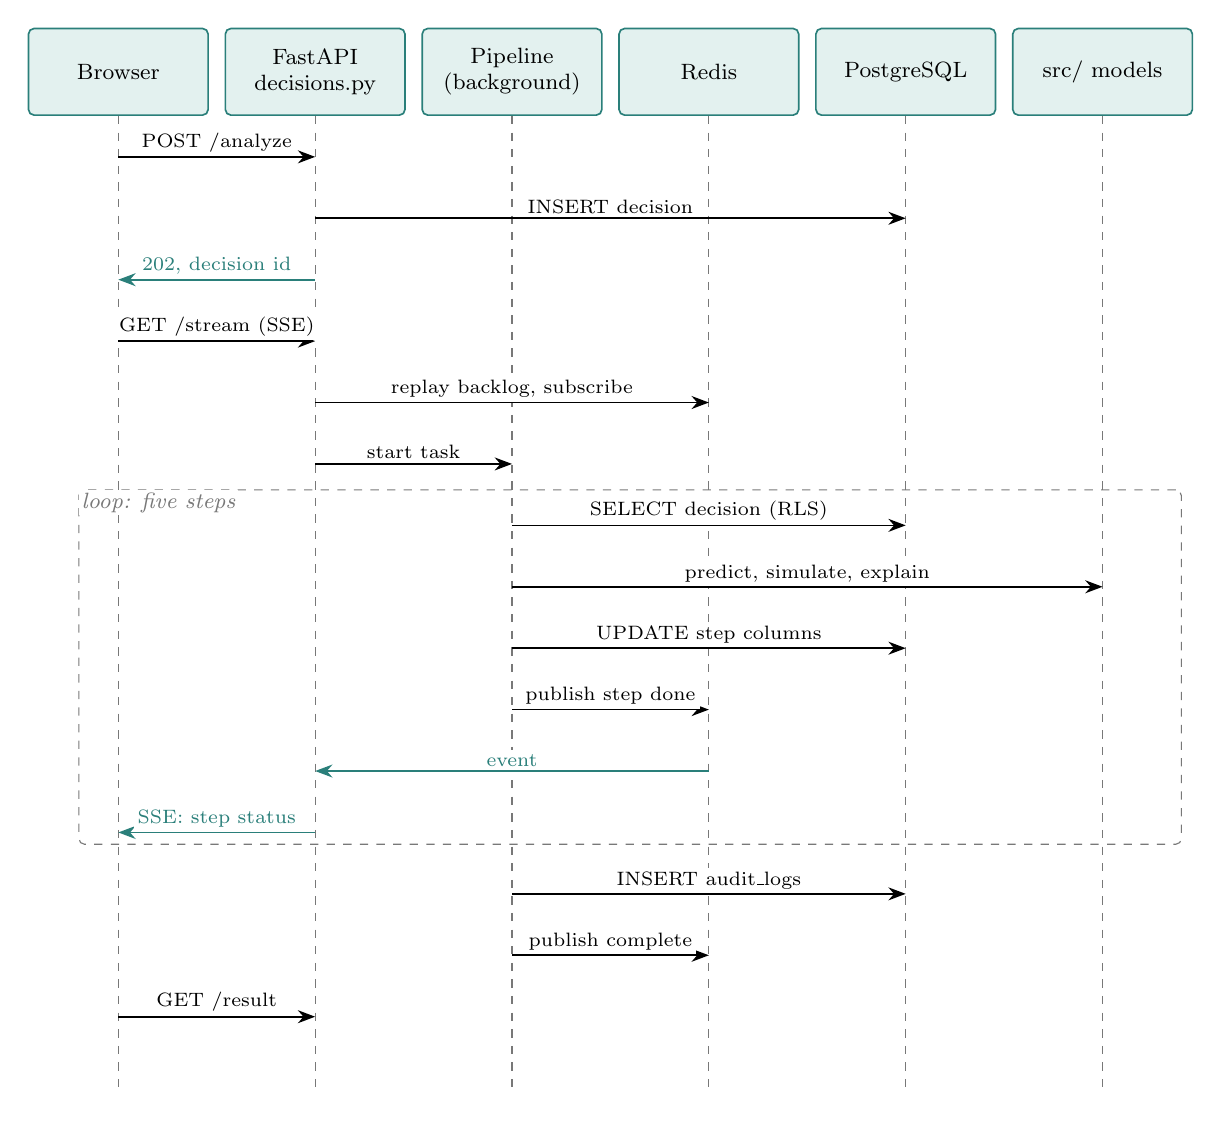
\begin{tikzpicture}
  \foreach \n/\t [count=\i] in {b/Browser, api/{FastAPI\\ decisions.py}, p/{Pipeline\\ (background)}, r/Redis, db/PostgreSQL, m/{src/ models}}
    \node[box, text width=20mm, minimum height=11mm, font=\footnotesize] (\n) at (\i*2.5,0) {\t};
  \foreach \n in {b,api,p,r,db,m} \draw[greyline, dashed] (\n.south) -- ++(0,-12.4);
  \draw[flow, black] (b.south |- 0,-1.08) -- node[lbl, above, font=\scriptsize] {POST /analyze} (api.south |- 0,-1.08);
  \draw[flow, black] (api.south |- 0,-1.86) -- node[lbl, above, font=\scriptsize] {INSERT decision} (db.south |- 0,-1.86);
  \draw[flow, tealline] (api.south |- 0,-2.64) -- node[lbl, above, font=\scriptsize] {202, decision id} (b.south |- 0,-2.64);
  \draw[flow, black] (b.south |- 0,-3.42) -- node[lbl, above, font=\scriptsize] {GET /stream (SSE)} (api.south |- 0,-3.42);
  \draw[flow, black] (api.south |- 0,-4.20) -- node[lbl, above, font=\scriptsize] {replay backlog, subscribe} (r.south |- 0,-4.20);
  \draw[flow, black] (api.south |- 0,-4.98) -- node[lbl, above, font=\scriptsize] {start task} (p.south |- 0,-4.98);
  \draw[flow, black] (p.south |- 0,-5.76) -- node[lbl, above, font=\scriptsize] {SELECT decision (RLS)} (db.south |- 0,-5.76);
  \draw[flow, black] (p.south |- 0,-6.54) -- node[lbl, above, font=\scriptsize] {predict, simulate, explain} (m.south |- 0,-6.54);
  \draw[flow, black] (p.south |- 0,-7.32) -- node[lbl, above, font=\scriptsize] {UPDATE step columns} (db.south |- 0,-7.32);
  \draw[flow, black] (p.south |- 0,-8.10) -- node[lbl, above, font=\scriptsize] {publish step done} (r.south |- 0,-8.10);
  \draw[flow, tealline] (r.south |- 0,-8.88) -- node[lbl, above, font=\scriptsize] {event} (api.south |- 0,-8.88);
  \draw[flow, tealline] (api.south |- 0,-9.66) -- node[lbl, above, font=\scriptsize] {SSE: step status} (b.south |- 0,-9.66);
  \draw[flow, black] (p.south |- 0,-10.44) -- node[lbl, above, font=\scriptsize] {INSERT audit\_logs} (db.south |- 0,-10.44);
  \draw[flow, black] (p.south |- 0,-11.22) -- node[lbl, above, font=\scriptsize] {publish complete} (r.south |- 0,-11.22);
  \draw[flow, black] (b.south |- 0,-12.00) -- node[lbl, above, font=\scriptsize] {GET /result} (api.south |- 0,-12.00);
  \node[draw=greyline, dashed, rounded corners=2pt, fit={(2.0,-5.31) (16.0,-9.81)}, inner sep=0pt] (loop) {};
  \node[tierlabel, anchor=north west, fill=white, inner sep=1pt] at (loop.north west) {loop: five steps};
\end{tikzpicture}
}
\caption{Sequence diagram of an analysis with live progress}
\label{fig:sequence}
\end{figure}

Figure \ref{fig:sequence} shows the order of messages. One detail is the backlog replay. If the browser only subscribed to Redis publish and subscribe, any event published before the subscription would be lost, and reloading the page during an analysis would show an empty history. Every event is therefore also appended to a Redis list with an expiry time. The stream endpoint first replays this list and then follows live messages, removing duplicates by a sequence number. If the stream cannot be opened at all, the result page falls back to polling.

\section{Entity-Relationship Diagram}
\begin{figure}[H]
\centering
\resizebox{0.95\textwidth}{!}{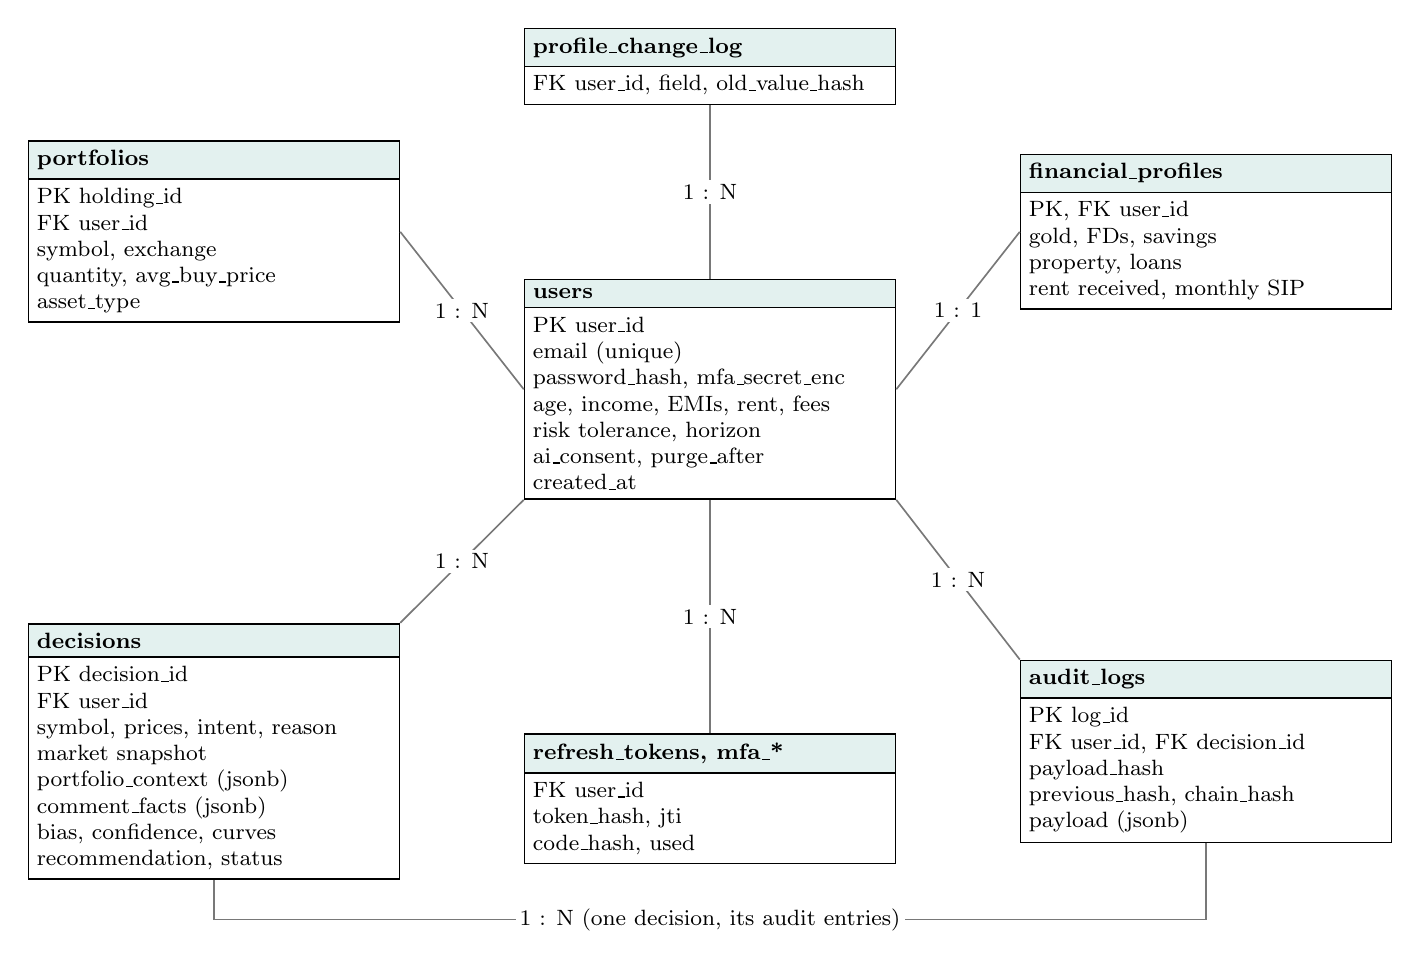
\begin{tikzpicture}[
  ent/.style={rectangle split, rectangle split parts=2, draw=black, line width=0.6pt, align=flush left,
              rectangle split part fill={tealfill, white}, font=\footnotesize\raggedright, inner sep=3pt, text width=45mm},
  rel/.style={draw=greyline, line width=0.6pt}]
  \node[ent] (users) at (0,0) {\textbf{users}\nodepart{two}PK user\_id\\ email (unique)\\ password\_hash, mfa\_secret\_enc\\ age, income, EMIs, rent, fees\\ risk tolerance, horizon\\ ai\_consent, purge\_after\\ created\_at};
  \node[ent] (port) at (-6.3,2.0) {\textbf{portfolios}\nodepart{two}PK holding\_id\\ FK user\_id\\ symbol, exchange\\ quantity, avg\_buy\_price\\ asset\_type};
  \node[ent] (fin) at (6.3,2.0) {\textbf{financial\_profiles}\nodepart{two}PK, FK user\_id\\ gold, FDs, savings\\ property, loans\\ rent received, monthly SIP};
  \node[ent] (dec) at (-6.3,-4.6) {\textbf{decisions}\nodepart{two}PK decision\_id\\ FK user\_id\\ symbol, prices, intent, reason\\ market snapshot\\ portfolio\_context (jsonb)\\ comment\_facts (jsonb)\\ bias, confidence, curves\\ recommendation, status};
  \node[ent] (aud) at (6.3,-4.6) {\textbf{audit\_logs}\nodepart{two}PK log\_id\\ FK user\_id, FK decision\_id\\ payload\_hash\\ previous\_hash, chain\_hash\\ payload (jsonb)};
  \node[ent] (tok) at (0,-5.2) {\textbf{refresh\_tokens, mfa\_*}\nodepart{two}FK user\_id\\ token\_hash, jti\\ code\_hash, used};
  \node[ent] (log) at (0,4.1) {\textbf{profile\_change\_log}\nodepart{two}FK user\_id, field, old\_value\_hash};
  \draw[rel] (users.west) -- node[lbl] {1 : N} (port.east);
  \draw[rel] (users.east) -- node[lbl] {1 : 1} (fin.west);
  \draw[rel] (users.south west) -- node[lbl] {1 : N} (dec.north east);
  \draw[rel] (users.south east) -- node[lbl] {1 : N} (aud.north west);
  \draw[rel] (users.south) -- node[lbl] {1 : N} (tok.north);
  \draw[rel] (users.north) -- node[lbl] {1 : N} (log.south);
  \draw[rel] (dec.south) -- ++(0,-0.5) coordinate (q) -- node[lbl] {1 : N (one decision, its audit entries)} (q -| aud.south) -- (aud.south);
\end{tikzpicture}
}
\caption{Entity-relationship diagram of the main tables}
\label{fig:er}
\end{figure}

Figure \ref{fig:er} shows the main entities, created by Alembic migrations 0001 to 0012. The \texttt{users} table holds the account, the basic financial profile, the deletion schedule and the AI consent flag. \texttt{financial\_profiles} has a one-to-one relationship with users and stores gold, deposits, savings, property, loans, rent received and the monthly SIP, while \texttt{portfolios} holds shares and mutual funds. Each analysis is one row of \texttt{decisions}, which stores both the inputs (including snapshots of the portfolio and the comment reading as JSONB) and every model output. \texttt{audit\_logs} holds the hash-chained entries, and its foreign keys use \texttt{ON DELETE SET NULL} so that the chain survives when an account is anonymized. Row-level security is enabled and forced on decisions, audit logs, portfolios, financial profiles and the profile change log.

\section{Deployment Diagram}
\begin{figure}[H]
\centering
\resizebox{0.9\textwidth}{!}{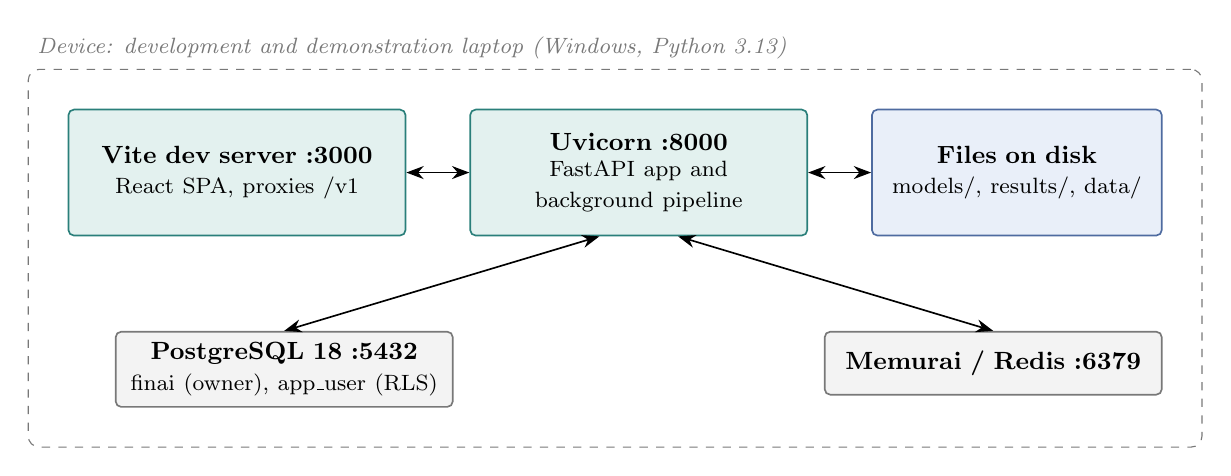
\begin{tikzpicture}
  \node[box, text width=40mm, minimum height=16mm] (vite) {\textbf{Vite dev server :3000}\\ \footnotesize React SPA, proxies /v1};
  \node[box, right=8mm of vite, text width=40mm, minimum height=16mm] (uv) {\textbf{Uvicorn :8000}\\ \footnotesize FastAPI app and\\ \footnotesize background pipeline};
  \node[mlbox, right=8mm of uv, text width=34mm, minimum height=16mm] (art) {\textbf{Files on disk}\\ \footnotesize models/, results/, data/};
  \node[store, below=12mm of uv.south west, anchor=north east, xshift=-2mm, text width=40mm] (pg) {\textbf{PostgreSQL 18 :5432}\\ \footnotesize finai (owner), app\_user (RLS)};
  \node[store, below=12mm of uv.south east, anchor=north west, xshift=2mm, text width=40mm] (rd) {\textbf{Memurai / Redis :6379}};
  \draw[biflow] (vite) -- (uv);
  \draw[biflow] (uv) -- (art);
  \draw[biflow] (uv.south) ++(-5mm,0) -- (pg.north);
  \draw[biflow] (uv.south) ++(5mm,0) -- (rd.north);
  \begin{scope}[on background layer]
    \node[tier, fit=(vite)(art)(pg)(rd), inner sep=5mm] (dev) {};
  \end{scope}
  \node[tierlabel, anchor=south west] at (dev.north west) {Device: development and demonstration laptop (Windows, Python 3.13)};
\end{tikzpicture}
}
\caption{Deployment diagram of the development set-up}
\label{fig:deploy}
\end{figure}

Figure \ref{fig:deploy} shows the configuration used for development and demonstration, with all processes on one laptop. PostgreSQL has two roles: \texttt{finai}, the owner used for migrations, and \texttt{app\_user}, a non-superuser used by the application so that the row-level security policies apply. Container definitions are present in the repository for the planned public deployment.

\section{User Interface Design}
The public pages are the landing page, the privacy policy and the sign-in pages, together with \texttt{/auth/google}, where Google sign-in returns. A first Google sign-in lands on a Welcome page that asks for the basic profile; until it is filled, every other signed-in page except Settings sends the investor there. The application pages are an overview dashboard, the portfolio, a new-analysis form with a live market card, the result page, the history and the settings.

The result page is the centre of the design. It shows the live five-step progress with plain titles such as ``Reading your decision'' and ``Projecting the future'', then the recommendation with its reasons, the position against the whole portfolio, a chart of both futures, the pattern found with probability bars, the six-part explanation with an English and Hindi switch, report downloads, the inputs that weighed most, cause and effect, both sides in numbers, the investor's own words, ``Verify this record'' and ``How this was worked out''. The interface never shows a model name or an accuracy figure, and confidence is shown in words.

\chapter{Methodology}
Folium treats an investment decision as the unit of analysis. The investor states what they intend to do with one holding, and the system answers separate questions before combining them: which pattern is most likely behind the decision (the bias model), what each choice would lead to in rupees after tax over the investor's horizon (the simulator), what generally pushes people towards this action and which habit would help (the causal module), and what the investor should do and why (the evidence rules and the explanation engine). Keeping these questions apart is the main methodological choice of the project. Each module reports only what it can support, and the recommendation rules read only the outputs they are designed to read.

The work has an offline part and an online part. Offline, the dataset is built from real market history, the bias model is trained and evaluated, and the simulator and causal module are evaluated; the outputs are model artefacts and result files. Online, for each analysis, the request and its context are captured and the five pipeline steps run. The online path only loads the offline artefacts and never retrains anything.

\section{Data Sources}
Three kinds of data are used. Daily NIFTY 50 closes and India VIX values \cite{b54} were downloaded through yfinance \cite{b52} and cached (10 June 2008 to 5 October 2026, 4,475 trading days). Monthly NIFTY 50 returns, with a 1.25\% dividend yield added, and gold returns in rupees from October 2007 to September 2026 (228 months) are cached for the simulator. Second, the synthetic investor decisions of dataset v4.1 are used for training and causal validation. Third, live share prices, mutual fund NAVs from MFAPI.in \cite{b53} and the gold price are fetched at run time and cached for 15 minutes. No real investor's trading records are used.

\section{Dataset v4.1}
There is no public dataset that links the individual decisions of Indian retail investors with their full finances and a ground-truth behavioral label, and building one would require a large consented user study. The decisions are therefore generated synthetically while the market side is kept real. The design principle is that labels are motives and not rules. Each simulated investor has hidden tendencies, the situation decides which biased motives are possible, these compete with a rational motive, and the winning motive decides both the action and the label. The same sale can therefore be rational for one investor and biased for another, and the model has to infer which from what the app can observe.

\begin{figure}[H]
\centering
\resizebox{\textwidth}{!}{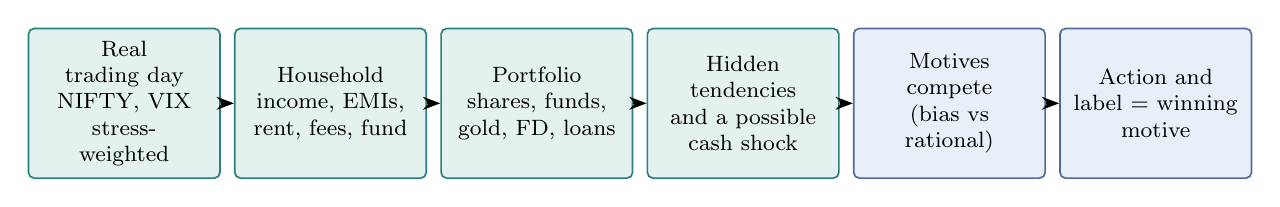
\begin{tikzpicture}[node distance=4mm]
  \foreach \t [count=\i] in {{Real trading day\\ NIFTY, VIX\\ stress-\\ weighted}, {Household\\ income, EMIs,\\ rent, fees, fund}, {Portfolio\\ shares, funds,\\ gold, FD, loans}, {Hidden tendencies\\ and a possible\\ cash shock}, {Motives\\ compete\\ (bias vs rational)}, {Action and\\ label = winning\\ motive}}
    \node[box, text width=21.5mm, minimum height=19mm, font=\footnotesize, fill=\ifnum\i>4 bluefill\else tealfill\fi, draw=\ifnum\i>4 blueline\else tealline\fi] (d\i) at (\i*2.62,0) {\t};
  \foreach \i [evaluate=\i as \j using int(\i+1)] in {1,...,5} \draw[flow] (d\i) -- (d\j);
\end{tikzpicture}
}
\caption{Generation of one case in dataset v4.1}
\label{fig:datasetgen}
\end{figure}

Figure \ref{fig:datasetgen} shows the steps. A real trading day is sampled with stress over-weighted (weights of 1 for normal and bull days, 2 for corrections, 3 for euphoria and 6 for crashes) so that every motive has enough examples, and the day's real one-month return, volatility, VIX and 52-week drawdown are attached. A holding period is drawn from a log-normal distribution with a median of 14 months, and the gain or loss on the position is the real NIFTY move over that period raised to a stock beta, plus stock-specific noise. A household is then generated with age, income, years of investing, risk tolerance, horizon, rent, EMIs, education fees and an emergency fund; 14\% of borrowers carry extra debt worth 25 to 65\% of income. A portfolio of shares, funds, gold, deposits, savings, property and loans follows. Hidden tendencies are drawn, and a cash shock (job loss, medical bill or fees due) occurs with probability
\begin{equation}
P(\text{shock}) = 0.04 + 0.06\,[\text{no fund}] + 0.12\,\mathrm{clip}\!\left(\frac{0.30 - s}{0.30}, 0, 1\right),
\end{equation}
where $s$ is the surplus ratio. An emergency fund absorbs 70\% of shocks. Investors who genuinely need the money say so with probability 0.65, and others mention it with probability 0.03; this is the observable input \texttt{cash\_need\_stated}.

\begin{table}[H]
\centering
\small
\begin{tabularx}{\textwidth}{|P{2.4cm}|P{2.4cm}|P{1.6cm}|L|}
\hline
\textbf{Label} & \textbf{Motive} & \textbf{Action} & \textbf{Applies when} \\
\hline
Loss aversion & panic & sell & at a loss, NIFTY down 2\% or more over the month, and VIX $\geq$ 20 or a correction or crash \\
\hline
Loss aversion & refusal & hold & position down 25\% or more \\
\hline
Disposition effect & sell a winner & sell & up 8\% or more in a normal or rising market \\
\hline
Disposition effect & hold a loser & hold & down 5 to 25\% in a normal or rising market \\
\hline
Herd behavior & sell into fear & sell & VIX $\geq$ 22 or NIFTY down 5\% or more over the month \\
\hline
Herd behavior & buy into a rally & buy more & NIFTY up 4\% or more over the month \\
\hline
Rational & stay the course, add regularly, buy value, average down, cut a loss, rebalance, goal near, needs cash & any & the investor's own situation explains the action \\
\hline
\end{tabularx}
\caption{Label definitions used by the generator}
\label{tab:labels}
\end{table}

For a case with situation $s$ and investor $i$, the rational motive competes with weight
\begin{equation}
w_r = 0.7 + 0.025\,y_i + 0.25\,e_i + 3.0\,c_i ,
\end{equation}
where $y_i$ is years of investing, $e_i$ indicates an emergency fund and $c_i$ indicates that the money is genuinely needed. A bias motive $m$ with label $\ell$ competes with weight $w_m = S_\ell\,\tau_{i,\ell}^{1.5}\,I_m(s)$, where $\tau_{i,\ell}$ is the hidden tendency, $S_\ell$ is 3.4 for loss aversion, 2.0 for herding and 2.8 for disposition, and $I_m(s) \geq 1$ is the intensity of the situation. One motive is sampled in proportion to its weight. The large weight for a genuine cash need encodes the idea that necessity is a constraint and not a preference.

\begin{figure}[H]
\centering
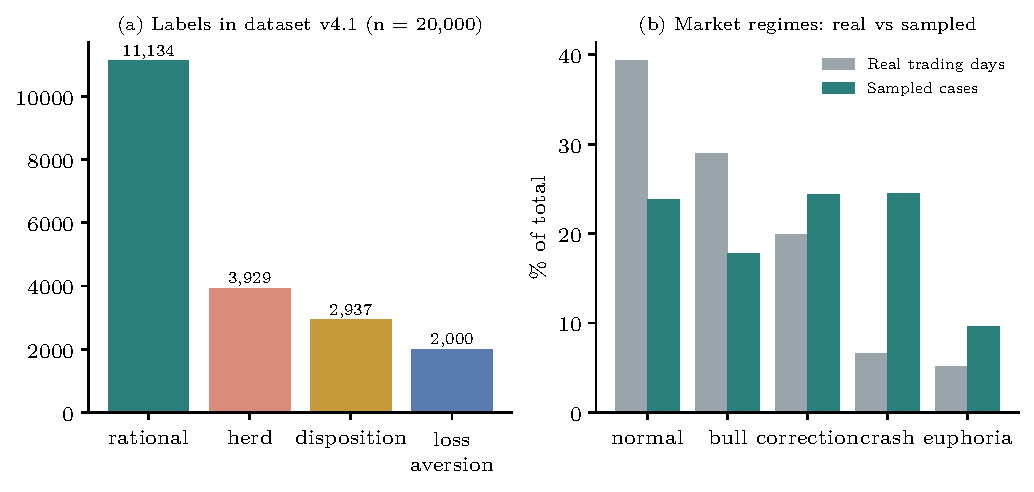
\includegraphics[width=0.95\textwidth]{figures/charts/dataset_distribution.pdf}
\caption{(a) Label distribution in dataset v4.1; (b) market regimes among real trading days and sampled cases}
\label{fig:datadist}
\end{figure}

The dataset has 20,000 cases (Figure \ref{fig:datadist}): 11,134 rational (55.7\%), 3,929 herd (19.6\%), 2,937 disposition (14.7\%) and 2,000 loss aversion (10.0\%), with 8,251 holds, 7,995 sales and 3,754 purchases. Crashes form 24.5\% of the cases against 6.6\% of real days, so every evaluation figure is re-weighted back to real regime frequencies. The median investor is 38 years old with a monthly income of \rupee 75,000 and liquid assets of \rupee 9.7 lakh, and the median position is 12\% of liquid assets. Money pressure is represented explicitly: 0.7\% of households pay out more than they earn, 44\% have no emergency fund, cash shocks hit 6.8\% of decisions, and the money is needed in 1,165 cases, 889 of which end in a forced sale.

\section{Feature Engineering}
The same function converts raw inputs into the 22 model features for training and for live requests, so the two cannot drift apart. Besides three action flags, the gain or loss, holding period, market values, age, horizon, risk tolerance and portfolio shares, two ratios are derived:
\begin{align}
\text{surplus ratio} &= \mathrm{clip}\!\left(\frac{\text{income} + \text{rent received} - \text{fixed outflow}}{\text{income}}, -2, 2\right),\\
\text{debt ratio} &= \mathrm{clip}\!\left(\frac{\text{loans}}{\text{liquid assets} + \text{property}}, 0, 5\right).
\end{align}
Three \texttt{allows} flags state which biased labels the definitions permit for this situation and action. In the product, missing profile fields are filled with training medians and missing market data with the median real trading day (NIFTY up 1.0\% in a month, VIX 16.9); all filled values are listed on the result page.

\section{Behavioral Classification}
Let $\mathbf{x} \in \mathbb{R}^{22}$ be the feature vector and $y \in \{1,\dots,K\}$ with $K = 4$. The boosted-tree score for class $k$ and its probability are
\begin{equation}
F_k(\mathbf{x}) = \sum_{m=1}^{M} f_{m,k}(\mathbf{x}), \qquad \hat{p}_k(\mathbf{x}) = \frac{e^{F_k(\mathbf{x})}}{\sum_{j=1}^{K} e^{F_j(\mathbf{x})}} ,
\end{equation}
and the training objective combines the weighted log-loss with a penalty on tree complexity \cite{b5,b26}:
\begin{equation}
\mathcal{L} = \sum_{i=1}^{n} w_i\,\ell\big(y_i, \hat{\mathbf{p}}(\mathbf{x}_i)\big) + \sum_{m,k} \Omega(f_{m,k}), \qquad \Omega(f) = \gamma T + \tfrac{1}{2}\lambda \lVert \boldsymbol{\omega} \rVert^2 ,
\end{equation}
where $T$ is the number of leaves, $\boldsymbol{\omega}$ the leaf weights and $w_i$ the ratio of the real to the sampled frequency of the case's regime.

\textbf{Guard.} Let $m_k(\mathbf{x}) = 1$ if label $k$ is allowed by the definitions, with the rational label always allowed. The guarded probabilities are $\tilde{p}_k = m_k\hat{p}_k / \sum_j m_j \hat{p}_j$, so the model can never output a pattern the definitions rule out.

\textbf{Calibration.} Let $c$ be the probability of the chosen class. A centered isotonic regression \cite{b47} fitted on out-of-fold predictions maps $c$ to a calibrated value; unlike plain isotonic regression, which is a step function, it joins the weighted centers of the constant blocks with straight lines. The calibrated value is floored so that the chosen class can never fall below the runner-up, and is capped at 0.99. Calibration is measured by the expected calibration error over ten confidence bins:
\begin{equation}
\mathrm{ECE} = \sum_{b=1}^{10} \frac{W(B_b)}{W}\,\big|\mathrm{acc}(B_b) - \mathrm{conf}(B_b)\big| .
\end{equation}
The confidence is shown to the investor as High (0.85 and above), Medium (0.65 and above) or Low.

\textbf{Attribution.} For the chosen class, SHAP decomposes the score additively, $F_k(\mathbf{x}) = \phi_{0,k} + \sum_{j} \phi_{j,k}(\mathbf{x})$ \cite{b7}, and exact TreeSHAP values \cite{b35} are summed into 18 plain drivers such as ``gain or loss'' or ``market fear''. Because Shapley values are additive this grouping is exact; the largest additivity error on the evaluation checks is $8.1\times10^{-6}$.

\section{Paired Hold versus Sell Simulation}
Let $r^E_t$ and $r^G_t$ be the monthly log-returns of NIFTY 50 and of gold in rupees. To keep the swings of history but set typical growth to stated long-run rates ($\mu_E = 11\%$, $\mu_G = 9\%$), each series is re-centered,
\begin{equation}
\tilde{r}^E_t = r^E_t - \bar{r}^E + \frac{\ln(1+\mu_E)}{12}, \qquad \tilde{r}^G_t = r^G_t - \bar{r}^G + \frac{\ln(1+\mu_G)}{12}.
\end{equation}
A path of $12H$ months is built from 12-month blocks whose starting months are drawn uniformly, with indices taken modulo the history length (a circular block bootstrap \cite{b12,b33}). The same indices are used for equity and gold, which keeps their real month-by-month relationship. Re-centering is needed because gold compounded at about 14.8\% a year from 2007 to 2026, and replaying that as the future would build an unusually strong gold boom into every path.

For a stock with beta $\beta$ and company-specific monthly volatility $\sigma$, the typical growth follows the capital asset pricing relation with the fixed deposit rate $r_f = 6.75\%$, $\mu_{\text{pos}} = r_f + \beta(\mu_E - r_f)$, and the monthly log-return on path $s$ is
\begin{equation}
\rho_{s,t} = \frac{\ln(1+\mu_{\text{pos}})}{12} + \beta\big(\tilde{r}^E_{s,t} - \bar{\tilde{r}}^E\big) + \varepsilon_{s,t}, \qquad \varepsilon_{s,t} \sim \mathcal{N}\!\left(-\tfrac{\sigma^2}{2}, \sigma^2\right).
\end{equation}
With $V_0$ the value today, $C$ the cost basis, $\kappa = 0.15\%$ the sale charges and $m_0$ the months already held, the value in hand after holding for $t$ months is
\begin{equation}
W^{(H)}_{s,t} = V_t (1-\kappa) - \mathrm{Tax}_E\big(V_t - C,\; m_0 + t\big), \qquad V_t = V_0\, e^{\sum_{u \leq t} \rho_{s,u}} .
\end{equation}
Selling realizes $P = V_0 - \mathrm{Tax}_E(V_0 - C, m_0) - \kappa V_0$ today and moves it into the investor's existing mix of gold, deposits and savings, with shares $\alpha_G, \alpha_F, \alpha_S$:
\begin{equation}
W^{(S)}_{s,t} = \alpha_G P\,G_{s,t} - \mathrm{Tax}_G(\cdot) + \alpha_F P\big(1 + r_f(1-\tau)\big)^{t/12} + \alpha_S P\big(1 + r_{sv}(1-\tau)\big)^{t/12},
\end{equation}
where $\tau$ is the investor's marginal slab rate on interest and $r_{sv} = 3\%$. Because both values are computed on the same path, their difference isolates the decision. The outputs are
\begin{align}
\tilde{\Delta}_T &= \mathrm{median}_s \big(W^{(H)}_{s,T} - W^{(S)}_{s,T}\big),\\
p &= \frac{1}{n}\sum_{s=1}^{n} \mathbf{1}\big[W^{(H)}_{s,T} > W^{(S)}_{s,T}\big],
\end{align}
together with the 10th, 50th and 90th percentiles of both paths for every year. The median is used because single-stock outcomes are right-skewed, so the mean would overstate the usual result.

\begin{table}[H]
\centering
\small
\begin{tabularx}{\textwidth}{|P{4.4cm}|L|}
\hline
\textbf{Item} & \textbf{Rule (FY 2025-26, new regime)} \\
\hline
Listed equity held 12 months or less & 20\% short-term gains tax \\
\hline
Listed equity held longer & 12.5\% on gains above \rupee 1,25,000 \\
\hline
Gold & 12.5\% after 24 months; otherwise the slab rate \\
\hline
FD and savings interest & The investor's marginal slab rate, every year \\
\hline
Cess & 4\% on top of each tax \\
\hline
Slab rate & Taxable income is gross minus \rupee 75,000; nil up to \rupee 12 lakh taxable (Section 87A rebate); above that slabs of 0, 5, 10, 15, 20, 25 and 30\% in steps of \rupee 4 lakh \\
\hline
\end{tabularx}
\caption{Tax rules used by the simulator}
\label{tab:tax}
\end{table}

The tax rules in Table \ref{tab:tax} follow the Finance (No. 2) Act, 2024 \cite{b55} and the Finance Act, 2025 \cite{b56}. The slab rate depends on income before tax, but the app records take-home pay. If $T(g)$ is the income tax on gross income $g$, including the rebate and its marginal relief, then take-home pay is $h(g) = g - T(g)$, and the simulator needs $\hat{g}$ such that $h(\hat{g})$ equals twelve times the monthly take-home pay. Since $h$ is increasing except in a short stretch of the marginal relief band, $\hat{g}$ is found by bisection with 60 iterations, and rent received is added at 70\%. For example, a take-home pay of \rupee 1.6 lakh a month corresponds to about \rupee 21.5 lakh gross, so interest is taxed at 26\% and not the 20.8\% that the take-home figure alone would give.

\section{Causal Estimation}
For a treatment $A$ and an outcome $Y$ (whether the investor takes a given action), the average treatment effect and its identification by the g-formula under consistency, positivity and conditional exchangeability given an adjustment set $Z$ are \cite{b10,b36,b37}
\begin{align}
\mathrm{ATE} &= \mathbb{E}[Y \mid \mathrm{do}(A = a')] - \mathbb{E}[Y \mid \mathrm{do}(A = a)],\\
\mathbb{E}[Y \mid \mathrm{do}(A = a)] &= \sum_{z} \mathbb{E}[Y \mid A = a, Z = z]\,P(Z = z).
\end{align}
Two estimators work from the data alone, as a real study would. G-computation fits a histogram gradient-boosting model of the action given everything observed (scikit-learn \cite{b48}, 400 iterations) and averages its predictions with the treatment set to each value. DoWhy \cite{b11} identifies the effect from a graph that mirrors the generator and estimates it with a linear model, followed by placebo, random common cause and subset refutation tests.

Because the generator is known exactly, the true effect can also be computed by re-evaluating the generator's motive probabilities with the input changed. This is what makes the evaluation possible: the estimates can be compared with the truth, which is never available in a real observational study. Gold share has no causal path to the decision and is used as a negative control. A habit is modeled as halving the tendency it acts on, which is an assumption stated in the app.

\section{Evidence-Based Recommendation}
\begin{table}[H]
\centering
\small
\begin{tabularx}{\textwidth}{|P{2.2cm}|L|}
\hline
\textbf{Intent} & \textbf{Rule} \\
\hline
Sell & $p \geq 0.60$ gives HOLD; $p \leq 0.40$ gives SELL; otherwise HOLD if the sale reads as biased, else SELL \\
\hline
Hold & $p \leq 0.40$ gives SELL; otherwise HOLD \\
\hline
Buy more & Herd behavior, or any bias with confidence $\geq 0.60$, gives HOLD; otherwise BUY MORE if $p \geq 0.50$, else HOLD \\
\hline
\end{tabularx}
\caption{Recommendation rules}
\label{tab:rules}
\end{table}

The verdict comes from the small rule set in Table \ref{tab:rules}, where $p$ is the share of simulated futures in which holding beats selling. The band between 0.40 and 0.60 is treated as a toss-up, in which the behavioral reading decides. A verdict about money should be checkable by hand, and a rule set with stated thresholds meets this need where a language model would not. Every verdict stores its reasons and the exact numbers used.

\section{Explanation}
All model outputs are gathered into one dictionary of facts. Hand-written Jinja2 \cite{b57} templates, identical in structure in English and Hindi, turn the facts into six sections: in short, what is going on right now, your two possible futures, the story of your money, why we are telling you this, and what to do now. An optional Gemini rewording is accepted only if it introduces no new number or rupee amount and its length stays between 0.6 and 1.8 times the original.

\section{Tamper-Evident Audit Chain}
Let $\mathrm{canon}(\cdot)$ be a canonical JSON serialization (sorted keys, no spaces) and $H$ be SHA-256. For the $i$-th entry of an investor, with payload $P_i$,
\begin{align}
h_0 &= H(\texttt{GENESIS:} \Vert \text{user id} \Vert \texttt{:} \Vert \text{created at}),\\
\pi_i &= H(\mathrm{canon}(P_i)), \qquad h_i = H(h_{i-1} \Vert \pi_i).
\end{align}
Changing any byte of a payload changes $\pi_i$ and therefore every later chain hash, and removing an entry leaves the next one pointing at a hash that no entry produces, following the linked time-stamping idea of Haber and Stornetta \cite{b44}. Verification walks the entries by following the links from the genesis value rather than by timestamp, and reports an entry as altered if its hashes do not recompute, as unlinked if it does not connect to the chain, and as a fork if two entries claim the same predecessor.

\chapter{Implementation}
This chapter describes the implementation module by module. The code listings are excerpts copied from the repository; omitted lines are marked with \texttt{...}, and identifiers and logic are unchanged.

\begin{table}[H]
\centering
\small
\begin{tabularx}{\textwidth}{|P{2.6cm}|L|}
\hline
\textbf{Path} & \textbf{Contents} \\
\hline
\texttt{backend/} & Product API: routes, authentication, the analysis pipeline and its steps, services, database layer and migrations, middleware and tests \\
\hline
\texttt{frontend/} & React application: pages, components, API client, query hooks and tests \\
\hline
\texttt{src/} & Models and engines: dataset generator, bias model, simulator, causal module, explainer and templates; earlier versions kept for rollback \\
\hline
\texttt{models/}, \texttt{data/} & Trained model files; the dataset and cached market history \\
\hline
\texttt{results/}, \texttt{scripts/} & Evaluation files and reports; training, evaluation and maintenance scripts \\
\hline
\texttt{tests/}, \texttt{notebooks/} & Tests for the models and engines; research notebooks \\
\hline
\end{tabularx}
\caption{Organization of the repository}
\label{tab:repo}
\end{table}

\section{Dataset Generator}
The generator in \texttt{src/dataset\_v4.py} produces the 20,000 labelled decisions. Its most important function for the rest of the system is \texttt{applicable\_bias\_motives}, which encodes the label table, together with \texttt{allowed\_labels}, which the bias model uses both as an input and as a guard. Keeping the table in one place means that the generator, the model and the tests cannot disagree about what a label means.

\begin{lstlisting}[caption={The label rules in code form (\texttt{src/dataset\_v4.py})}, label=lst:rules]
def applicable_bias_motives(s: dict) -> list[Motive]:
    gl, r1m, vix, regime = s["unrealized_gl"], s["nifty_1m_return"], s["vix"], s["regime"]
    falling_fear = gl < -0.03 and r1m <= FALLING_1M and (vix >= FEAR_VIX or regime in ("crash", "correction"))
    calm = regime in ("normal", "bull")
    out: list[Motive] = []
    if falling_fear:
        out.append(Motive("loss_aversion_panic", "loss_aversion", "sell"))
    if gl <= DEEP_LOSS:
        out.append(Motive("loss_aversion_refusal", "loss_aversion", "hold"))
    if calm and gl >= EARLY_WIN:
        out.append(Motive("disposition_sell_winner", "disposition", "sell"))
    if calm and DEEP_LOSS < gl <= MODERATE_LOSS:
        out.append(Motive("disposition_hold_loser", "disposition", "hold"))
    if vix >= HERD_FEAR_VIX or r1m <= HERD_FEAR_1M:
        out.append(Motive("herd_sell_fear", "herd", "sell"))
    if r1m >= FRENZY_1M:
        out.append(Motive("herd_buy_frenzy", "herd", "buy_more"))
    return out
\end{lstlisting}

The thresholds are module constants, so the dataset card, the tests and the code all refer to the same values. Using \texttt{numpy.random.default\_rng(2026)} with the cached market file makes the dataset identical on every rebuild.

\section{Bias Model}
\texttt{src/bias\_model\_v4.py} builds the features, loads the model and makes predictions. The function \texttt{build\_features} refuses to run with missing inputs or an unknown action, so that the caller fills any gap and can disclose what it filled. The model is stored as native XGBoost JSON with a metadata file that holds the feature list, the calibration curve and the training medians, and \texttt{load} refuses to run if the stored feature list differs from the code.

\begin{lstlisting}[caption={The definitional guard and top-label calibration (\texttt{src/bias\_model\_v4.py})}, label=lst:calib]
def apply_guard(p: np.ndarray, mask: np.ndarray) -> np.ndarray:
    """Zero the patterns the definitions rule out, then renormalise."""
    q = p * mask
    return q / q.sum(axis=1, keepdims=True)

def calibrate_top_label(p, curve_x, curve_y):
    p = np.asarray(p, dtype=float)
    k = p.argmax(axis=1)
    rows = np.arange(len(p))
    top = p[rows, k]
    rest = 1.0 - top
    second = np.sort(p, axis=1)[:, -2]
    c = np.interp(top, curve_x, curve_y)
    floor = np.where(rest > 0, second / np.maximum(rest + second, 1e-12) + 1e-6, top)
    c = np.clip(np.maximum(c, floor), 0.0, 1.0)
    scale = np.where(rest > 1e-12, (1.0 - c) / np.maximum(rest, 1e-12), 0.0)
    q = p * scale[:, None]
    q[rows, k] = c
    return q
\end{lstlisting}

Since the rational label is always allowed, the guard never removes every class. \texttt{calibrate\_top\_label} replaces only the chosen class's probability and rescales the others in their original ratios. The \texttt{floor} term ensures that calibration can lower the stated confidence but cannot demote the chosen class below the runner-up; it changes how sure the model says it is, never what it says. The \texttt{predict} function asks XGBoost for both the raw scores and the exact SHAP contributions (\texttt{pred\_contribs=True}), and only the contributions of the chosen class are summed into drivers. This fixed a defect of the earlier v3 model, whose ``what weighed most'' explained a different class from the one it displayed in 98.6\% of test cases.

Training is done by \texttt{scripts/train\_bias\_v4.py}. The cases are split 80:20 into development and test sets, stratified by label and regime. Five-fold cross-validation with early stopping chooses the number of trees, and the same folds give out-of-fold predictions for fitting the calibration curve. The hyperparameters are listed in Table \ref{tab:hyper}.

In the product, \texttt{backend/core/bias\_detector.py} assembles the inputs from the decision row, the profile and the portfolio snapshot taken at submission. The comment reader runs first so that \texttt{cash\_need\_stated} is available. It scans the reason with regular expressions in English, Hinglish and Hindi, for example \texttt{(paisa|paise) (chahiye|ki zarurat)} or \texttt{(lost my job|laid off)}, and returns each match with the whole sentence quoted verbatim. Only a stated fact (a need for the money) changes a model input. Feelings such as fear or following friends are quoted back to the investor but never change the reading or the verdict. When the investor has consented, Gemini may also read the comment, but its answer is accepted only if every quote appears word for word in the comment.

\section{Simulator}
\texttt{src/simulator\_v2.py} compares holding and selling one position. Its input is a dataclass with the position value, cost basis, months held, asset type, horizon (clamped to 1 to 30 years), income, the rest of the liquid portfolio, beta and own volatility, SIP and education fees, the number of paths and the seed.

\begin{lstlisting}[caption={Circular 12-month block bootstrap (\texttt{src/simulator\_v2.py})}, label=lst:boot]
def _bootstrap(rng: np.random.Generator, n_paths: int, months: int, n_hist: int) -> np.ndarray:
    b = int(ASSUMPTIONS["block_months"])
    n_blocks = -(-months // b)
    starts = rng.integers(0, n_hist, size=(n_paths, n_blocks))
    return ((starts[:, :, None] + np.arange(b)) % n_hist).reshape(n_paths, -1)[:, :months]
\end{lstlisting}

The function in Listing \ref{lst:boot} is fully vectorized. It draws all block starts at once, expands each into 12 consecutive month indices, wraps them with the modulo operator and trims the result to the required length. Without the wrap-around, the first and last months of history would be under-sampled, and October 2007 starts with the 2008 crash.

\begin{lstlisting}[caption={Paired HOLD and SELL valuation after tax (excerpt of \texttt{simulate})}, label=lst:sim]
    growth = a["fd_rate"] + beta * (market_growth - a["fd_rate"])
    eq_shock = eq_log[idx] - eq_log.mean()
    own = rng.normal(-own_vol ** 2 / 2, own_vol, size=(n, m))
    pos_cum = np.exp(np.cumsum(math.log1p(growth) / 12 + beta * eq_shock + own, axis=1))
    ...
    hold_value = inp.position_value * pos_cum
    hold_gain = hold_value - inp.cost_basis
    hold_in_hand = hold_value * (1 - a["sale_cost"]) - equity_gains_tax(hold_gain, inp.months_held + months_ahead)
    sale = sale_today(inp)
    split = destination(inp)
    p = float(sale["proceeds"])
    gold_part = p * split["gold"] * gd_cum
    gold_in_hand = gold_part - gold_gains_tax(gold_part - p * split["gold"], months_ahead, slab)
    sell_in_hand = (gold_in_hand + p * split["fixed_deposits"] * fd_after_tax
                    + p * split["savings"] * sav_after_tax)
    ...
    diff = hold_end - sell_end
    opp = float(np.median(diff))
    prob_hold = float((diff > 0).mean())
\end{lstlisting}

Listing \ref{lst:sim} shows three design points. The holding's growth uses the capital asset pricing relation, so a volatile stock is not projected to grow faster only because it is volatile. The company-specific shock has mean $-\sigma^2/2$ in log space, so its expected multiplicative effect is one. HOLD is valued as if cashed in each year, while SELL paid its tax on day one and is taxed on interest every year, so the two are compared like for like. The tax helpers work on whole arrays, so tax is computed for all paths and months in one call. In the product, \texttt{backend/core/simulator.py} builds the inputs from the decision and the profile. It uses the beta and own volatility measured at submission from ten years of monthly prices, falling back to the median NIFTY 50 stock (beta 1.0, own volatility 21\%), and it converts take-home pay to gross income with \texttt{gross\_from\_take\_home} before looking up the slab rate.

\section{Causal Module}
\texttt{src/causal\_v4.py} re-implements the generator's motive weights so that, for any case, it returns the exact probability of selling, holding and buying more. It matches the stored motive share of all 20,000 cases with a maximum absolute error of zero. The true effect of an intervention is the mean change in these exact probabilities. The estimated effect comes from the g-computation model of Listing \ref{lst:gcomp} and from DoWhy with three refutation tests. The back end reads the results file and caches it.

\begin{lstlisting}[caption={G-computation estimator (\texttt{src/causal\_v4.py})}, label=lst:gcomp]
class GComputation:
    """S-learner: P(action | everything observed), queried under interventions."""
    def __init__(self, df: pd.DataFrame, seed: int = 0):
        from sklearn.ensemble import HistGradientBoostingClassifier
        self.model = HistGradientBoostingClassifier(max_iter=400, learning_rate=0.06, max_leaf_nodes=31,
                                                    l2_regularization=1.0, random_state=seed)
        self.model.fit(df[OBSERVED], df.action.map({a: i for i, a in enumerate(ACTIONS)}))

    def probabilities(self, df: pd.DataFrame) -> np.ndarray:
        p = self.model.predict_proba(_refresh_derived(df)[OBSERVED])
        out = np.zeros((len(df), 3))
        out[:, self.model.classes_] = p
        return out
\end{lstlisting}

\section{Recommendation and Both Sides}
The function \texttt{decide} in \texttt{backend/core/recommendation.py} is a pure function. It takes values and returns a verdict and a list of reasons without touching the database or the network, which makes it directly testable.

\begin{lstlisting}[caption={Evidence rules for the sell intent (excerpt of \texttt{decide})}, label=lst:decide]
    if intent == "sell":
        if p >= _STRONG:
            reasons.append(f"Holding beat selling in {pct} of {horizon_years}-year simulations.")
            if biased:
                reasons.append(f"The urge to sell shows signs of {bias_name}.")
            return "HOLD", reasons
        if p <= _WEAK:
            reasons.append(f"Holding beat selling in only {pct} of simulations.")
            return "SELL", reasons
        reasons.append(f"The simulations are close to even ({pct} favour holding).")
        if biased:
            reasons.append(f"With {bias_name} detected, the cautious choice is to wait.")
            return "HOLD", reasons
        reasons.append("No bias pattern showed up behind the sale, so your call stands.")
        return "SELL", reasons
\end{lstlisting}

If no simulation result is available, the odds are treated as even and that fact is stated. When a reason mentions the confidence of a reading, it is written in words (high, medium or low) and never as a percentage. After the verdict, \texttt{backend/core/debate.py} builds the case for each side from the analysis's own numbers. These cases are never read by the verdict.

\section{Pipeline Orchestrator}
\begin{lstlisting}[caption={The step loop and failure handling (excerpt of \texttt{run\_analysis\_pipeline})}, label=lst:pipe]
    try:
        for step_name in STEP_ORDER:
            await _set_status(db, decision_id, user_id, "processing", step_name)
            await publish_event(redis, decision_id, {"step": step_name, "status": "running"})
            decision = await _load_decision(db, decision_id, user_id)
            ctx = PipelineContext(decision_id=decision_id, user_id=user_id,
                                  decision=decision, db=db, redis=redis)
            result = await resolve_step(step_name)(ctx)
            await _apply_updates(db, decision_id, user_id, result.updates)
            await publish_event(redis, decision_id,
                                {"step": step_name, "status": "done", **result.event})
        await _set_status(db, decision_id, user_id, "complete", None, completed=True)
        await publish_event(redis, decision_id, {"step": "complete", "status": "done"})
    except Exception as exc:
        sentry_sdk.capture_exception(exc)
        try:
            await _set_status(db, decision_id, user_id, "failed", None, error_message=str(exc)[:500])
        finally:
            await publish_event(redis, decision_id,
                {"step": "failed", "status": "error", "error": str(exc)[:500]})
\end{lstlisting}

The loop in Listing \ref{lst:pipe} guarantees two properties. Each step sees what the earlier steps wrote, because the row is reloaded every time. A connected browser always learns that the run has ended: the success path publishes \emph{complete}, and the failure path publishes \emph{failed} inside a \texttt{finally} block, so the stream is notified even if writing the status fails.

\section{Explanation Engine}
The explanation engine in \texttt{src/explainer.py} gathers all numbers into one facts dictionary and renders the six sections with Jinja2 templates. Templates are rendered with \texttt{StrictUndefined}, so a missing fact raises an error in testing instead of printing a blank. Internal terms are translated into plain phrases, a 30-term jargon blocklist is enforced by tests, and money is formatted the Indian way (\rupee 1.2 lakh in prose, \rupee 1,32,451 in tables). The English and Hindi banks have 34 templates each with identical structure, so Hindi works without any external service. Reports are produced as HTML in both languages and as PDF in English; a Hindi PDF is refused with an explanation because ReportLab cannot shape Devanagari, and the HTML report prints correctly from a browser.

\begin{lstlisting}[caption={Number-preservation check for optional AI wording (\texttt{src/llm\_polish.py})}, label=lst:guard]
def guard_ok(original: str, polished: str) -> bool:
    if not polished or not polished.strip():
        return False
    invented_numbers = _numbers(polished) - _numbers(original)
    if invented_numbers:
        return False
    invented_money = _money(polished) - _money(original)
    if invented_money:
        return False
    ratio = len(polished) / max(len(original), 1)
    if not 0.6 <= ratio <= 1.8:
        return False
    return True
\end{lstlisting}

Tables are replaced with placeholder tokens before any text is sent and restored afterwards. Any failure (no key, quota, timeout or a malformed reply) returns the template text, and two consecutive failures pause the feature for five minutes. The check in Listing \ref{lst:guard} rejects added numbers; a removed number is caught only through the length limit, which is noted as an open item in Chapter 8.

\section{Data Layer and Row-Level Security}
\begin{lstlisting}[caption={Per-transaction user for row-level security (\texttt{backend/db/pool.py} and migration 0007)}, label=lst:rls]
    async def rls_transaction(self, user_id):
        async with self._pool.acquire() as conn:
            async with conn.transaction():
                await conn.execute(
                    "SELECT set_config('app.current_user_id', $1::text, true)",
                    str(user_id) if user_id is not None else "")
                yield conn

# policy created for each protected table
CREATE POLICY decisions_isolation ON decisions FOR ALL
    USING (user_id = NULLIF(current_setting('app.current_user_id', true), '')::uuid)
    WITH CHECK (user_id = NULLIF(current_setting('app.current_user_id', true), '')::uuid);
\end{lstlisting}

The third argument of \texttt{set\_config} makes the setting local to the transaction, so it cannot leak to the next request that reuses a pooled connection, and \texttt{NULLIF} turns an unset value into \texttt{NULL}, so a query that forgot to set the user sees no rows instead of failing. PostgreSQL superusers bypass row-level security, so the application connects as the non-superuser \texttt{app\_user}. Another user's decision is simply invisible, and a request for it returns 404 rather than 403.

\section{Audit Chain}
\begin{lstlisting}[caption={Appending an audit entry under a per-investor lock (\texttt{backend/core/audit.py})}, label=lst:audit]
async def append_entry(conn, user_id, decision_id, row, recorded_at=None):
    await conn.execute("SELECT pg_advisory_xact_lock(hashtextextended($1::text, 0))", str(user_id))
    entries, genesis = await load_chain(conn, user_id)
    previous = chain_head(entries, genesis)
    payload = build_payload(row, recorded_at or datetime.now(timezone.utc))
    payload_hash = sha256(canonical(payload))
    chain_hash = sha256(previous + payload_hash)
    await conn.execute(
        "INSERT INTO audit_logs (decision_id, user_id, event_type, payload_hash, "
        "previous_hash, chain_hash, payload) VALUES ($1, $2, $3, $4, $5, $6, $7::jsonb)",
        decision_id, user_id, payload["event"], payload_hash, previous, chain_hash, canonical(payload))
\end{lstlisting}

The payload holds two fingerprints: one over 21 input fields (the holding, prices, action, reason, market and portfolio snapshots and the comment reading) and one over 14 output fields (pattern, confidence, projections, explanation, transcript and verdict). Values are normalized so that a number reads the same however it arrives from the database. The advisory lock serializes appends for each investor, so two analyses finishing together cannot claim the same predecessor. At the database level, rules turn \texttt{UPDATE} and \texttt{DELETE} on \texttt{audit\_logs} into no-ops, so the table is append-only.

\section{Authentication and Google Sign-in}
\begin{table}[H]
\centering
\small
\begin{tabularx}{\textwidth}{|P{2.6cm}|L|}
\hline
\textbf{Concern} & \textbf{Implementation} \\
\hline
Passwords & bcrypt with cost 12; zxcvbn score of 3 or more required \\
\hline
Sessions & RS256 JWT, 15-minute access and 7-day refresh tokens with rotation, in httpOnly \texttt{SameSite=Lax} cookies; a Redis blacklist invalidates tokens on logout and refresh \\
\hline
CSRF & The \texttt{csrf\_token} cookie must equal the \texttt{X-CSRF-Token} header on every mutating request \\
\hline
Two-step & TOTP with \texttt{valid\_window=1}; secret encrypted with Fernet; eight bcrypt-hashed backup codes; recovery requests limited to one per e-mail per day \\
\hline
Google sign-in & OpenID Connect through Authlib; single-use state in Redis for ten minutes; only addresses verified by Google are accepted \\
\hline
Rate limits & Login 5 per minute, registration and password reset 3 per hour, analysis 10 per minute \\
\hline
\end{tabularx}
\caption{Authentication and session controls}
\label{tab:auth}
\end{table}

For Google sign-in, \texttt{GET /v1/auth/google/login} creates a random single-use state and stores it in Redis with the ``keep me signed in'' choice and the page to return to (only paths inside the app are accepted). When Google sends the browser back, the callback consumes the state, exchanges the code for the profile and accepts it only if Google reports the e-mail as verified; otherwise anyone could link an unverified address to another person's account. The callback always redirects to \texttt{/auth/google} in the app with the outcome in the URL fragment. Browsers never send a fragment to a server, so the single-use tokens it may carry stay out of server logs, and the page removes the fragment from the address bar once it has read it. The page then signs the investor in, asks for the two-step code, offers ``Keep my account'' during the deletion grace period, or explains a failure. A new Google account has no financial profile yet, so the route guard sends it to the Welcome page until the profile is complete, and a Google-only account can set a password from Settings.

\section{Account Deletion and Data Export}
Deleting an account needs the password, and a TOTP code if two-step verification is on, and signs the user out everywhere. For 30 days, logging in offers ``Keep my account''. After that, a periodic task anonymizes the account: name, e-mail, credentials, profile and financial data, holdings, sessions and profile history are erased, and each analysis loses its comment, snapshots, explanation and projections. The user identifier and creation time, which anchor the audit chain, remain with the audit entries but are no longer linked to any person. ``Download my data'' returns everything held about the investor as JSON, without the password hash, the two-step secret or tokens.

\section{Front End}
The front end is a React 19 application written in TypeScript and built with Vite. An axios client sends the CSRF token on mutating requests and, when a session expires, refreshes it once and retries. TanStack Query hooks fetch every resource, forms use React Hook Form with Zod schemas, and charts use Recharts. The result page follows the analysis through an \texttt{EventSource} on the stream endpoint and falls back to polling if the stream fails. Route guards send signed-out visitors to the login page while remembering where they were going.

\section{Error Handling and Edge Cases}
\begin{table}[H]
\centering
\small
\begin{tabularx}{\textwidth}{|P{4.6cm}|L|}
\hline
\textbf{Situation} & \textbf{Behavior} \\
\hline
No live price & Valued at average cost and marked ``price unavailable'' \\
\hline
Market data unavailable & A calm median market is assumed and disclosed \\
\hline
Profile or portfolio gaps & Training medians used and listed on the result page \\
\hline
Stock with too little history & Median NIFTY 50 stock (beta 1.0, own swings 21\%) used and disclosed \\
\hline
No horizon given & 20 years, stated on the page; horizons above 30 are capped \\
\hline
Payments exceed income & Surplus ratio clipped at $-2$; a stated cash need reads a sale as rational \\
\hline
Very large position or goal within 3 years & A sale can be read as rational \\
\hline
Page reloaded during an analysis & Event backlog replayed; polling fallback \\
\hline
Two analyses finishing together & Per-investor lock keeps the audit chain linear \\
\hline
First sign-in with Google & Account created; profile asked on the Welcome page \\
\hline
Google sign-in cancelled or refused & The app explains what happened and offers to try again \\
\hline
AI help fails or misquotes & Rule-based reading and template text are used \\
\hline
\end{tabularx}
\caption{Edge cases and how they are handled}
\label{tab:edge}
\end{table}

\chapter{Results and Analysis}
Every number in this chapter is taken from the evaluation files committed in the \texttt{results/} folder of the repository: the bias model evaluation written by the training script, the simulator evaluation, the causal results, and the paper evaluation written by \texttt{evaluate\_for\_paper.py}. The charts were plotted directly from these files. The experiments use fixed seeds and cached market data, so they can be reproduced. The behavioral labels are synthetic and the market history is real; no experiment with real investors has been carried out.

\section{Experimental Setup}
The 20,000 cases of dataset v4.1 were split into 16,000 development and 4,000 test cases, stratified by label and market regime, and the test set was used once. Five-fold cross-validation with early stopping on the development set gave best iterations of 423, 330, 329, 381 and 364, and the final model uses 402 trees (1.1 times the mean). Because stress regimes are over-sampled, every metric is re-weighted to the real frequency of each regime (normal 39.4\%, bull 29.0\%, correction 19.9\%, crash 6.6\%, euphoria 5.2\%), and these are the figures quoted throughout.

\begin{table}[H]
\centering
\small
\begin{tabular}{|l|l||l|l|}
\hline
\textbf{Hyperparameter} & \textbf{Value} & \textbf{Hyperparameter} & \textbf{Value} \\
\hline
Objective & multi:softprob & Row subsample & 0.85 \\
\hline
Number of trees & 402 & Column subsample & 0.85 \\
\hline
Maximum depth & 5 & Minimum child weight & 3 \\
\hline
Learning rate & 0.03 & L2 regularization ($\lambda$) & 2.0 \\
\hline
Tree method & hist & Split seed / model seed & 7 / 42 \\
\hline
\end{tabular}
\caption{Hyperparameters of bias model v4.1}
\label{tab:hyper}
\end{table}

The evaluation metrics are accuracy, per-class precision, recall and F1, macro-F1 (the mean of the per-class F1 scores, which gives each class equal weight since loss aversion is only 10\% of cases), log-loss and the expected calibration error defined in Chapter 5. With weighted counts of true positives $TP_k$, false positives $FP_k$ and false negatives $FN_k$:
\begin{equation}
\text{Precision}_k = \frac{TP_k}{TP_k + FP_k}, \qquad \text{Recall}_k = \frac{TP_k}{TP_k + FN_k},
\end{equation}
\begin{equation}
F1_k = \frac{2\,\text{Precision}_k\,\text{Recall}_k}{\text{Precision}_k + \text{Recall}_k}.
\end{equation}

\section{Behavioral Classification Results}
\begin{table}[H]
\centering
\small
\begin{tabular}{|l|c|c|}
\hline
\textbf{Metric} & \textbf{As sampled} & \textbf{Real frequency} \\
\hline
Accuracy (test) & 86.0\% & \textbf{87.9\%} \\
\hline
Macro-F1 (test) & 0.834 & \textbf{0.840} \\
\hline
Expected calibration error (test) & -- & \textbf{0.014} \\
\hline
Log-loss (test) & -- & 0.246 \\
\hline
Cross-validation accuracy & 84.9\% & 86.3\% \\
\hline
Patterns the definitions rule out & -- & 0\% \\
\hline
\end{tabular}
\caption{Overall test performance of the bias model}
\label{tab:overall}
\end{table}

\begin{figure}[H]
\centering
\begin{minipage}[t]{0.49\textwidth}
\centering
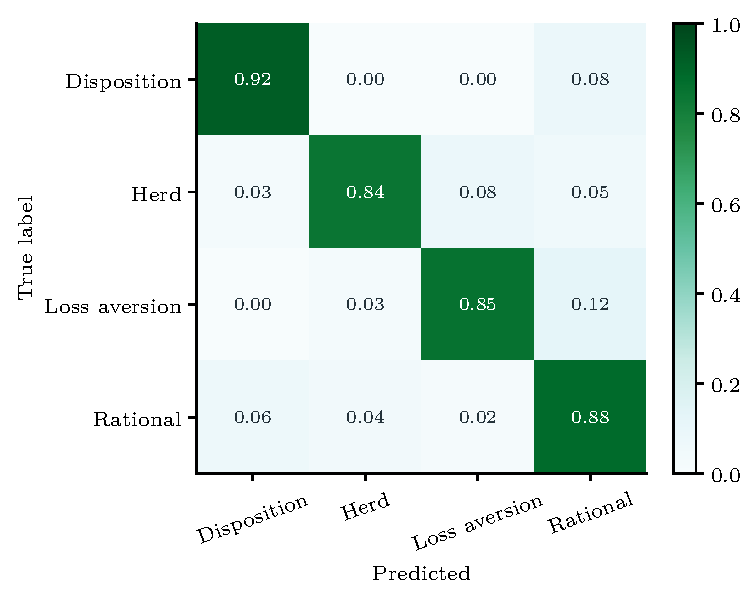
\includegraphics[width=\textwidth]{figures/charts/confusion.pdf}
\caption{Confusion matrix (rows normalized, real frequency)}
\label{fig:confusion}
\end{minipage}\hfill
\begin{minipage}[t]{0.47\textwidth}
\centering
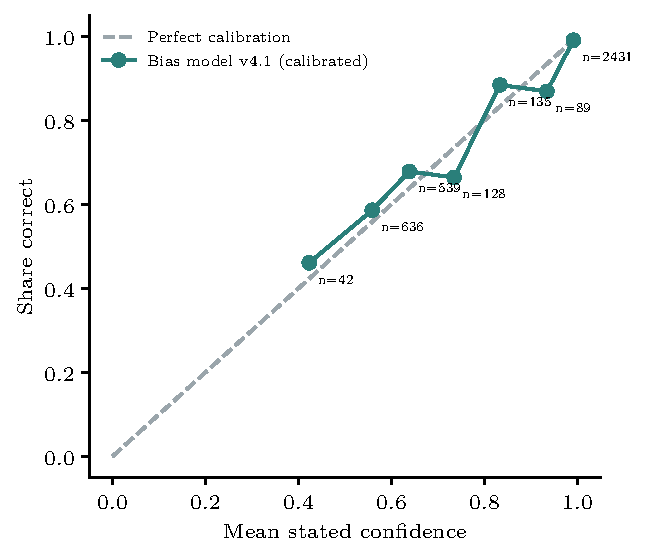
\includegraphics[width=\textwidth]{figures/charts/reliability.pdf}
\caption{Reliability diagram after calibration}
\label{fig:reliability}
\end{minipage}
\end{figure}

\begin{table}[H]
\centering
\small
\begin{tabular}{|l|c|c|c|}
\hline
\textbf{Pattern} & \textbf{Precision} & \textbf{Recall} & \textbf{F1} \\
\hline
Disposition effect & 0.844 & 0.918 & 0.879 \\
\hline
Herd behavior & 0.819 & 0.838 & 0.828 \\
\hline
Loss aversion & 0.667 & 0.849 & 0.747 \\
\hline
Rational & 0.939 & 0.875 & 0.906 \\
\hline
\end{tabular}
\caption{Per-class metrics (real frequency)}
\label{tab:perclass}
\end{table}

Table \ref{tab:overall} gives the overall result: 87.9\% accuracy, macro-F1 of 0.840 and an expected calibration error of 0.014 on the test set. The guard and the calibration step did not change any prediction on the test set. Table \ref{tab:perclass} and Figure \ref{fig:confusion} show that loss aversion is the weakest class. In a falling and fearful market, a loss-making sale is permitted under both loss aversion (panic) and herd behavior (selling into fear), and the data cannot always tell which motive won: 8.0\% of true herd cases are read as loss aversion, and 12.2\% of true loss aversion cases are read as rational. Rational decisions are recognized with the highest precision (0.939). This matters because wrongly calling a sensible decision biased is the more harmful error for a user.

\begin{table}[H]
\centering
\small
\begin{tabular}{|l|c|c|c|}
\hline
\textbf{Band shown to the user} & \textbf{Threshold} & \textbf{Share of analyses} & \textbf{Share correct} \\
\hline
High & $\geq$ 0.85 & 68.4\% & \textbf{98.7\%} \\
\hline
Medium & 0.65 to 0.85 & 7.1\% & 74.4\% \\
\hline
Low & $<$ 0.65 & 24.5\% & 61.7\% \\
\hline
\end{tabular}
\caption{Confidence bands and how often each is right}
\label{tab:bands}
\end{table}

The calibrated points in Figure \ref{fig:reliability} lie close to the diagonal. Most cases (66\% by weight) fall in the 0.95 to 1.00 bin, where the model is right 99.1\% of the time. The bands in Table \ref{tab:bands} are what the investor sees: a High reading is right about 99 times in 100, while a Low reading usually means that two patterns are close to even. In 44.3\% of cases the definitions allow only one label (holding a winner in a calm market, for example, can only be rational), which flatters the overall figures. On the remaining 55.7\%, the cases that need judgement, accuracy is 78.3\%.

Accuracy is 89.5\% in normal markets, 87.8\% in bull markets and corrections, 90.3\% in euphoria and 77.6\% in crashes, where loss aversion and herd behavior overlap the most. By action it is 84.9\% for sales, 90.0\% for holds and 89.4\% for purchases. Trained only on decisions dated 2008 to 2019 and tested on 2020 to 2026, which includes the COVID crash, the model reaches 86.5\% accuracy and 0.826 macro-F1, close to the random-split result.

\subsection{Baselines and Other Learners}
\begin{table}[H]
\centering
\small
\begin{tabular}{|l|c|c|}
\hline
\textbf{Model (real-frequency test set)} & \textbf{Accuracy} & \textbf{Macro-F1} \\
\hline
Always ``rational'' & 57.5\% & -- \\
\hline
Previous model v3 (same test cases) & 53.4\% & 0.309 \\
\hline
Definitions only (call a bias whenever one can apply) & 85.2\% & 0.825 \\
\hline
v4.1 without the \texttt{allows} inputs & 87.6\% & 0.832 \\
\hline
\textbf{v4.1} & \textbf{87.9\%} & \textbf{0.840} \\
\hline
Ceiling: v4.1 also given the hidden tendencies & 90.0\% & 0.866 \\
\hline
\end{tabular}
\caption{Baselines, ablation and ceiling}
\label{tab:baselines}
\end{table}

Table \ref{tab:baselines} is important for reading the model honestly. Because the labels come from written definitions, a rules-only baseline already reaches 85.2\%, and the model's gain over it is 2.7 points. The value of the model is in two places. It disagrees with the rules in 9.6\% of cases and is then right 64\% of the time against 36\% for the rules, because it recognizes rebalancing, a near goal, cutting a loss and a stated need for cash. It also gives calibrated confidence, which the rules cannot. The ceiling of 90.0\% shows that about one case in ten cannot be resolved from what the app observes. The previous model v3 scored 53.4\% on the same cases because it did not see the action: across 600 test cases, changing only the action changed v4.1's answer in 83.7\% of them and v3's in none.

\begin{table}[H]
\centering
\small
\resizebox{\textwidth}{!}{\begin{tabular}{|l|c|c|c|c|}
\hline
\textbf{Model} & \textbf{Accuracy (5 seeds)} & \textbf{Accuracy, seed 7 [95\% CI]} & \textbf{XGBoost minus model} & \textbf{McNemar $p$} \\
\hline
Rules only & 84.4\% $\pm$ 0.6 & 85.2\% [83.9, 86.4] & +2.7 [+1.6, +3.8] & $2.4\times10^{-7}$ \\
\hline
Logistic regression & 84.9\% $\pm$ 0.4 & 85.5\% [84.2, 86.6] & +2.4 [+1.4, +3.4] & $1.0\times10^{-5}$ \\
\hline
Random forest & 87.0\% $\pm$ 0.5 & 87.6\% [86.5, 88.7] & +0.2 [$-$0.4, +0.9] & 0.096 \\
\hline
XGBoost & 87.2\% $\pm$ 0.6 & 87.8\% [86.7, 89.0] & -- & -- \\
\hline
\end{tabular}}
\caption{Learners compared on the same features and guard (5 split seeds; bootstrap CIs and McNemar tests on seed 7)}
\label{tab:learners}
\end{table}

\begin{figure}[H]
\centering
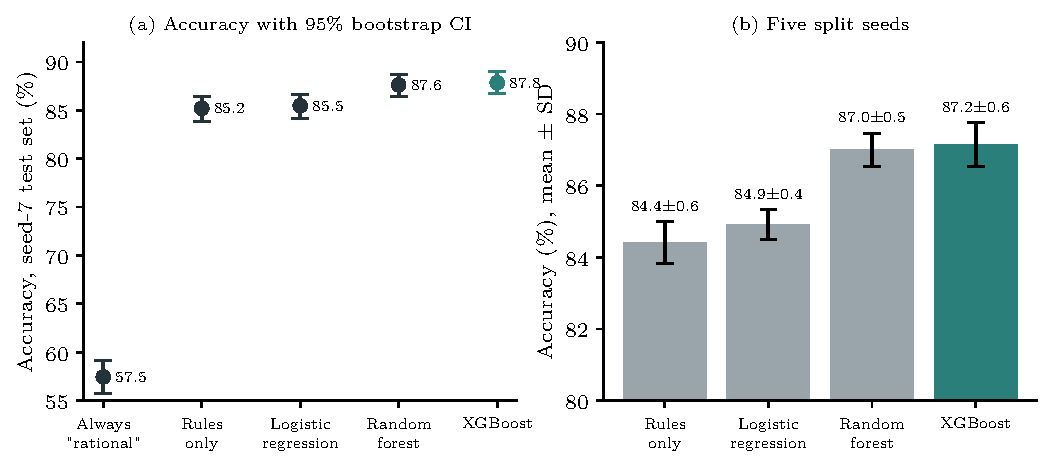
\includegraphics[width=0.95\textwidth]{figures/charts/baselines_ci.pdf}
\caption{(a) Accuracy with 95\% bootstrap confidence intervals; (b) mean and standard deviation over five split seeds}
\label{fig:learners}
\end{figure}

To check whether XGBoost is the right learner, logistic regression and a 500-tree random forest were trained on the same 22 features with the same guard and weighting, over five split seeds, with 2,000 bootstrap resamples and McNemar's test on the original split (Table \ref{tab:learners}, Figure \ref{fig:learners}). XGBoost is significantly better than the rules and logistic regression, which shows that the non-linear interactions matter. It is statistically tied with the random forest (a difference of 0.2 points with $p = 0.096$), so we do not claim that XGBoost is the better learner. It was kept because it has the lowest log-loss (0.267 against 0.282 for the forest), exact and fast TreeSHAP explanations and a portable model file.

Of the test cases, 167 are sales forced by money. Bias model v4.1 reads 71.9\% of them as rational: 90.6\% when the need is stated in the comment and 39.3\% when it is not, against 37.7\% for the earlier v4.0 model trained without money pressure. The gap between stated and unstated needs is exactly what the comment reader is designed to close. The training script also runs 13 scenario checks and 8 relational checks on a typical investor, and v4.1 passes all 21 (v3 passed 5 of the 13 scenarios). For example, selling a winner up 35\% in a calm market reads as the disposition effect with confidence 0.98, selling at a 20\% loss in a calm market reads as rational, and in a fearful market a stated cash need raises the rational reading from 0.09 to 0.49. Gold share alone barely moves the reading (largest change 0.05), as it should, since gold has no role in the label definitions.

\section{Simulator Results}
\subsection{Realism and Choice of Generator}
\begin{table}[H]
\centering
\small
\resizebox{\textwidth}{!}{\begin{tabular}{|l|c|c|c|c|c|}
\hline
\textbf{Generator} & \textbf{1-yr p10} & \textbf{1-yr median} & \textbf{1-yr p90} & \makecell{\textbf{ACF of squared}\\ \textbf{returns, lag 1/3/6}} & \textbf{KS distance} \\
\hline
Real NIFTY (217 windows) & $-$7.5\% & 11.3\% & 33.3\% & 0.136 / 0.051 / 0.093 & -- \\
\hline
Lognormal (GBM) & $-$16.2\% & 9.5\% & 42.1\% & $-$0.01 / $-$0.01 / $-$0.01 & 0.132 \\
\hline
Independent months & $-$15.9\% & 10.6\% & 41.2\% & $-$0.01 / $-$0.01 / $-$0.01 & 0.108 \\
\hline
Block 3 months & $-$14.3\% & 10.6\% & 37.8\% & 0.077 / $-$0.01 / $-$0.01 & 0.083 \\
\hline
Block 6 months & $-$13.7\% & 10.5\% & 35.9\% & 0.100 / 0.029 / $-$0.01 & 0.072 \\
\hline
\textbf{Block 12 months (used)} & \textbf{$-$8.1\%} & \textbf{10.3\%} & \textbf{33.1\%} & \textbf{0.101 / 0.035 / 0.025} & \textbf{0.027} \\
\hline
Block 24 months & $-$8.1\% & 10.3\% & 33.0\% & 0.105 / 0.023 / 0.033 & 0.030 \\
\hline
\end{tabular}}
\caption{Six market path generators against the real index (10,000 ten-year paths each, same historical mean)}
\label{tab:generators}
\end{table}

\begin{figure}[H]
\centering
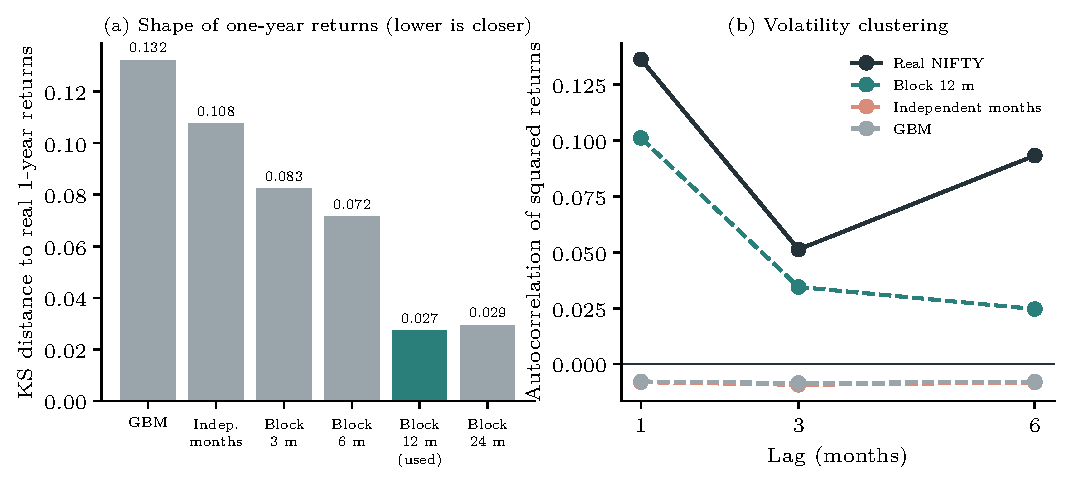
\includegraphics[width=0.95\textwidth]{figures/charts/generators.pdf}
\caption{(a) Kolmogorov-Smirnov distance to real one-year returns; (b) volatility clustering}
\label{fig:generators}
\end{figure}

Table \ref{tab:generators} and Figure \ref{fig:generators} justify the choice of generator. All six generators share the same average growth, so only the shape and the dependence differ. The 12-month block bootstrap is the only one that reproduces both the spread of real one-year returns and volatility clustering. Its KS distance (0.027) is a quarter of that of independent months (0.108) and a fifth of GBM's (0.132), while GBM and independent months have no clustering at all and make bad years about twice as bad as reality. Moving to 24-month blocks changes almost nothing. With the long-run growth assumptions used in the app, simulated one-year returns are $-$6.9\%, +11.6\% and +34.7\% at the 10th, 50th and 90th percentiles, against $-$7.5\%, +11.3\% and +33.3\% for the real index; the earlier v1 simulator had bad years of $-$15.8\%. The 19-year record holds only one independent decade, so ten-year comparisons (KS distance about 0.34 for every generator) are not used to rank generators.

\subsection{Effect of the Horizon and Stability of the Numbers}
\begin{table}[H]
\centering
\small
\begin{tabular}{|c|c|c|c|c|}
\hline
\textbf{Horizon} & \makecell{\textbf{Stock down 17\%:}\\ \textbf{holding wins}} & \textbf{Typical gap} & \makecell{\textbf{Fund up 30\%:}\\ \textbf{holding wins}} & \textbf{Typical gap} \\
\hline
1 year & 55\% & \rupee 3,592 & 66\% & \rupee 6,377 \\
\hline
3 years & 60\% & \rupee 13,950 & 70\% & \rupee 22,244 \\
\hline
5 years & 59\% & \rupee 21,124 & 70\% & \rupee 41,640 \\
\hline
10 years & 62\% & \rupee 59,925 & 75\% & \rupee 1.09 L \\
\hline
20 years & 64\% & \rupee 1.81 L & 80\% & \rupee 4.09 L \\
\hline
30 years & 61\% & \rupee 3.49 L & 81\% & \rupee 13.9 L \\
\hline
\end{tabular}
\caption{Effect of the horizon (\rupee 1 lakh position; investor earning \rupee 18 lakh a year with \rupee 11 lakh liquid)}
\label{tab:horizon}
\end{table}

\begin{figure}[H]
\centering
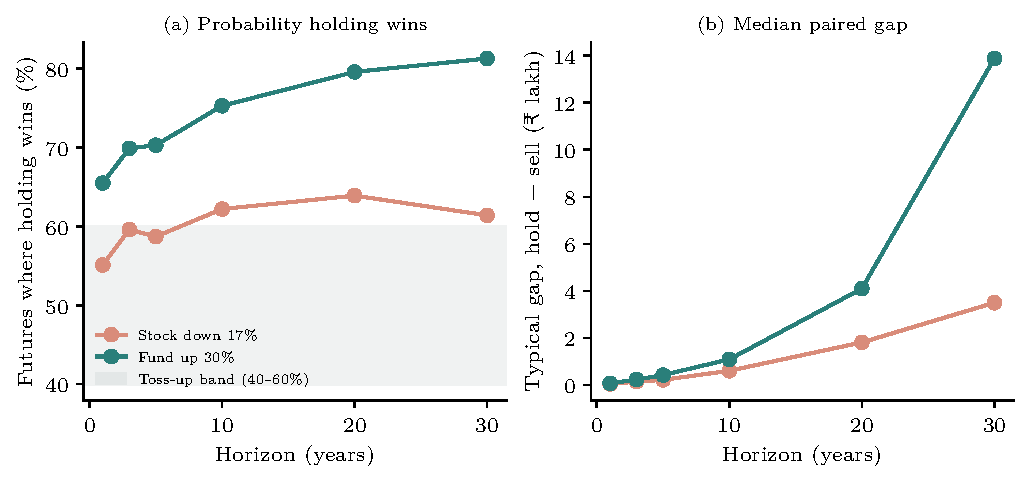
\includegraphics[width=0.95\textwidth]{figures/charts/horizon.pdf}
\caption{(a) Share of futures in which holding beats selling; (b) median paired gap, by horizon}
\label{fig:horizon}
\end{figure}

Table \ref{tab:horizon} and Figure \ref{fig:horizon} show the central practical result of the simulator. For a single stock down 17\%, the probability that holding beats selling stays between 55\% and 64\% at every horizon, mostly inside or near the band of 40 to 60\% that the recommendation rules treat as a toss-up. A diversified fund, with little company-specific risk, favors holding much more clearly and reaches 80\% at 20 years. The earlier simulator always used a 20-year horizon and therefore tilted every recommendation towards holding, even for someone who needs the money in three years.

\begin{figure}[H]
\centering
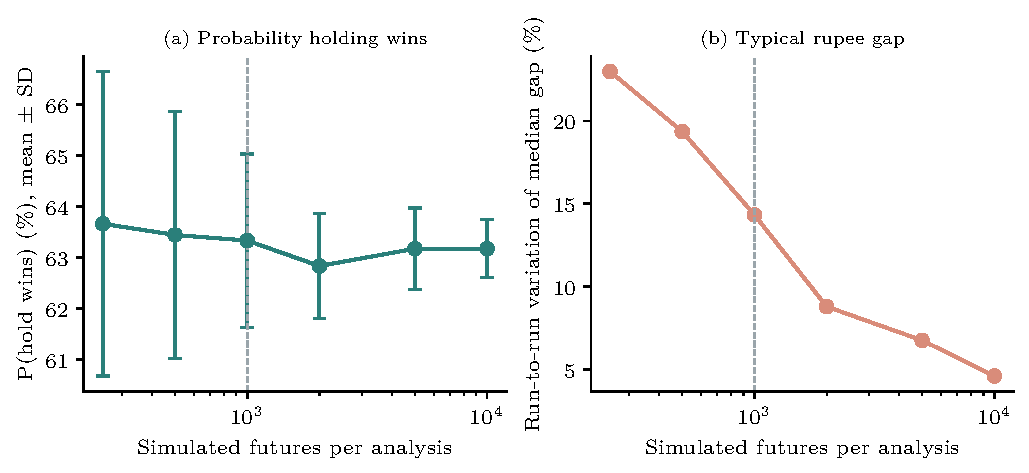
\includegraphics[width=0.95\textwidth]{figures/charts/convergence.pdf}
\caption{Monte Carlo convergence for the base case (20 repeats per size)}
\label{fig:convergence}
\end{figure}

Figure \ref{fig:convergence} shows how much of each number is simulation noise. At the app's 1,000 futures, the probability that holding wins (the input to the recommendation rules) varies by about $\pm$1.7 points between runs, close to the binomial standard error of $\pm$1.5 points. The median rupee gap is noisier and varies by about $\pm$14\%. This is why the verdict is driven by the probability and the rupee gap is presented as an approximate value.

\subsection{Results over 1,000 Investors and Sensitivity}
\begin{table}[H]
\centering
\small
\resizebox{\textwidth}{!}{\begin{tabular}{|l|c|c|c|}
\hline
\textbf{Group} & \textbf{Investors} & \textbf{Mean P(hold wins)} & \textbf{HOLD / toss-up / SELL} \\
\hline
All (long-run assumptions) & 1,000 & 0.635 & 58.1\% / 40.8\% / 1.1\% \\
\hline
Horizon 1 to 3 years & 52 & 0.571 & 29\% / 71\% / 0\% \\
\hline
Horizon 4 to 10 years & 100 & 0.598 & 43\% / 57\% / 0\% \\
\hline
Horizon 11 to 20 years & 275 & 0.624 & 57\% / 41\% / 2\% \\
\hline
Horizon 21 to 30 years & 573 & 0.652 & 64\% / 35\% / 1\% \\
\hline
Single stock & 596 & 0.562 & 31\% / 67\% / 2\% \\
\hline
Equity fund & 404 & 0.742 & 99\% / 1\% / 0\% \\
\hline
History replayed exactly & 1,000 & 0.380 & 5.6\% / 37.8\% / 56.6\% \\
\hline
\end{tabular}}
\caption{Paired simulation over 1,000 investors drawn from dataset v4.1}
\label{tab:population}
\end{table}

\begin{figure}[H]
\centering
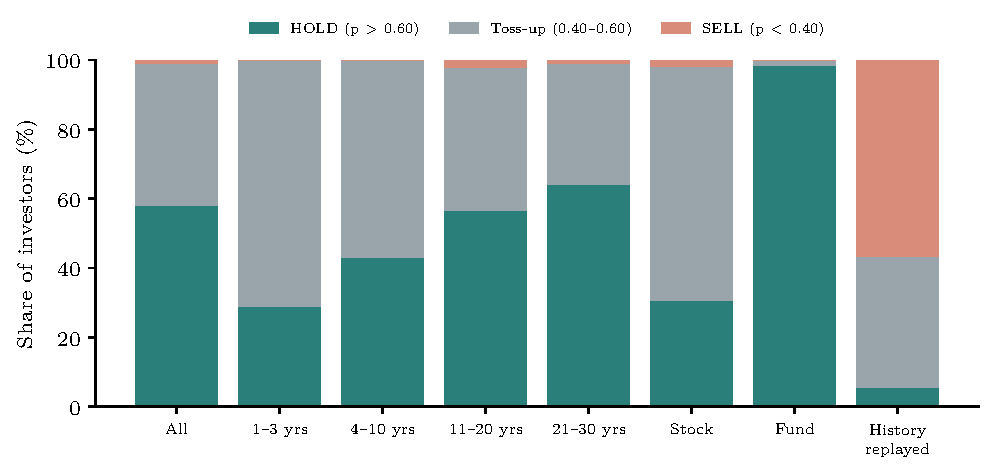
\includegraphics[width=0.9\textwidth]{figures/charts/population.pdf}
\caption{Share of investors in each verdict band}
\label{fig:population}
\end{figure}

Table \ref{tab:population} and Figure \ref{fig:population} move from single examples to a population. Under the long-run assumptions, holding is clearly favored for 58\% of investors, the comparison is a toss-up for 41\% and selling is favored for 1\%. Almost every equity fund (99\%) clearly favors holding, while only 31\% of single stocks do, because company-specific risk lowers the typical outcome. Whether the position is currently at a gain or a loss makes no difference (59\% and 57\% HOLD), which is exactly the point of the disposition effect literature: the purchase price should not matter for a forward-looking decision. The last row is the most important caution. If 2007 to 2026 is replayed exactly, gold compounds at about 15\% a year instead of 9\%, and 86\% of verdicts change.

\begin{figure}[H]
\centering
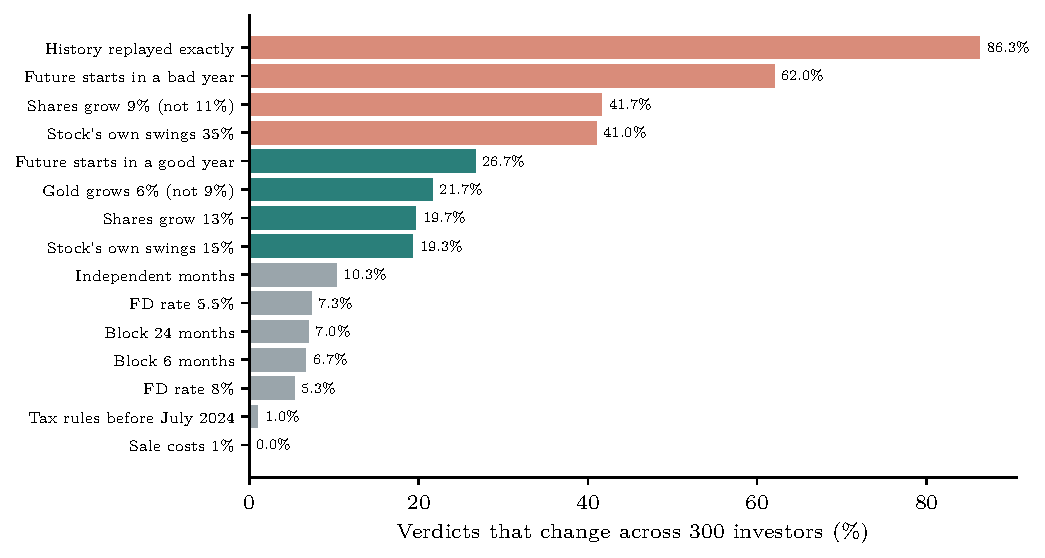
\includegraphics[width=0.85\textwidth]{figures/charts/sensitivity.pdf}
\caption{Share of verdicts that change across 300 investors when one assumption is changed}
\label{fig:sensitivity}
\end{figure}

Figure \ref{fig:sensitivity} ranks the assumptions by how many verdicts they change. The answer depends most on the growth assumptions for shares and gold (shares growing at 9\% instead of 11\% changes 41.7\% of verdicts), on how volatile the particular stock is (own volatility of 35\% instead of 21\% changes 41.0\%) and on the kind of year the future starts in (a bad first year changes 62.0\%). It barely depends on the block length, the July 2024 tax change (1.0\%) or sale costs (0\%, since the cost is charged on cashing out in both futures). This is why Folium measures each stock's risk at submission instead of assuming it, and why the growth assumptions are stated on every result page.

\begin{figure}[H]
\centering
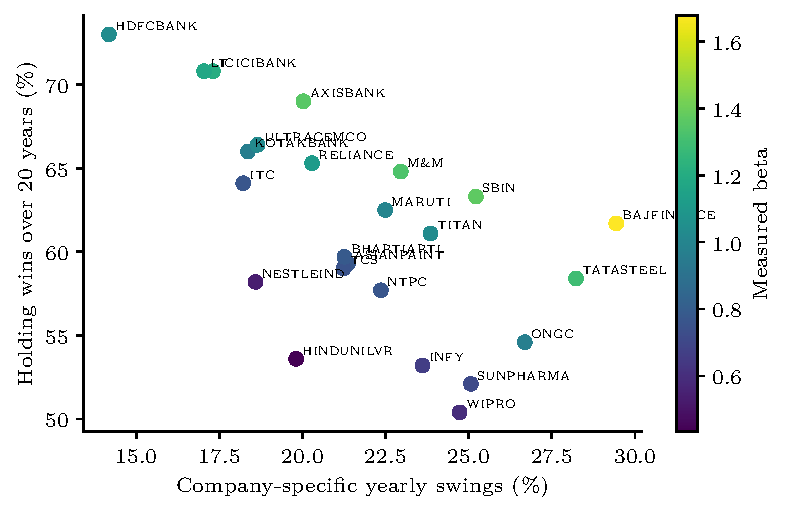
\includegraphics[width=0.75\textwidth]{figures/charts/stocks.pdf}
\caption{Company-specific volatility against the share of 20-year futures in which holding wins, for 24 NIFTY 50 stocks}
\label{fig:stocks}
\end{figure}

Figure \ref{fig:stocks} shows a clear negative relationship between a stock's own volatility and the advantage of holding it. HDFC Bank, with beta 1.03 and own volatility of 14\%, wins in 73\% of 20-year futures, while Wipro, with beta 0.60 and own volatility of 25\%, wins in 50\%. Two effects combine: own volatility drags down the median compound outcome, and a low beta lowers expected growth under the capital asset pricing relation. The second effect is a modeling choice, since steady low-beta stocks have often done better historically than the relation predicts.

\subsection{Comparison with Real History}
\begin{table}[H]
\centering
\small
\resizebox{\textwidth}{!}{\begin{tabular}{|c|c|c|c|c|c|}
\hline
\textbf{Window} & \makecell{\textbf{Real windows}\\ \textbf{(independent)}} & \makecell{\textbf{Hold won,}\\ \textbf{real}} & \makecell{\textbf{Hold won,}\\ \textbf{simulated}} & \makecell{\textbf{Real median}\\ \textbf{gap}} & \makecell{\textbf{Real inside simulated}\\ \textbf{10--90\% band}} \\
\hline
5 years & 169 (3) & 88.8\% & 61.0\% & \rupee 56,378 & 99.4\% \\
\hline
10 years & 109 (1) & 100\% & 60.7\% & \rupee 1,25,114 & 100\% \\
\hline
\end{tabular}}
\caption{Walk-forward replay of a fund up 30\% through every real window}
\label{tab:walk}
\end{table}

Table \ref{tab:walk} places what actually happened in each real 5-year and 10-year window inside the simulated distribution for the same case. Every real outcome but one falls inside the simulated 10th to 90th percentile band, and real outcomes sit in the upper middle of the band, since 2007 to 2026 was a good period for holding equity. With only one to three independent windows this is a consistency check and not a validation of forecasting ability. A related check concerns the paired gap itself: for the base-case investor over 14 years, the difference of the two medians and the median of the paired differences differ by up to 19\% at year 10 (\rupee 63,790 against \rupee 51,717). Folium reports the paired gap with its 10th to 90th percentile range ($-$\rupee 1,19,371 to \rupee 5,12,349 at year 10), because that range also shows that holding loses in a substantial share of futures even when it wins in the typical one.

\section{Cause and Effect Results}
\begin{table}[H]
\centering
\small
\resizebox{\textwidth}{!}{\begin{tabular}{|l|l|c|c|c|}
\hline
\textbf{Factor} & \textbf{Change} & \textbf{Sell} & \textbf{Hold} & \textbf{Buy more} \\
\hline
A cash shock & having one vs not & +31.8 (+31.3) & $-$23.6 ($-$23.3) & $-$8.2 ($-$8.0) \\
\hline
Emergency fund & having one vs not & $-$7.5 ($-$5.6) & +1.4 ($-$0.1) & +6.1 (+5.7) \\
\hline
Market fear & VIX +10 points & +6.4 (+3.9) & $-$4.7 ($-$2.9) & $-$1.7 ($-$1.0) \\
\hline
Weaker NIFTY month & 5 points worse & +5.6 (+5.8) & $-$3.9 ($-$3.7) & $-$1.7 ($-$2.1) \\
\hline
Bigger holding & +10 points of liquid & +4.8 (+4.7) & +2.7 (+2.8) & $-$7.5 ($-$7.5) \\
\hline
Longer horizon & +5 years & $-$2.4 ($-$2.3) & +1.4 (+1.4) & +1.0 (+1.0) \\
\hline
Gold (negative control) & +10 points & 0.0 ($-$0.2) & 0.0 (+0.4) & 0.0 ($-$0.2) \\
\hline
\end{tabular}}
\caption{Average effects in percentage points: true value, with the g-computation estimate in brackets}
\label{tab:effects}
\end{table}

\begin{figure}[H]
\centering
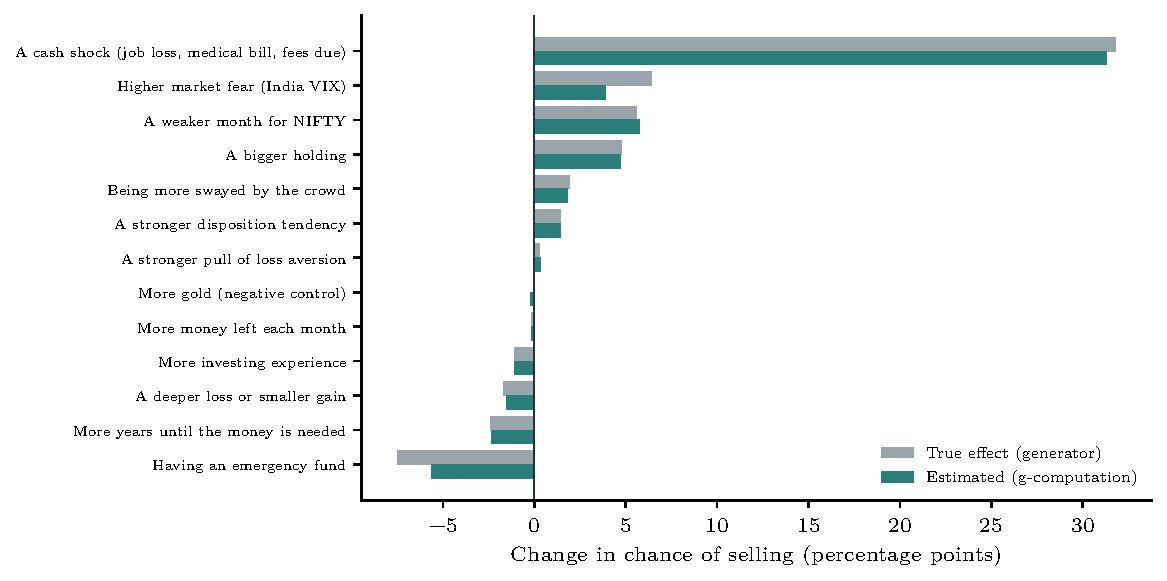
\includegraphics[width=0.92\textwidth]{figures/charts/causal.pdf}
\caption{Effect of each factor on the chance of selling: true effect against the g-computation estimate}
\label{fig:causal}
\end{figure}

Table \ref{tab:effects} and Figure \ref{fig:causal} show that money pressure dominates. A cash shock raises the chance of selling by about 32 points, and an emergency fund lowers it by 7.5 points, mostly by absorbing shocks. Market fear and a weak month push towards selling, and a bigger holding pushes towards selling (largely through rebalancing) and strongly away from adding. Loss aversion's population-wide effect is small (+0.3 points) because it acts only in specific situations; within them it is large.

Across all 45 effects, the g-computation estimates have a mean absolute error of 0.48 points and the correct direction in 97\% of cases. For effects on selling, g-computation's error is 0.45 points against 1.07 for the linear DoWhy model, which for example overstates the effect of investing experience about fivefold. The linear model is better at the effect of a tendency within its own situation (0.3 points against 1.4). DoWhy passed 12 of 13 refutation tests; the one failure is the gold negative control, whose true effect is zero, so a test against chance cannot confirm anything. When the most helpful habit is applied in each situation, the estimates always move in the right direction and, where they are off, they understate the benefit. For example, setting selling rules in advance lowers the share of winners sold in a calm market from 56\% to 39\% in truth, and the estimate gives 54\% to 40\%. One unexpected finding is that habits can work against each other: for someone holding a deep loser, all three habits together barely help (43\% to 42\%), while reframing the loss alone helps a lot (43\% to 36\%). For this reason the app offers the single most helpful habit and never a bundle.

\section{Explanation Quality}
Explanation quality was measured on the current pipeline for 166 sell and hold decisions drawn from the population study, explained in both English and Hindi (332 explanations), with AI wording switched off. Every explanation was complete (all six sections present), actionable and personalized, and none contained a jargon term. The English explanations have a mean Flesch reading ease of 76.4 (minimum 73.5, against a target of 60), which corresponds to fairly easy text, with 11.3 words per sentence. The Hindi explanations average 12.8 words per sentence against a target of 20; Flesch is not used for Hindi because its syllable model is undefined for Devanagari. These are measures of structure and readability; they do not show that the explanations change investor behavior, which would need a user study.

\section{Application Screenshots}
The screenshots in this section are to be captured from the running application with the demonstration accounts created by \texttt{scripts/seed\_demo.py}.

\newcommand{\screenshot}[2]{%
\begin{figure}[H]
\centering
\fbox{\parbox[c][5.2cm][c]{0.8\textwidth}{\centering\textit{Screenshot to be inserted}\\[4pt]#1}}
\caption{#2}
\end{figure}}
\screenshot{Result page}{Result page with the recommendation, both futures and the pattern found}
\screenshot{Live progress}{Live five-step progress during an analysis}
\screenshot{Hindi explanation}{Six-part explanation in Hindi}
\screenshot{Portfolio page}{Portfolio page with net worth, allocation and holdings}
\screenshot{Verify this record}{Verification of an audit record}
\screenshot{Google sign-in and Welcome page}{Google sign-in return and the Welcome profile step}

\section{Discussion}
On the development task, each analytical component does what it was designed to do. The classifier is accurate, calibrated and consistent with the label definitions, significantly better than the rules and a linear model and on par with a random forest. It changes its reading when the action changes, recognizes forced sales when the need is stated and generalizes across time periods within the data. The simulator's generator was chosen experimentally against five alternatives. It reproduces the real index's one-year distribution and volatility clustering, its probability output is stable at the app's path count, and every real window falls inside its band. The causal estimates recover a known mechanism closely and never overclaim the benefit of habits, and the explanations are complete, readable and free of jargon on the current models.

The results also have clear boundaries. The behavioral labels are synthetic, so 87.9\% accuracy means that the model recovers the generator's labels, not that it diagnoses real investors, and most of that accuracy follows from the definitions themselves. The simulator's agreement with history is a distributional check and not a forecast, and its verdicts depend heavily on the stated growth assumptions. The causal results describe the generator and not people, and no study has measured whether investors who use Folium decide differently.

The combination is more useful than any part alone. For a typical request to sell a falling stock, the simulator often lands in the toss-up band (two-thirds of single-stock positions do), and the behavioral reading then decides whether waiting is the cautious choice. A stated need for cash moves the reading to rational and lets the sale stand. The investor sees why, in their own language, with every figure traceable, and can later check that the record has not been changed.

\chapter{Testing}
Testing in Folium had four goals: to show that each model and engine behaves as specified, including behavioral properties and not only code paths; to show that the security controls block what they are meant to block; to show that the pipeline, database and live stream work together; and to prevent regressions when models are retrained or replaced.

\section{Test Suites}
\begin{table}[H]
\centering
\small
\begin{tabularx}{\textwidth}{|P{3.2cm}|P{3.9cm}|c|L|}
\hline
\textbf{Suite} & \textbf{Location} & \textbf{Tests} & \textbf{Needs} \\
\hline
Models and engines & \texttt{tests/} & 343 & Python environment (5 tests need an AI key) \\
\hline
Back end, full & \texttt{backend/tests/} & 267 & PostgreSQL and Redis (149 of these run without a database) \\
\hline
Front end & \texttt{frontend/src/test/} & 25 & Node.js (Vitest, Testing Library) \\
\hline
\end{tabularx}
\caption{Automated test suites (635 tests in total)}
\label{tab:suites}
\end{table}

The counts in Table \ref{tab:suites} are those recorded in the project's master reference after the latest changes, where all suites were reported as passing. Many tests are parameterized, so one test function runs over several cases.

\section{Unit Testing}
\begin{table}[H]
\centering
\small
\begin{tabularx}{\textwidth}{|c|P{5.6cm}|L|}
\hline
\textbf{ID} & \textbf{Test} & \textbf{Property checked} \\
\hline
UT-1 & Training and live features agree & One row and a batch build identical features \\
\hline
UT-2 & Invalid input rejected & A missing input or unknown action raises an error \\
\hline
UT-3 & Label rules match the dataset & The true label is allowed for all 20,000 rows \\
\hline
UT-4 & Guard and calibration & Ruled-out classes are removed; calibration never changes the chosen class \\
\hline
UT-5 & SHAP drivers & Drivers sum to the chosen class's score \\
\hline
UT-6 & Action sensitivity & The same situation with a different action gives a different reading \\
\hline
UT-7 & Tax rules & 20\% short-term tax with cess; \rupee 1.25 lakh exemption; losses pay nothing \\
\hline
UT-8 & Simulator behavior & Horizon clamped to 1 to 30 years; same inputs give the same answer; SIP leaves the gap unchanged; simulated years resemble the real NIFTY \\
\hline
UT-9 & Recommendation rules & Every combination of intent, pattern and $p$; a missing simulation is disclosed \\
\hline
UT-10 & Audit chain & An edited, removed or forged entry and a fork are all caught; fingerprints survive database round trips \\
\hline
UT-11 & Comment reading & Rules in three languages; quotes are verbatim; both-sides cases never alter the verdict \\
\hline
UT-12 & Explanations & Six sections, English and Hindi structural parity, jargon blocklist, number check \\
\hline
\end{tabularx}
\caption{Representative unit tests}
\label{tab:unit}
\end{table}

\section{Integration Testing}
Integration tests run the FastAPI application against real PostgreSQL and Redis instances through an HTTP client.

\begin{table}[H]
\centering
\small
\begin{tabularx}{\textwidth}{|c|P{5cm}|L|}
\hline
\textbf{ID} & \textbf{Scenario} & \textbf{Expected result} \\
\hline
IT-1 & Register, verify, log in, refresh, log out & Cookies set and rotated; old tokens blacklisted \\
\hline
IT-2 & Enable TOTP; log in with a code and a backup code & Second factor enforced; backup code single-use \\
\hline
IT-3 & Mutating request with missing, wrong and correct CSRF header & 403, 403, accepted; login exempt \\
\hline
IT-4 & User B queries user A's rows; query with no user set & No rows in either case \\
\hline
IT-5 & Repeated logins beyond the limit & HTTP 429 \\
\hline
IT-6 & Submit an analysis and run the pipeline & 202; status moves to processing and then complete \\
\hline
IT-7 & Open the stream during and after a run & Backlog replayed without duplicates; final event received \\
\hline
IT-8 & Two analyses, then tamper with a row and verify & Chain stays linear; the changed part is named \\
\hline
IT-9 & Reason says ``college fees are due'' & Cash need detected; sale can read as rational \\
\hline
IT-10 & Delete, log in during grace, purge after grace & ``Keep my account'' offered; data anonymized; audit kept \\
\hline
IT-11 & Google sign-in with a stand-in for Google & Correct redirect for each outcome; unverified addresses refused; state single-use \\
\hline
IT-12 & Google return page for each outcome (front end) & Signs in, asks for the code, offers to keep the account or explains the failure \\
\hline
\end{tabularx}
\caption{Integration test scenarios}
\label{tab:integration}
\end{table}

\section{System Testing}
The behavior of the product as a whole is exercised through the demonstration walkthrough, which uses accounts and analyses created by the seeding script. Table \ref{tab:system} lists the system test cases with their expected results.

\begin{table}[H]
\centering
\small
\begin{tabularx}{\textwidth}{|c|P{5.4cm}|L|}
\hline
\textbf{ID} & \textbf{Test case} & \textbf{Expected result} \\
\hline
ST-1 & Sell a losing holding with the reason ``need money for college fees in March'' & Pattern reads rational and the quote is shown \\
\hline
ST-2 & Sell a holding up 30\% in a calm market & Disposition effect with High or Medium confidence \\
\hline
ST-3 & Buy more after a NIFTY rise of 5\% in a month & Herd reading and a HOLD verdict \\
\hline
ST-4 & Switch the explanation to Hindi & All six sections in Hindi with the same numbers \\
\hline
ST-5 & Request a Hindi PDF report & Refused with an explanation; HTML offered \\
\hline
ST-6 & Reload the page during step 2 & Earlier steps shown from the backlog; progress continues \\
\hline
ST-7 & Verify a record, then edit it in the database and verify again & ``Verified'', then ``Changed'' with the changed part named \\
\hline
ST-8 & Run an analysis with market data switched off & Calm market assumed and disclosed \\
\hline
ST-9 & First sign-in with a new Google account & Returns to the app; Welcome page asks for the profile \\
\hline
\end{tabularx}
\caption{System test cases}
\label{tab:system}
\end{table}

\section{Validation, Edge Cases and Performance}
Input is validated at three layers. Pydantic schemas reject malformed requests with HTTP 422 before any logic runs. Database check constraints enforce domain rules whatever the code path, for example that age lies between 18 and 100, that the quantity is positive, that confidence lies between 0 and 1, and that a recommendation is one of HOLD, SELL or BUY MORE. The model and the simulator raise an error on missing or invalid inputs. The edge cases of Table \ref{tab:edge} are covered by tests such as horizon clamping, the missing-simulation rule and the price outage.

No load test has been performed. One simulation of 1,000 paths over 30 years takes 103.4 ms, and each prediction records its own inference time in milliseconds. Numerical stability, which matters more for the correctness of a verdict, was measured instead: at 1,000 paths the probability that holding wins varies by only about $\pm$1.7 points between runs.

\section{Defects Found and Resolved}
\begin{table}[H]
\centering
\small
\begin{tabularx}{\textwidth}{|c|L|P{4.4cm}|}
\hline
\textbf{\#} & \textbf{Issue} & \textbf{Status} \\
\hline
1 & The application connected as a superuser, which bypasses row-level security & Fixed: connects as \texttt{app\_user} \\
\hline
2 & v3's explanation described a different class from the one shown (98.6\% of cases) & Fixed in v4 \\
\hline
3 & The Google sign-in callback returned JSON instead of returning to the app & Fixed: redirect and Welcome page \\
\hline
4 & The slab rate on interest was computed from take-home pay & Fixed: income grossed up \\
\hline
5 & A driver label read ``Your choice to holding on'' & Fixed: separate verb mapping \\
\hline
6 & The fallback story always said ``over 20 years'' & Fixed: uses the actual horizon \\
\hline
7 & The explanation evaluation had been run on earlier models & Fixed: re-measured on 332 explanations \\
\hline
8 & The AI wording check rejects added numbers but not removed ones & Open \\
\hline
9 & Some column names still end in \texttt{\_20y} although the horizon is variable & Open (cosmetic) \\
\hline
\end{tabularx}
\caption{Defects and their status}
\label{tab:defects}
\end{table}

\chapter{Conclusion and Future Scope}
\section{Conclusion}
Retail investors often decide to sell, hold or buy more under the pull of recent losses, market fear or the crowd, while the tools available to them describe the asset rather than the decision. In this project we built Folium, a full-stack web application that judges one intended decision against the investor's whole financial picture. For each decision, a five-step background pipeline reads the investor's comment, classifies the behavioral pattern with a calibrated and guarded XGBoost model explained by exact TreeSHAP, projects holding and selling on the same block-bootstrapped market paths after Indian tax, attaches causal estimates validated against a known generator, renders a six-part explanation in English and Hindi, derives a verdict from explicit evidence rules, and seals the analysis in a per-investor hash chain. Investors sign in by e-mail or with Google, accounts are protected with two-step verification, CSRF protection and rate limits, and investors can export or delete their data.

\begin{table}[H]
\centering
\small
\begin{tabularx}{\textwidth}{|P{3.8cm}|L|}
\hline
\textbf{Objective} & \textbf{Outcome} \\
\hline
Causal decision-time framework for detecting behavioral biases & 87.9\% accuracy, macro-F1 0.840 and ECE 0.014; High readings right 98.7\% of the time; 21 of 21 sense checks; 86.5\% on an unseen period; 45 causal effects recovered with 0.48 points mean error and the correct direction in 97\% of cases \\
\hline
Personalized portfolio-level long-horizon simulation & Horizon of 1 to 30 years, after tax, on paired paths; one-year returns within 1.4 points of the real NIFTY; best of six generators (KS 0.027); probability stable to $\pm$1.7 points at 1,000 paths \\
\hline
Decision-centric counterfactual explanations & Six-part explanations in English and Hindi with year-by-year projections of both choices; 332 explanations complete and jargon-free; English Flesch reading ease 76.4 \\
\hline
Tamper-proof audit mechanism & SHA-256 hash chain for every analysis with verification that detects altered, removed and forged entries and forks; append-only table; per-investor locking \\
\hline
\end{tabularx}
\caption{Achievement of the objectives}
\label{tab:achieved}
\end{table}

Table \ref{tab:achieved} summarizes how each objective was met. All figures are development-stage results on synthetic behavioral labels.

\section{Limitations}
\label{sec:boundaries}
Two boundaries define what the results can claim. The first is scientific. The behavioral labels are synthetic by design, because no public dataset links Indian investors' decisions to their finances and true motives. The readings are therefore validated against a known generator and not against real people, and no claim is made that the system improves investment outcomes. The second concerns modeling. The simulator's verdicts depend on stated long-run growth rates, projections are in nominal rupees, tax handling is simplified (losses are not set off against other gains), mutual funds are treated as equity funds, and each analysis concerns one position. Both boundaries are stated to the investor on every result page.

\section{Future Scope}
The remaining work is organized in three phases, each building on foundations that already exist in the repository.

\begin{table}[H]
\centering
\small
\begin{tabularx}{\textwidth}{|P{2.9cm}|P{3.9cm}|L|}
\hline
\textbf{Phase} & \textbf{Milestone} & \textbf{Foundation already in place} \\
\hline
\multirow{4}{2.9cm}{Productization} & Administrator console (usage statistics, user management, recovery queue) & Aggregate statistics view without personal data; audited two-step reset endpoints; admin role \\
\cline{2-3}
 & Continuous integration & 635 tests that run with one command per suite; pinned dependencies \\
\cline{2-3}
 & Public deployment with HTTPS and production e-mail & Container definitions; secure cookies and CORS outside development; e-mail integration \\
\cline{2-3}
 & Live AI assistance & Consent switch, verbatim-quote and number checks, circuit breaker, all tested with a stand-in \\
\hline
\multirow{3}{2.9cm}{Validation with real users} & Consented real decisions, so that motive weights can be learned & Data export and consent model; outcome-tracking columns in the decisions table \\
\cline{2-3}
 & Prospective user study & Explanation engine with measured readability \\
\cline{2-3}
 & Two-way number check for AI wording & Existing check and its tests \\
\hline
\multirow{3}{2.9cm}{Richer analysis} & Inflation-adjusted output, debt and hybrid funds, loss set-off, other uses of sale proceeds & Evaluation hooks in the simulator; sensitivity framework \\
\cline{2-3}
 & Whole-portfolio decisions & Portfolio snapshot and asset-mix computation \\
\cline{2-3}
 & More Indian languages; background job queue and load testing & Bilingual template banks with parity tests; stateless API with shared state in Redis \\
\hline
\end{tabularx}
\caption{Future scope by phase}
\label{tab:roadmap}
\end{table}

The first phase turns a complete local product into a public service, the second turns development-stage evidence into evidence about people, and the third widens what the system can analyze. Longer-term ideas from the original plan, such as broker integration, alerts and periodic retraining from tracked outcomes, follow naturally once real outcome data is available. Until then, Folium should be presented exactly as it presents itself: as information and education, and not as investment advice.

\begin{thebibliography}{99}
\raggedright
\addcontentsline{toc}{chapter}{Bibliography}
\bibitem{b1} D. Kahneman and A. Tversky, ``Prospect theory: An analysis of decision under risk,'' \textit{Econometrica}, vol. 47, no. 2, pp. 263--291, 1979, doi: 10.2307/1914185.
\bibitem{b2} T. Odean, ``Are investors reluctant to realize their losses?'' \textit{The Journal of Finance}, vol. 53, no. 5, pp. 1775--1798, 1998, doi: 10.1111/0022-1082.00072.
\bibitem{b3} S. Bikhchandani, D. Hirshleifer and I. Welch, ``A theory of fads, fashion, custom, and cultural change as informational cascades,'' \textit{Journal of Political Economy}, vol. 100, no. 5, pp. 992--1026, 1992, doi: 10.1086/261849.
\bibitem{b4} H. Shefrin and M. Statman, ``The disposition to sell winners too early and ride losers too long: Theory and evidence,'' \textit{The Journal of Finance}, vol. 40, no. 3, pp. 777--790, 1985, doi: 10.1111/j.1540-6261.1985.tb05002.x.
\bibitem{b5} T. Chen and C. Guestrin, ``XGBoost: A scalable tree boosting system,'' in \textit{Proc. 22nd ACM SIGKDD Int. Conf. Knowledge Discovery and Data Mining}, 2016, pp. 785--794, doi: 10.1145/2939672.2939785.
\bibitem{b6} B. Zadrozny and C. Elkan, ``Transforming classifier scores into accurate multiclass probability estimates,'' in \textit{Proc. 8th ACM SIGKDD Int. Conf. Knowledge Discovery and Data Mining}, 2002, pp. 694--699, doi: 10.1145/775047.775151.
\bibitem{b7} S. M. Lundberg and S.-I. Lee, ``A unified approach to interpreting model predictions,'' in \textit{Advances in Neural Information Processing Systems}, vol. 30, 2017, pp. 4765--4774.
\bibitem{b8} M. T. Ribeiro, S. Singh and C. Guestrin, ``Why should I trust you?: Explaining the predictions of any classifier,'' in \textit{Proc. 22nd ACM SIGKDD}, 2016, pp. 1135--1144, doi: 10.1145/2939672.2939778.
\bibitem{b9} S. Wachter, B. Mittelstadt and C. Russell, ``Counterfactual explanations without opening the black box: Automated decisions and the GDPR,'' \textit{Harvard Journal of Law \& Technology}, vol. 31, no. 2, pp. 841--887, 2018.
\bibitem{b10} J. Pearl, \textit{Causality: Models, Reasoning, and Inference}, 2nd ed. Cambridge, U.K.: Cambridge University Press, 2009.
\bibitem{b11} A. Sharma and E. Kiciman, ``DoWhy: An end-to-end library for causal inference,'' arXiv:2011.04216, 2020.
\bibitem{b12} H. R. Künsch, ``The jackknife and the bootstrap for general stationary observations,'' \textit{The Annals of Statistics}, vol. 17, no. 3, pp. 1217--1241, 1989, doi: 10.1214/aos/1176347265.
\bibitem{b13} B. Efron and R. J. Tibshirani, \textit{An Introduction to the Bootstrap}. New York, NY, USA: Chapman \& Hall, 1993.
\bibitem{b14} B. M. Barber and T. Odean, ``Trading is hazardous to your wealth: The common stock investment performance of individual investors,'' \textit{The Journal of Finance}, vol. 55, no. 2, pp. 773--806, 2000, doi: 10.1111/0022-1082.00226.
\bibitem{b15} B. M. Barber and T. Odean, ``Boys will be boys: Gender, overconfidence, and common stock investment,'' \textit{The Quarterly Journal of Economics}, vol. 116, no. 1, pp. 261--292, 2001, doi: 10.1162/003355301556400.
\bibitem{b16} M. Grinblatt and M. Keloharju, ``What makes investors trade?'' \textit{The Journal of Finance}, vol. 56, no. 2, pp. 589--616, 2001, doi: 10.1111/0022-1082.00338.
\bibitem{b17} A. Tversky and D. Kahneman, ``Advances in prospect theory: Cumulative representation of uncertainty,'' \textit{Journal of Risk and Uncertainty}, vol. 5, pp. 297--323, 1992, doi: 10.1007/BF00122574.
\bibitem{b18} R. Thaler, ``Mental accounting and consumer choice,'' \textit{Marketing Science}, vol. 4, no. 3, pp. 199--214, 1985, doi: 10.1287/mksc.4.3.199.
\bibitem{b19} J. B. De Long, A. Shleifer, L. H. Summers and R. J. Waldmann, ``Noise trader risk in financial markets,'' \textit{Journal of Political Economy}, vol. 98, no. 4, pp. 703--738, 1990, doi: 10.1086/261703.
\bibitem{b20} E. F. Fama, ``Efficient capital markets: A review of theory and empirical work,'' \textit{The Journal of Finance}, vol. 25, no. 2, pp. 383--417, 1970, doi: 10.2307/2325486.
\bibitem{b21} H. Markowitz, ``Portfolio selection,'' \textit{The Journal of Finance}, vol. 7, no. 1, pp. 77--91, 1952, doi: 10.2307/2975974.
\bibitem{b22} R. C. Merton, ``Lifetime portfolio selection under uncertainty: The continuous-time case,'' \textit{The Review of Economics and Statistics}, vol. 51, no. 3, pp. 247--257, 1969, doi: 10.2307/1926560.
\bibitem{b23} J. D. Hamilton, ``A new approach to the economic analysis of nonstationary time series and the business cycle,'' \textit{Econometrica}, vol. 57, no. 2, pp. 357--384, 1989, doi: 10.2307/1912559.
\bibitem{b24} M. López de Prado, \textit{Advances in Financial Machine Learning}. Hoboken, NJ, USA: Wiley, 2018.
\bibitem{b25} L. Breiman, ``Random forests,'' \textit{Machine Learning}, vol. 45, pp. 5--32, 2001, doi: 10.1023/A:1010933404324.
\bibitem{b26} J. H. Friedman, ``Greedy function approximation: A gradient boosting machine,'' \textit{The Annals of Statistics}, vol. 29, no. 5, pp. 1189--1232, 2001, doi: 10.1214/aos/1013203451.
\bibitem{b27} A. Niculescu-Mizil and R. Caruana, ``Predicting good probabilities with supervised learning,'' in \textit{Proc. 22nd Int. Conf. Machine Learning (ICML)}, 2005, pp. 625--632, doi: 10.1145/1102351.1102430.
\bibitem{b28} C. Guo, G. Pleiss, Y. Sun and K. Q. Weinberger, ``On calibration of modern neural networks,'' in \textit{Proc. 34th Int. Conf. Machine Learning (ICML)}, PMLR 70, 2017, pp. 1321--1330.
\bibitem{b29} T. Saito and M. Rehmsmeier, ``The precision-recall plot is more informative than the ROC plot when evaluating binary classifiers on imbalanced datasets,'' \textit{PLOS ONE}, vol. 10, no. 3, e0118432, 2015, doi: 10.1371/journal.pone.0118432.
\bibitem{b30} R. K. Mothilal, A. Sharma and C. Tan, ``Explaining machine learning classifiers through diverse counterfactual explanations,'' in \textit{Proc. Conf. Fairness, Accountability, and Transparency (FAT*)}, 2020, pp. 607--617, doi: 10.1145/3351095.3372850.
\bibitem{b31} D. Janzing, L. Minorics and P. Blöbaum, ``Feature relevance quantification in explainable AI: A causal problem,'' in \textit{Proc. 23rd Int. Conf. Artificial Intelligence and Statistics (AISTATS)}, PMLR 108, 2020, pp. 2907--2916.
\bibitem{b32} V. Chernozhukov, D. Chetverikov, M. Demirer, E. Duflo, C. Hansen, W. Newey and J. Robins, ``Double/debiased machine learning for treatment and structural parameters,'' \textit{The Econometrics Journal}, vol. 21, no. 1, pp. C1--C68, 2018, doi: 10.1111/ectj.12097.
\bibitem{b33} D. N. Politis and J. P. Romano, ``The stationary bootstrap,'' \textit{Journal of the American Statistical Association}, vol. 89, no. 428, pp. 1303--1313, 1994, doi: 10.1080/01621459.1994.10476870.
\bibitem{b34} P. Weber, K. V. Carl and O. Hinz, ``Applications of explainable artificial intelligence in finance: A systematic review of finance, information systems, and computer science literature,'' \textit{Management Review Quarterly}, vol. 74, pp. 867--907, 2024, doi: 10.1007/s11301-023-00320-0.
\bibitem{b35} S. M. Lundberg, G. Erion, H. Chen, A. DeGrave, J. M. Prutkin, B. Nair, R. Katz, J. Himmelfarb, N. Bansal and S.-I. Lee, ``From local explanations to global understanding with explainable AI for trees,'' \textit{Nature Machine Intelligence}, vol. 2, pp. 56--67, 2020, doi: 10.1038/s42256-019-0138-9.
\bibitem{b36} J. Robins, ``A new approach to causal inference in mortality studies with a sustained exposure period: Application to control of the healthy worker survivor effect,'' \textit{Mathematical Modelling}, vol. 7, no. 9--12, pp. 1393--1512, 1986, doi: 10.1016/0270-0255(86)90088-6.
\bibitem{b37} M. A. Hernán and J. M. Robins, \textit{Causal Inference: What If}. Boca Raton, FL, USA: Chapman \& Hall/CRC, 2020.
\bibitem{b38} M. Jones, J. Bradley and N. Sakimura, ``JSON Web Token (JWT),'' IETF RFC 7519, May 2015, doi: 10.17487/RFC7519.
\bibitem{b39} D. M'Raihi, S. Machani, M. Pei and J. Rydell, ``TOTP: Time-Based One-Time Password Algorithm,'' IETF RFC 6238, May 2011, doi: 10.17487/RFC6238.
\bibitem{b40} N. Provos and D. Mazières, ``A future-adaptable password scheme,'' in \textit{Proc. USENIX Annual Technical Conference (FREENIX Track)}, 1999, pp. 81--91.
\bibitem{b41} D. L. Wheeler, ``zxcvbn: Low-budget password strength estimation,'' in \textit{Proc. 25th USENIX Security Symposium}, 2016, pp. 157--173.
\bibitem{b42} OWASP Foundation, ``Cross-Site Request Forgery Prevention Cheat Sheet,'' OWASP Cheat Sheet Series. [Online]. Available: \url{https://cheatsheetseries.owasp.org/cheatsheets/Cross-Site_Request_Forgery_Prevention_Cheat_Sheet.html}
\bibitem{b43} The PostgreSQL Global Development Group, ``Row Security Policies,'' \textit{PostgreSQL Documentation}. [Online]. Available: \url{https://www.postgresql.org/docs/current/ddl-rowsecurity.html}
\bibitem{b44} S. Haber and W. S. Stornetta, ``How to time-stamp a digital document,'' \textit{Journal of Cryptology}, vol. 3, no. 2, pp. 99--111, 1991, doi: 10.1007/BF00196791.
\bibitem{b45} National Institute of Standards and Technology, ``Secure Hash Standard (SHS),'' FIPS PUB 180-4, Aug. 2015, doi: 10.6028/NIST.FIPS.180-4.
\bibitem{b46} WHATWG, ``Server-sent events,'' \textit{HTML Living Standard}. [Online]. Available: \url{https://html.spec.whatwg.org/multipage/server-sent-events.html}
\bibitem{b47} A. P. Oron and N. Flournoy, ``Centered isotonic regression: Point and interval estimation for dose-response studies,'' \textit{Statistics in Biopharmaceutical Research}, vol. 9, no. 3, pp. 258--267, 2017, doi: 10.1080/19466315.2017.1286256.
\bibitem{b48} F. Pedregosa \textit{et al.}, ``Scikit-learn: Machine learning in Python,'' \textit{Journal of Machine Learning Research}, vol. 12, pp. 2825--2830, 2011.
\bibitem{b52} R. Aroussi, ``yfinance: Download market data from Yahoo! Finance's API,'' open-source library. [Online]. Available: \url{https://github.com/ranaroussi/yfinance}
\bibitem{b53} MFAPI.in, ``Mutual Fund API for India.'' [Online]. Available: \url{https://www.mfapi.in}
\bibitem{b54} NSE Indices Ltd., ``NIFTY 50 Index,'' and National Stock Exchange of India, ``India VIX.'' [Online]. Available: \url{https://www.niftyindices.com}, \url{https://www.nseindia.com}
\bibitem{b55} Government of India, \textit{The Finance (No. 2) Act, 2024} (Act No. 15 of 2024), provisions on capital gains tax rates and the long-term capital gains exemption.
\bibitem{b56} Government of India, \textit{The Finance Act, 2025}, provisions on new-regime income tax slabs and the Section 87A rebate.
\bibitem{b57} Pallets Projects, ``Jinja,'' official documentation. [Online]. Available: \url{https://jinja.palletsprojects.com}
\end{thebibliography}

\chapter{Publications}

\end{document}
